%% This is the ctufit-thesis example file. It is used to produce theses
%% for submission to Czech Technical University, Faculty of Information Technology.
%%
%% This is version 1.5.8, built 22. 5. 2025.
%% 
%% Get the newest version from
%% https://gitlab.fit.cvut.cz/theses-templates/FITthesis-LaTeX
%%
%%
%% Copyright 2024, Tomas Novacek
%% Copyright 2021, Eliska Sestakova and Ondrej Guth
%%
%% This work may be distributed and/or modified under the
%% conditions of the LaTeX Project Public License, either version 1.3
%% of this license or (at your option) any later version.
%% The latest version of this license is in
%%  https://www.latex-project.org/lppl.txt
%% and version 1.3 or later is part of all distributions of LaTeX
%% version 2005/12/01 or later.
%%
%% This work has the LPPL maintenance status `maintained'.
%%
%% The current maintainer of this work is Tomas Novacek (novacto3@fit.cvut.cz).
%% Alternatively, submit bug reports to the tracker at
%% https://gitlab.fit.cvut.cz/theses-templates/FITthesis-LaTeX/issues
%%
%%

% arara: xelatex
% arara: biber
% arara: xelatex
% arara: xelatex

%%%%%%%%%%%%%%%%%%%%%%%%%%%%%%%%%%%%%%%%%
% CLASS OPTIONS
% language: czech/english/slovak
% thesis type: bachelor/master/dissertation
% electronic (oneside) or printed (twoside), twoside is default
% paragraph - if passed, this optional argument sets paragraphs as the deepest level of headers, styles it, numbers it and adds it to Table of Content. Use with care! Normally, it is considered unwise to use it, since it is too deep.
% colour: bw for black&white OR no option for default colour scheme
%%%%%%%%%%%%%%%%%%%%%%%%%%%%%%%%%%%%%%%%%
\documentclass[czech,master,oneside]{ctufit-thesis}

%%%%%%%%%%%%%%%%%%%%%%%%%%%%%%%%%%
% FILL IN THIS INFORMATION
%%%%%%%%%%%%%%%%%%%%%%%%%%%%%%%%%%
% Final
\ctufittitle{Frontend webové aplikace na učení se programování} % replace with the title of your thesis
% Final
\ctufitauthorfull{Bc. Jan Jeníček} % replace with your full name (first name(s) and then family name(s) / surname(s)) including academic degrees
% Final
\ctufitauthorsurnames{Jeníček} % replace with your surname(s) / family name(s)
% Final
\ctufitauthorgivennames{Jan} % replace with your first name(s) / given name(s)
% Final
\ctufitsupervisor{Ing.\,Jiří Hunka} % replace with name of your supervisor/advisor (include academic degrees)
% Final
\ctufitdepartment{Katedra softwarového inženýrství} % replace with the department of your defence
% Final
\ctufitprogram{Informatika} % replace with your study program
% Final
\ctufitspecialisation{Softwarové inženýrství} % replace with your specialisation
% Final
\ctufityear{2026} % replace with the year of your defence
% Final
\ctufitdeclarationplace{Praze} % replace with the place where you sign the declaration
% Final
\ctufitdeclarationdate{7. května 2026} % replace with the date of signature of the declaration
% Final
\ctufitabstractCZE{
Cílem práce bylo vytvořit frontend vzdělávací webové aplikace určené pro samouky, kteří se chtějí naučit základy programování. Práce vycházela z již existující aplikace pro výuku anglického jazyka, která byla upravena a rozšířena do podoby vzdělávací aplikace zaměřené na výuku programování.

V rámci práce byla nejprve provedena analýza konkurenčních řešení a analýza stávající aplikace pro výuku anglického jazyka. Na základě těchto analýz byly sestaveny požadavky aplikace a následně navrženy její jednotlivé funkce a uživatelské rozhraní. Poté byla provedena implementace všech definovaných funkcí. Do aplikace byly dále zavedeny automatizované testy využívající mock API. Součástí práce bylo také uživatelské testování použitelnosti. Výsledkem práce je nasazený a funkční frontend aplikace, který mohou uživatelé využívat jako nástroj pro učení se programování.
}
% Final
\ctufitabstractENG{
The goal of this thesis was to create the frontend of an educational web application intended for self-learners who want to learn the basics of programming. The thesis was based on an existing application for learning English, which was modified and extended into an educational application focused on teaching programming.

As part of the thesis, an analysis of competing solutions and an analysis of the existing application for learning English were first conducted. Based on these analyses, the application requirements were defined, followed by the design of its individual features and user interface. The defined features were then implemented. Automated tests using a mock API were also introduced into the application. The thesis also included usability testing with users. The result of the thesis is a deployed and fully functional frontend of the application, which users can use as a tool for learning programming.
}
% Final
\ctufitkeywordsCZE{webová aplikace, frontend, učení se programování, vzdělávací systém, React, Next.js, TypeScript}
% Final
\ctufitkeywordsENG{web application, frontend, programming education, educational system, React, Next.js, TypeScript}
%%%%%%%%%%%%%%%%%%%%%%%%%%%%%%%%%%
% END FILL IN
%%%%%%%%%%%%%%%%%%%%%%%%%%%%%%%%%%

%%%%%%%%%%%%%%%%%%%%%%%%%%%%%%%%%%
% CUSTOMIZATION of this template
% Skip this part or alter it if you know what you are doing.
%%%%%%%%%%%%%%%%%%%%%%%%%%%%%%%%%%

\RequirePackage{iftex}[2020/03/06]
\iftutex % XeLaTeX and LuaLaTeX
    \RequirePackage{ellipsis}[2020/05/22] %ellipsis workaround for XeLaTeX
\else
    \errmessage{Only compilation with XeLaTeX or LuaLaTeX is allowed}
    \stop
\fi

% hyperlinks
\hypersetup{
    pdfpagelayout=TwoPageRight,
    colorlinks=false,
    allcolors=decoration,
    pdfborder={0 0 0.1}
}

% uncomment the following to hide all hyperlinks
%\hypersetup{hidelinks}

% uncomment the following to change the colour of all hyperlinks to CTU blue
%\hypersetup{allbordercolors=decoration}

\RequirePackage{pdfpages}[2020/01/28]

%%%%%%%%%%%%%%%%%%%%%%%%%%%%%%%%%%
% CUSTOMIZATION of this template END
%%%%%%%%%%%%%%%%%%%%%%%%%%%%%%%%%%


%%%%%%%%%%%%%%%%%%%%%%
% PACKAGES SETTINGS
% You may choose to modify this part.
%%%%%%%%%%%%%%%%%%%%%%
\usepackage{dirtree}
\usepackage{lipsum,tikz}
\usepackage[style=iso-numeric]{biblatex}
\addbibresource{text/bib-database.bib}
\usepackage{xurl}
\usepackage{listings} % typesetting of sources
\usepackage{minted}
\usepackage{csquotes}
\usepackage{booktabs}
\usepackage{longtable}
\usepackage{tabularx}

%%%%%%%%%%%%%%%%%%%%%%
% PACKAGES SETTINGS END
%%%%%%%%%%%%%%%%%%%%%%

\begin{document}
\frontmatter\frontmatterinit % do not remove these two commands

\thispagestyle{empty}\maketitle\thispagestyle{empty}\cleardoublepage % do not remove these four commands

% Final
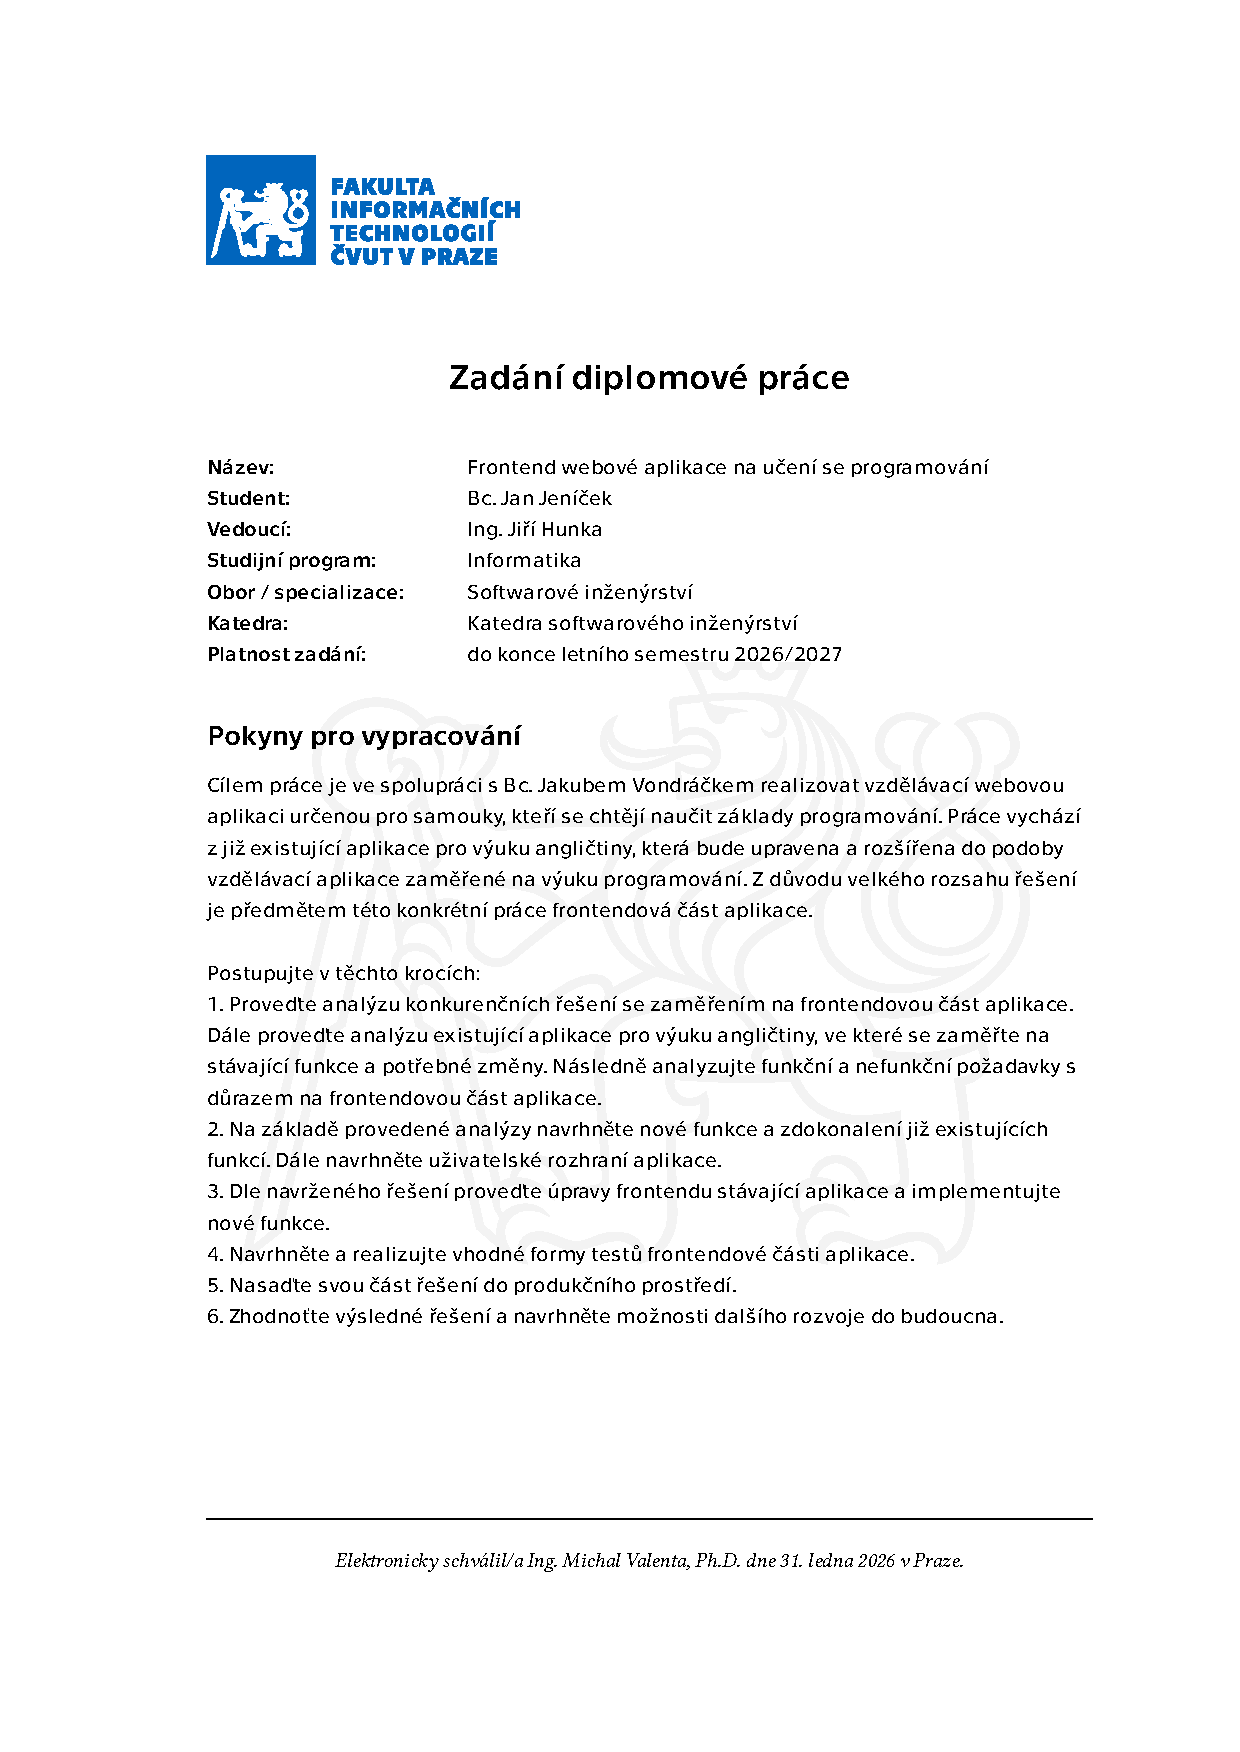
\includepdf[pages={1-}]{assignment-include.pdf} % replace this file with your thesis assignment generated from ProjectsFIT

\imprintpage % do not remove this command
\stopTOCentries
%%%%%%%%%%%%%%%%%%%%%%
% list of other contents END
%%%%%%%%%%%%%%%%%%%%%%

%%%%%%%%%%%%%%%%%%%
% ACKNOWLEDGMENT
% FILL IN / MODIFY
% This is a place to thank people for helping you. It is common to thank your supervisor.
%%%%%%%%%%%%%%%%%%%
% Final
\begin{acknowledgmentpage}
    Tímto bych chtěl poděkovat vedoucímu diplomové práce Ing.\,Jiřímu Hunkovi, zejména za cennou zpětnou vazbu, kterou mi poskytoval nejen v průběhu zpracovávání této práce, ale i během mých studií. Dále bych chtěl poděkovat kolegovi Bc. Jakubu Vondráčkovi za jeho vynikající práci, díky níž se nám podařilo vytvořit a nasadit funkční vzdělávací aplikaci. Poděkování patří také všem mým přátelům za podporu a motivaci během studia. Na závěr bych rád poděkoval své přítelkyni a rodině za jejich trpělivost a neustálou podporu.
\end{acknowledgmentpage}
%%%%%%%%%%%%%%%%%%%
% ACKNOWLEDGMENT END
%%%%%%%%%%%%%%%%%%%


%%%%%%%%%%%%%%%%%%%
% DECLARATION
% FILL IN / MODIFY
%%%%%%%%%%%%%%%%%%%
% INSTRUCTIONS
% ENG: choose one of approved texts of the declaration. DO NOT CREATE YOUR OWN. Find the approved texts at https://courses.fit.cvut.cz/SFE/download/index.html#_documents (document Declaration for FT in English)
% CZE/SLO: Vyberte jedno z fakultou schvalenych prohlaseni. NEVKLADEJTE VLASTNI TEXT. Schvalena prohlaseni najdete zde: https://courses.fit.cvut.cz/SZZ/dokumenty/index.html#_dokumenty (prohlášení do ZP)
% Final (Text prohlášení 1 – univerzální) + prohlášení o použití nástrojů umělé inteligence
\begin{declarationpage}
Prohlašuji, že jsem předloženou práci vypracoval samostatně a že jsem uvedl veškeré použité informační zdroje v souladu s Metodickým pokynem o dodržování etických principů při přípravě vysokoškolských závěrečných prací.

Beru na vědomí, že se na moji práci vztahují práva a povinnosti vyplývající ze zákona č. 121/2000 Sb., autorského zákona, ve znění pozdějších předpisů, zejména skutečnost, že České vysoké učení technické v Praze má právo na uzavření licenční smlouvy o užití této práce jako školního díla podle § 60 odst. 1 citovaného zákona.

Prohlašuji, že jsem v průběhu příprav a psaní závěrečné práce použil nástroje umělé inteligence. Vygenerovaný obsah jsem ověřil. Stvrzuji, že jsem si vědom, že za obsah závěrečné práce plně zodpovídám.
\end{declarationpage}
%%%%%%%%%%%%%%%%%%%
% DECLARATION END
%%%%%%%%%%%%%%%%%%%

% Use one of the two following commands. The first prints abstracts+keywords on two pages, the second puts them on one page (if possible). \printonepageabstract can also accept optional argument that specifies a vertical space before both abstracts (the default is 18 mm).
\printtwopageabstract
%\printonepageabstract 

%%%%%%%%%%%%%%%%%%%
% SUMMARY
% FILL IN / MODIFY
% OR REMOVE ENTIRELY (upon agreement with your supervisor)
% (appropriate to remove in most theses)
%%%%%%%%%%%%%%%%%%%
% \begin{summarypage}
% \section*{Summary section}
% 
% \lipsum[1][1-8]
% 
% \section*{Summary section}
% 
% \lipsum[2][1-6]
% 
% \section*{Summary section}
% 
% \lipsum[3]
% 
% \section*{Summary section}
% 
% \lipsum[2]
% 
% \section*{Summary section}
% 
% \lipsum[1][1-8] Lorem lorem lorem.
% \end{summarypage}
%%%%%%%%%%%%%%%%%%%
% SUMMARY END
%%%%%%%%%%%%%%%%%%%

\tableofcontents % do not remove this command
%%%%%%%%%%%%%%%%%%%%%%
% list of other contents: figures, tables, code listings, algorithms, etc.
% add/remove commands accordingly
%%%%%%%%%%%%%%%%%%%%%%
\listoffigures % list of figures
\begingroup
\let\clearpage\relax
\listoftables % list of tables. Remove if you do not have any.
\thectufitlistingscommand{} % list of code listings. Remove if you do not have any.
\thectufitlistofalgorithmscommand{} % list of algorithm pseudocodes defined using the algorithm package.
\endgroup

%%%%%%%%%%%%%%%%%%%
% ABBREVIATIONS
% FILL IN / MODIFY
% OR REMOVE ENTIRELY
% List the abbreviations in lexicography order.
%%%%%%%%%%%%%%%%%%%
\chapter{\thectufitabbreviationlabel}

% Final
\begin{tabular}{rl}
    WCAG 2.2 & Web Content Accessibility Guidelines 2.2 \\
    TDD & Test-Driven Development \\
    BDD & Behavior-Driven Development \\
    REST & Representational State Transfer \\
	API   & Application Programming Interface                 \\
	UI   & User Interface                 \\
	XP   & Experience Points                 \\
    AI   & Artificial Intelligence                 \\
    IDE  & Integrated Development Environment                 \\
    CLI  & Command Line Interface                 \\
    PWA  & Progressive Web Application                 \\
    CI/CD & Continuous Integration/Continuous Delivery                 \\
\end{tabular}
%%%%%%%%%%%%%%%%%%%
% ABBREVIATIONS END
%%%%%%%%%%%%%%%%%%%
\resumeTOCentries
\mainmatter\mainmatterinit % do not remove these two commands
%%%%%%%%%%%%%%%%%%%
% THE THESIS
% MODIFY ANYTHING BELOW THIS LINE
%%%%%%%%%%%%%%%%%%%

% Chapter: Introduction
%---------------------------------------------------------------
\chapter*{Úvod}\addcontentsline{toc}{chapter}{Úvod}\markboth{Úvod}{Úvod}
%---------------------------------------------------------------
\setcounter{page}{1}

% Done - Introduction why this project is needed
V posledních letech dochází k výrazným změnám v oblasti vzdělávání, a to zejména díky rozvoji nových technologií a metod učení. Stále větší popularitu získává mikrolearning, tedy učení prostřednictvím krátkých a efektivních lekcí. Ten však zatím není ve většině oborů dostatečně rozšířen. S nástupem umělé inteligence, zejména velkých jazykových modelů, se také zásadně mění možnosti, jak efektivně a personalizovaně přistupovat k učení. Tradiční systémy, jako jsou například vzdělávací kurzy nebo aplikace využívající spaced repetition algoritmy, často nedokáží držet krok s tímto rychlým vývojem. V moderních aplikacích je navíc kladen čím dál tím větší důraz na uživatelskou zkušenost, která stále u mnoha vzdělávacích systémů není na dostatečně vysoké úrovni.

% Done - Main goal of the project
Na základě těchto skutečností jsme se rozhodli s kolegou Bc. Jakubem Vondráčkem vytvořit moderní vzdělávací systém ve formě webové aplikace, který bude reflektovat aktuální změny v oblasti vzdělávání. Hlavním cílem této aplikace je propojit efektivní metody učení, s kvalitní uživatelskou zkušeností a možnostmi, které poskytuje umělá inteligence. V rámci této práce bude aplikace zaměřena především na výuku programování a softwarového inženýrství. Bude ovšem navržena tak, aby byla snadno rozšiřitelná a využitelná v různých oblastech vzdělávání. Důraz bude kladen na zábavnost, efektivitu a personalizaci učení, které jsou klíčové pro dlouhodobou motivaci uživatelů.

% Write - Rozšíření existujícího systému
Systém bude rozšířením již existující aplikace na výuku jazyků, kterou jsme společně s kolegou Bc. Janem Hlaváčem vytvořili v rámci našich bakalářských prací. Díky tomu bude možné projekt stavět na již vybudovaných základech a zaměřit se tak na implementaci pokročilejších funkcionalit. % Přidat citaci na moji a Honzovu práci? Dozjistit, jestli se může v úvodu citovat - nejspíš ano

% Done - Division into two master theses
Projekt byl rozdělen do dvou diplomových prací. Tato práce bude zaměřena na podrobnější analýzu požadavků a následný vývoj frontendové části aplikace. Diplomová práce kolegy Bc. Jakuba Vondráčka se pak bude převážně zabývat vývojem backendové části této aplikace.

% Done - Subgoals
Z hlavního cíle vytvoření vzdělávací aplikace přirozeně vyplývají dílčí cíle, které reflektují jednotlivé fáze životního cyklu softwarového projektu. Prvním cílem je provést analýzu existující aplikace na výuku jazyků a sepsat požadavky, které budou sloužit jako podklad % Zde nevím, jestli podklad je vhodné slovo, ale asi ano
pro vytvoření nové aplikace. V rámci analýzy bude také provedena analýza konkurenčních řešení v oboru výuky softwarového inženýrství. Druhým cílem je sepsat specifikaci nových funkcionalit a navrhnout jejich uživatelské rozhraní. Součástí tohoto cíle je také provedení aktualizace vzhledu existujícího uživatelského rozhraní. Třetím cílem je provedení samotné implementace funkcionalit a popsání použitých postupů a nově zavedených technologií. Čtvrtým cílem je zvolit a provést vhodné formy testování nových funkcionalit. Posledním cílem je pak zhodnocení celého řešení a navrhnutí možných úprav do budoucna.

% Done - Disclaimer
Práce bude zaměřena výhradně na vývoj aplikace a nebude zahrnovat vytváření samotného obsahu, jako například tvorbu konkrétních kurzů, lekcí nebo cvičení.

% Done - How the project will benefit others
Výsledná aplikace bude sloužit studentům a samoukům, kteří chtějí rozvíjet své znalosti a systematicky se zdokonalovat napříč různými obory. Výstup této práce bude mít největší přínos pro uživatele, kteří se chtějí vzdělat v oblastech programování a softwarového inženýrství, zároveň díky její rozšiřitelnosti bude možné aplikaci využít i v mnoha dalších oborech.


% Chapter: Analysis
% Done
\chapter{Analýza}

% Final
V první fázi vývoje se zaměřím na analýzu. Nejprve provedu analýzu stávající aplikace na výuku angličtiny. V rámci této analýzy se zaměřím na existující funkce, kód, testy a stávající návrh uživatelského rozhraní.

% Final
Dále provedu analýzu konkurenčních aplikací, které se zaměřují na výuku programování a softwarového inženýrství. Tato analýza bude sloužit zejména jako podklad pro sepsání požadavků a pro návrh jednotlivých funkcí.

% Final
Na konci této kapitoly sepíšu funkční a nefunkční požadavky, ze kterých budu dále vycházet v kapitolách návrhu a implementace. 


% Subchapter: Existing solution analysis
% Done
\section{Analýza stávající aplikace}

% Review
Jako první krok analýzy jsem provedl analýzu existující aplikace. V této části textu nejprve popíšu strukturu celého projektu a následně se zaměřím na analýzu kódu, existujících funkcí, testů a návrhu uživatelského rozhraní frontendové části aplikace.

% Review
Existující aplikace je webová aplikace zaměřena na výuku anglického jazyka. Frontendová část aplikace je postavena na knihovnách React a Next.js. Dále aplikace využívá knihovnu komponentů uživatelského rozhraní Material UI a knihovnu Storybook pro dokumentaci jednotlivých komponentů aplikace. Celé uživatelské rozhraní včetně všech komponentů je navrženo v nástroji Figma. Aplikace je nasazena v testovacím prostředí, kde využívá mock API, a dále v produkčním prostředí, kde je napojena na reálné backendové API. \cite{Jenicek2024BachelorThesis}

% Review
Frontend aplikace komunikuje s backendovou částí přes REST API. Kromě samotného API existuje i mock tohoto api, který byl vytvořen pomocí nástroje Mockoon. Souběžně s mou diplomovou prací, která se týká frontendové části aplikace, se věnuje kolega Bc. Jakub Vondráček backendové části aplikace v rámci jeho diplomové práce. Proto s dále v rámci této analýzy a dalších částech textu budu věnovat zejména frontendové části aplikace. \cite{Jenicek2024BachelorThesis}

% Review
Kromě frontendové části a backendové části aplikace existují v rámci tohoto projektu také webové stránky a dále systém pro správu obsahu aplikace. Těmto částem projektu se v této práci věnovat nebudu, nicméně i tak je bude třeba zohlednit, například při tvorbě a návrhu komponentů uživatelského rozhraní.

% Review
\subsection{Analýza kódu}

% Review
Nejprve jsem provedl analýzu kódu aplikace, v rámci které jsem nalezl několik příležitostí ke zlepšení celkové kvality kódu. Zaprvé, některé části kódu, zejména komponenty týkající se učení a opakování látky, nejsou dobře rozšiřitelné. Komponenty nemají flexibilní strukturu a může tak být obtížné přidávat nové typy cvičení. Dále se v kódu nacházejí části, které jsou přímo spjaty s konkrétní doménou výuky jazyků, přestože by dané části kódu mohly být navrženy obecněji tak, aby byla implementace nezávislá na vyučované doméně. Proto by bylo vhodné tyto části změnit tak, aby bylo možné kód využívat nezávisle na vyučované doméně.

% Review
Všechny komponenty jsou v současné aplikaci seskupeny do jedné složky \texttt{components}, v rámci které jsou dále rozděleny do podsložek pro základní komponenty, složitější komponenty a komponenty týkající se rozložení stránek. Tato základní organizace komponentů může být vhodná pro malé projekty, nicméně s narůstajícím počtem komponentů a stránek může být značně nepřehledná a špatně udržitelná. Proto by bylo vhodné přeorganizovat komponenty například tak, aby byly stránky a komponenty seskupeny podle daných funkcí. Do globálních složek, jako například do složky \texttt{components}, by tak bylo možné vkládat pouze komponenty, které jsou sdíleny napříč jednotlivými funkcemi. Díky této struktuře by tak mohlo být snazší se v kódu orientovat a přidávat nové funkce a komponenty.

% Review
Základní komponenty aplikace by také bylo vhodné přesunout do samostatné knihovny, aby bylo možné tyto komponenty využívat ve všech částech projektu, jako například na webových stránkách, a zajistit tak konzistenci vzhledu napříč celým projektem.

% Review
Další příležitostí pro zlepšení kvality kódu jsou samotné třídy, se kterými frontend pracuje. Třídy v kódu jsou definovány ručně tak, aby reflektovaly OpenAPI specifikaci backendového API. Zásadní nevýhodou tohoto přístupu je časová náročnost definice a udržování jednotlivých tříd. Tento přístup dále může snadno vést k nekonzistencím mezi definovanými třídami a reálným API, což může vést k následným chybám v aplikaci. Z tohoto důvodu navrhuji zavést do kódu automaticky generované třídy na základě OpenAPI specifikace backendového API. Díky tomu pak budou třídy snadno udržitelné a bude zajištěna přesná konzistence mezi specifikací API a frontendovou částí aplikace.

% Review
V kódu je také používána řada knihoven a nástrojů, které nebyly za poslední 2 roky vůbec aktualizovány, přestože většina z nich vydala nové verze. Jejich aktualizace by tak mohla přinést řadu výhod, jako například vyšší stabilitu a bezpečnost aplikace nebo vyšší efektivitu vývoje. 

% Review
Za posledních několik let došlo k významnému nárůstu používání nástrojů umělé inteligence pro asistenci při tvorbě kódu, dokumentací a testů. Současný frontend aplikace ovšem vůbec není pro práci s těmito nástroji přizpůsoben. Proto by bylo vhodné zavést pravidla, konvence a konfigurace, které by umožnily vývojářům pracovat s těmito nástroji a zefektivnit tak celý proces vývoje aplikace.

% Review
Kromě samotného kódu jsem také nalezl možnost zlepšení nasazení aplikace. Současná aplikace je nasazena v testovacím prostředí, kde využívá mock API, a v produkčním prostředí, kde využívá produkční backendové API. Neexistuje ovšem testovací prostředí, kde by aplikace mohla být testována se skutečným API. Z tohoto důvodu by bylo vhodné toto prostředí vytvořit, aby v něm mohla být aplikace manuálně testována s reálným API před nasazením do produkčního prostředí. 

% Review
\subsection{Analýza testů}

% Review
V rámci mé bakalářské práce, která se věnovala frontendu stávající aplikace, jsem provedl testy použitelnosti s uživateli. Většina problémů, které byly v rámci těchto testů objeveny, byla již opravena, nicméně stále existují některé problémy, které opraveny nebyly. Tyto problémy jsou popsány v mé bakalářské práci a bude třeba je zohlednit při sestavování požadavků a při návrhu této aplikace. \cite{Jenicek2024BachelorThesis}

% Review
Frontend aplikace v současné době neobsahuje žádné automatizované testy. Jelikož se aplikace bude zásadně měnit a rozšiřovat, bude vhodné zavést určitou formu automatizovaných testů. Zavedení automatizovaných testů je také v souladu s mým návrhem úprav do budoucna, který jsem popsal v rámci mé bakalářské práce. \cite{Jenicek2024BachelorThesis}

% Review
V aplikaci dále existují základní nástroje pro formátování a kontrolu kvality kódu ESLint a Prettier. Tyto nástroje by ovšem mohly využívat přísnější pravidla a konvence pro zamezení vzniku nejednoznačného kódu a chyb. Z tohoto důvodu navrhuji aktualizovat tyto nástroje a jejich konfigurace.

% Review
\subsubsection{Analýza návrhu uživatelského rozraní}

% Review
Návrh uživatelského rozhraní stávající aplikace jsem provedl v rámci mé bakalářské práce v nástroji Figma. Při analýze tohoto návrhu jsem nalezl několik příležitostí ke zlepšení.

% Review
Zaprvé, komponenty a stránky aplikace by bylo vhodné lépe zorganizovat. V současné aplikaci je struktura přehledná, nicméně s narůstajícím počtem stránek a komponentů se může stát značně nepřehlednou.

% Review
Značným problémem je také samotná struktura komponentů. V současném návrhu jsou komponenty tvořeny tak, že rozšiřují či upravují komponenty externí knihovny komponentů. Knihovna ovšem často obsahuje zbytečně komplexní strukturu komponentů a parametrů, které nejsou v rámci návrhu této aplikace nijak využívány. Všechny komponenty jsou tak zbytečně komplexní a práce s nimi je neefektivní. Z tohoto důvodu by bylo vhodné zvolit jiný přístup při tvorbě komponentů, například využití jiné knihovny, nebo vytvoření komponentů ručně. 

% Review
Nakonec by bylo vhodné vytvořit stránku s přehledem stylů, barev a typografie, které aplikace využívá. Díky tomu by pak bylo možné se styly snadněji pracovat a upravovat je.

% Review
\subsection{Analýza existujících funkcí}

% Review
Jelikož bude aplikace zásadně měnit svoje zaměření z domény výuky jazyků na doménu výuky programování, je třeba odebrat některé přebytečné funkce, které již nebudou relevantní pro novou doménu. Mezi tyto funkce patří například cvičení týkající se výuky jazyků, správa vlastních kolekcí slovíček nebo možnost vybírání preferovaných témat slovní zásoby.

% Review
Kromě odstranění přebytečných funkcí bude dále třeba upravit některé existující funkce. Příkladem toho je stránka kurzu, která v současné době zobrazuje lekce ve formě bodů s ikonou, které jsou umístěny na čáře připomínající cestu kurzem. Lekce jsou tak na mapě reprezentovány pouze ikonou a zkráceným názvem. Přestože může být toto vyobrazení lekcí pro uživatele vizuálně poutavé, může být pro uživatele obtížné na první pohled poznat, co je obsahem dané lekce. Vyhledávání konkrétních lekcí také může být pro uživatele značně obtížné. S měnící se doménou tak bude třeba změnit i strukturu kurzů a jejich sekcí a lekcí, aby mohli uživatelé kurzy snadněji procházet a vyhledávat konkrétní lekce.

\subsection{Závěr analýzy}

V rámci analýzy stávající aplikace jsem tak nalezl řadu podnětů ke zlepšení celkové kvality aplikace. Tyto podněty budu brát ve všech následujících fázích vývoje, při specifikaci požadavků, návrhu funkcí a následné implementaci.


% Subchapter: Competitor analysis
% Done
\section{Analýza existujících řešení}

% Review
V této sekci se budu věnovat analýze existujících aplikací, které vyučují softwarové inženýrství a programování. Cílem této analýzy je zjistit, jakým způsobem existující aplikace přistupují výuce programování, jakou mají uživatelskou zkušenost a uživatelská rozhraní, jakými způsoby motivují uživatele k učení, jaké funkce poskytují zdarma a jaké jsou placené, a jaké jsou silné a slabé stránky těchto aplikací. Na konci této sekce se dále zaměřím na to, jakými způsoby se může aplikace, kterou budu v rámci této práce vytvářet, odlišit od existujících aplikací.

% Review
Pro analýzu jsem se rozhodl vybrat aplikace, které se podobají vizi tohoto projektu a budou tak přímou konkurencí vznikající aplikace. Vybíral jsem tedy mezi nejpoužívanějšími aplikacemi určenými pro samouky, které vyučují softwarové inženýrství a programování pomocí krátkých a interaktivních lekcí. Do analýzy jsem tak zahrnul aplikace Codecademy, Sololearn, Mimo a Scrimba.

% Review
Poznatky z této analýzy využiji při sepisování požadavků této aplikace, návrhu nových funkcí a nového vzhledu uživatelského rozhraní.


\subsection{Mimo}

% Final
První analyzovanou aplikací je aplikace Mimo\footnote{Dostupné na: \href{https://mimo.org/}{https://mimo.org/}}, která se nejvíce blíží vizi tohoto projektu a bude tak přímou konkurencí vznikající aplikace. Mimo se zaměřuje zejména na výuku moderních programovacích jazyků a frameworků. V době psaní této práce Mimo nabízí 9 kurzů, 4 tzv. kariérní cesty a má napříč platformami přes 40 milionů registrovaných uživatelů \cite{Mimo}. Mimo je k dispozici jako webová aplikace a dále také jako mobilní aplikace na platformách Android a iOS. Pro analýzu použiji primárně aplikaci na platformě Android.

% Final
\subsubsection{Vzhled a uživatelská zkušenost}

% Odstavec: Obecný dojem (komplexita/přehlednost UI, paleta barev, typografie)
% Final
Mimo se od dalších konkurentů liší zejména svým vzhledem uživatelského rozhraní a stylem výuky. Uživatelské rozhraní je velice minimalistické a přehledné. Místy může aplikace působit až příliš jednoduchým dojmem. Aplikace využívá fialovou monochromatickou paletu barev a celé rozhraní využívá spíše tmavší barvy. V rámci typografie Mimo využívá pro některé nadpisy neproporcionální písmo. To lze pozorovat zejména v mobilní aplikaci a na webových stránkách. Pro textové prvky pak využívá bezpatkové písmo Aeonik.

% Odstavec: Rozložení prvků na obrazovce (lekce v kurzu, učení)
% Final
Rozložení prvků na obrazovce je přehledné. Na hlavní stránce kurzu jsou umístěny jednotlivé lekce, které jsou vyobrazeny ve formě tlačítek na čáře připomínající cestu kurzem. Až po kliknutí na danou lekci se zobrazí její název a možnost spuštění dané lekce. Toto vyobrazení lekcí může na uživatele působit vizuálně poutavým dojmem, nicméně může být obtížné se pomocí něj orientovat v kurzu, protože o lekcích nejsou na první pohled zobrazeny žádné podrobnější informace.

% Odstavec: Navigace v aplikaci
% Final
Pro navigaci v mobilní aplikaci používá Mimo velice jednoduchou spodní navigační lištu s pouze pěti prvky. Díky tomu je navigace v aplikaci velice snadná a rychlá.

% Odstavec: Srovnání webového a mobilního prostředí
% Final
Webová verze aplikace Mimo je velice podobná mobilní verzi. Rozdíl je především v tom, že ve webové aplikaci jsou lekce vyobrazeny ve formě seznamu. Pro navigaci je použita horní navigační lišta a pro navigaci mezi kapitolami kurzu pak boční navigační lišta.

% Odstavec: Animace a efekty a mikro interakce
% Final
V aplikaci jsou použity animace a efekty velice zřídka. Některé prvky uživatelského rozhraní jsou animovány při jejich zobrazení. Při učení jsou také použity animace pro přechody mezi jednotlivými cvičeními.

% Final
\subsubsection{Způsoby učení}

% Struktura kurzu (lineární, tematické moduly, career paths, kapitoly atd.)
% Final
Jednotlivé kurzy jsou uspořádány do sekcí, které pak obsahují jednotlivé lekce. Lekce jsou uspořádány lineárně a uživatel se je musí učit v daném pořadí. Kromě kurzů Mimo nabízí tzv. kariérní cesty, které mají podobnou strukturu jako kurzy, nicméně většinou obsahují více témat.

% Jak se spustí učení a jak vypadá study session
% Final
Učení lze spustit kliknutím na danou lekci. Při učení se uživateli zobrazuje sekvence stránek na nichž se nachází buď vysvětlení dané látky nebo různá cvičení. Při vyplňování cvičení je typicky uživateli zobrazena otázka, na kterou musí odpovědět například vyplněním textového pole v kódu. Po vyplnění odpovědi se uživateli zobrazí, zda byla odpověď správná, a u cvičení se spustitelným kódem se uživateli zobrazí výstup takového kódu. V kurzu SQL je tak uživateli například po vyplnění odpovědi zobrazena tabulka s daty, která by byla výsledkem daného SQL dotazu. Po vyplnění odpovědi ve webové aplikaci má uživatel také možnost si nechat odpověď vysvětlit v chatovém okně pomocí chatbota.

% Druhy cvičení
% Final
V aplikaci se nachází několik typů cvičení, které lze rozdělit do následujících kategorií.

% Final
\paragraph{Otázka s více odpovědmi} Jedním z nejčastějších typů cvičení je otázka, která typicky obsahuje ukázku kódu, a výběr z několika odpovědí. Uživatel má za cíl zvolit jednu správnou odpověď.

% Final
\paragraph{Doplňování do kódu} Dalším častým typem cvičení je doplňování částí kódu. Aplikace uživateli v otázce zobrazí ukázku kódu, do které je třeba doplnit typicky několik slov nebo znaků. Doplňování je v některých případech usnadněno tím, že může uživatel slova a znaky vybírat z předdefinovaného seznamu. To může značně zrychlit procházení těchto cvičení, protože uživatel nemusí vše psát ručně.

% Final
Dále aplikace ve cvičeních využívá řadu komponentů pro vysvětlení a lepší pochopení dané látky. Příkladem toho jsou následující komponenty.

% Final
\paragraph{Tabulky} V některých kurzech, zejména v kurzech vyučující témata týkající se databází, jsou využívány tabulky s daty. Ty se zobrazují jednak jako součástí zadání cvičení a jednak jako výstup po vyplnění daného cvičení.

% Final
\paragraph{Výstup kódu v terminálu} Po vyplnění cvičení, které v zadání obsahuje spustitelný kód, může být uživateli zobrazen komponent připomínající terminál s výstupem takového kódu. Tyto komponenty jsou typicky zobrazovány například u kurzů, které vyučují konkrétní programovací jazyky.

% Final
\paragraph{Zobrazení webové stránky} Po vyplnění cvičení, které v zadání obsahuje kód a zaměřuje se na webové technologie, je typicky zobrazena ukázka webové stránky, která reprezentuje výstup daného kódu. Tento typ cvičení je využívaný zejména u výuky jazyků, jako například HTML, CSS nebo JavaScript. Dále je tento typ cvičení také využíván pro výuku frontend frameworků.

% Final
\subsubsection{Způsoby motivace uživatele}

% Jaké formy gamifikace aplikace používá
% Final
Mimo používá různé způsoby motivace uživatelů k učení. Jedním z těchto způsobů je gamifikace, kterou lze definovat jako použití prvků herního designu v mimoherních kontextech \cite{10.1145/2181037.2181040} (překlad autora). V aplikaci Mimo jsem identifikoval následující formy gamifikace.

% Final
\paragraph{Virtuální měna} V aplikaci je možné za plnění cvičení získávat virtuální měnu, za kterou je následně možné si kupovat různé položky v obchodě aplikace.

% Final
\paragraph{Streak} Aplikace zaznamenává, kolik dní v řadě uživatel splnil alespoň jednu lekci. Tato řada je nazývána streak. Pokud uživatel daný den nesplnil žádnou lekci, je mu jeho streak resetován. V obchodě aplikace si může uživatel zakoupit několik položek, které mu pomohou zachovat streak i přes to, že se daný den zapomněl učit. Uživatel si tak může preventivně zakoupit položku, která mu zajistí, že se streak nezruší, pokud se zapomene některý den učit. Svůj streak může uživatel také zpětně napravit zakoupením příslušné položky.

% Final
\paragraph{Streak výzva} V obchodě aplikace může uživatel za virtuální měnu zakoupit tzv. streak výzvu. Pokud uživatel splní výzvu, která spočívá v učení se každý den po dobu 7 dní, dostane jako odměnu určité množství virtuální měny.

% Final
\paragraph{Srdíčka} Uživatel má k dispozici 5 srdíček, o která přichází, pokud neodpoví správně na danou otázku v průběhu cvičení. Srdíčka se obnovují po určitém čase a uživatel je také může zakoupit za virtuální měnu.

% Final
\paragraph{Body XP} Za plnění jednotlivých lekcí v aplikaci uživatel může získat tzv. body XP, které reprezentují pokrok uživatele v rámci aplikace. Tyto body jsou následně zobrazeny na jeho profilu a ovlivňují jeho pozici v lize učení.

% Final
\paragraph{Liga učení} Uživatelé jsou každý týden rozřazeni do ligy, neboli skupiny uživatelů, na základě toho, kolik bodů XP získali v předchozím týdnu. Na profilu uživatele se pak zobrazuje, ve které lize se nachází.

% Final
\paragraph{Systém přátel} Mimo umožňuje uživatelům si přidávat ostatní uživatele do přátel a sledovat tak jejich pokrok v aplikaci.

% Final
\paragraph{Ikona aplikace} Mimo umožňuje uživateli si za virtuální měnu zakoupit a změnit ikonu aplikace.

% Final
\subsubsection{Placená verze}

% Free tier
% Final
Mimo nabízí uživatelům zdarma pouze prvních několik lekcí každého kurzu. Při učení se uživatelům zobrazují reklamy a učení je omezeno funkcí srdíček.

% Premium tier
% Final
Uživatelé, kteří si zaplatí premium účet, se mohou všechny kurzy a kariérní cesty učit bez omezení. Při učení se jim nezobrazují reklamy a nejsou omezeni funkcí srdíček. Uživatelé s premium účtem si navíc mohou po dokončení kurzu vygenerovat a stáhnout certifikát o dokončení daného kurzu. 

% Free tier
% Final
Aplikace nabízí sedmidenní zkušební verzi premium účtu zdarma na webových stránkách Mimo. Zkušební verzi lze také získat pozváním přátel do aplikace.

% Final
\subsubsection{Silné a slabé stránky}

% Silné stránky
% Final
Silnou stránkou aplikace Mimo je její jednoduchost používání a krátké lekce. Uživatel se tak může snadno učit v průběhu dne čistě s využitím mobilu, což může být praktické zejména pro uživatele, kteří mají omezený čas na učení.

% Final
Další silnou stránkou je použitá gamifikace, která může vést ke zvýšené motivaci uživatelů používat aplikaci pravidelně.

% Slabé stránky
% Final
Možnou nevýhodou minimalistického vzhledu aplikace může být pocit, který uživatelské rozhraní svým minimalismem vyvolává. Aplikace může místy působit až příliš jednoduše a vyvolat tak dojem, že je příliš jednoduchá na to, aby vyučovala komplexní a pokročilá témata, kterými jsou například programování a softwarové inženýrství. To by mohlo některé uživatele odradit, zejména ty, kteří potřebují daná témata znát na profesionální úrovni.

% Final
Další potenciální nevýhodou je samotná navigace v kurzu. Lekce kurzu jsou vyobrazeny vizuálně poutavým způsobem, nicméně najít konkrétní lekci kurzu může být pro uživatele velice obtížné, zejména v mobilní verzi aplikace.

% Final
\subsubsection{Další poznatky}

% Zajímavé funkce
% Final
Mimo kromě základních funkcí poskytuje také tzv. pískoviště, kde může uživatel vytvářet a spouštět svůj kód a vidět jeho výstup. V rámci této funkce jsou k dispozici pouze jazyky HTML, CSS a JavaScript a dále framework React.

% Final
Aplikace také poskytuje funkci, v rámci které může uživatel vytvořit vlastní webovou aplikaci přímo uvnitř Mimo. V rámci této funkce uživatel zadá umělé inteligenci, co chce vytvořit. Mimo pak uživateli nastaví virtuální prostředí se systémem souborů, kde umělá inteligence celý projekt připraví. Uživatel pak může tento projekt upravovat a spouštět přímo v Mimo. Uživatel si může v rámci této funkce zobrazit danou webovou stránku, soubory projektu a také jednoduché zobrazení tabulek v databázi. Celý projekt pak uživatel může publikovat na veřejně dostupné webové adrese. Tato funkce je pro uživatele bez premium účtu značně omezená.

% (Zajímavé detaily nebo cokoliv co mě napadne)

% Final
\subsection{Codecademy}

% Final
Druhou analyzovanou aplikací je aplikace Codecademy\footnote{Dostupné na: \href{https://www.codecademy.com/}{https://www.codecademy.com/}}. Codecademy je jednou z nejpopulárnějších platforem na výuku programování a softwarového inženýrství. Nabízí přes 800 kurzů \cite{CodecademyCourses} a má napříč platformami přes 50 milionů uživatelů \cite{CodecademyPartnerships}. Codecademy je k dispozici jako webová aplikace a dále také jako aplikace Codecademy Go, která je k dispozici na platformách Android a iOS.

% Final
Mobilní aplikace Codecademy Go obsahuje pouze jednoduché funkce pro opakování a procvičování látky. Hlavní náplň kurzů se však nachází ve webové aplikaci Codecademy. Proto se v této analýze primárně zaměřím na webovou aplikaci, nicméně zahrnu do ní i poznatky ze zmíněné mobilní aplikace.  

% Final
\subsubsection{Vzhled a uživatelská zkušenost}

% Odstavec: Obecný dojem (komplexita/přehlednost UI, paleta barev, typografie)
% Final
Codecademy na první pohled působí mnohem komplexnějším dojmem než předchozí analyzovaná aplikace Mimo. Design uživatelského rozhraní je spíše minimalistický, nicméně místy může stále působit příliš složitě. V aplikaci je jako barva pozadí využívána primárně světle růžová barva. Při učení je pak pro pozadí využívána bílá, černá nebo tmavě šedá barva. Pro tlačítka a další důležité prvky rozhraní pak aplikace využívá vysoce kontrastní barvy jako například modrou nebo žlutou. Co se typografie týče, Codecademy využívá napříč celou aplikací, s výjimkou bloků kódu, bezpatkové písmo Apercu.

% Odstavec: Rozložení prvků na obrazovce (lekce v kurzu, učení)
% Final
Rozložení prvků na obrazovce je poměrně přehledné a logické, nicméně některé prvky rozhraní mohou být pro uživatele zbytečně matoucí nebo složité. Kupříkladu hned na hlavní stránce kurzu se nachází výrazné tlačítko pro smazání pokroku celého kurzu. Přestože je tato funkce velice důležitá, nejspíše nebude tak často využívána a pozice a výraznost tohoto tlačítka může akorát mást uživatele a odpoutávat jeho pozornost.

% Final
Na hlavní stránce kurzu je obsah kurzu rozdělen do seznamu rozbalovacích modulů, v nichž se mohou nacházet různé lekce, kvízy nebo projekty. Struktura kurzu je tak uspořádána přehledně a je snadné se v ní orientovat.

% Odstavec: Navigace v aplikaci
% Final
Pro navigaci v aplikaci je využita horní navigační lišta, ve které se nachází rozbalovací menu s odkazy na všechny důležité části aplikace. Dále bývá na jednotlivých stránkách využívána levá boční navigační lišta, která slouží k navigaci mezi funkcemi, které jsou relevantní pro danou stránku.

% Odstavec: Srovnání webového a mobilního prostředí
% Final
Mobilní aplikace Codecademy Go je, co se funkcí týče, výrazně jednodušší. Umožňuje základní funkce zapisování si kurzů a učení se jednotlivých témat. V rámci kurzu jsou k dispozici pouze výrazně zjednodušené lekce, které se liší od lekcí a aktivit ve webové aplikaci.

% Odstavec: Animace a efekty a mikro interakce
% Final
V aplikaci jsou animace a efekty použity velice zřídka nebo téměř vůbec. Celá stránka tak působí velice statickým dojmem. 

% Final
\subsubsection{Způsoby učení}

% Struktura kurzu (lineární, tematické moduly, career paths, kapitoly atd.)
% Final
Co se struktury kurzů týče, Codecademy nabízí hned několik druhů kurzů. Mezi ně patří kurzy, kariérní cesty a cesty schopností. Všechny tyto druhy kurzů mají stejnou strukturu a liší se zejména svojí obsáhlostí. Dále Codecademy nabízí řadu doplňujících materiálů, kterými jsou různé nástroje pro učení, dokumentace, videa, články a další.

% Final
Jednotlivé kurzy jsou rozděleny do modulů. V nich se pak nachází různé lekce, kvízy, projekty, články nebo další aktivity.

% Jak se spustí učení a jak vypadá study session
% Final
Na hlavní stránce kurzu je uživateli zobrazeno tlačítko, které mu umožňuje spustit lekci nebo aktivitu, u které uživatel naposledy v rámci kurzu skončil. Jednotlivé lekce se pak typicky skládají ze cvičení, která zabírají přibližně 10 minut.

% Final
Cvičení se skládají z textového vysvětlení látky a dále jednotlivých úkolů. Uživatel má k dispozici textový editor, ve kterém může psát a editovat připravený kód. Dále má k dispozici okno, ve kterém je vidět výstup daného kódu.

% Final
Kromě zmíněných prvků cvičení si může uživatel také otevřít tzv. tahák se shrnutím daného tématu. Dále si může uživatel spustit přiložené YouTube video, ve kterém lektor prochází daným cvičením a vysvětluje jednotlivé kroky.

% Final
Učení je přehledné a uživatel má k dispozici dostatek materiálů pro procvičení a pochopení dané látky. Potenciální nevýhodou může být struktura samotných cvičení. Uživatel je nucen si před každým cvičením přečíst několik stránek textu, což může být pro uživatele zdlouhavé a nezáživné.

% Final
V rámci učení má uživatel k dispozici AI asistenta, který mu v chatovém okně může vysvětlit danou látku nebo poradit s řešením daného úkolu.

% Druhy cvičení
% Final
V rámci lekcí jsou uživateli zobrazována především cvičení, v nichž uživatel doplňuje a přepisuje připravený kód přímo v editoru, nebo píše kód od začátku na základě zadání.

% Final
V rámci kvízů jsou uživateli zobrazovány různé otázky, typicky formou výběru z několika odpovědí nebo výběru, zda je daný výrok pravdivý nebo nepravdivý.

% Final
Jednou z dostupných aktivit jsou takzvané projekty, které svou strukturou připomínají delší cvičení v jednotlivých lekcích. Hlavním rozdílem je, že uživatel nemá možnost nahlédnout do správného řešení a jeho řešení není nijak kontrolováno. Uživatel tak musí daný úkol vyřešit sám bez pomoci. Jednotlivé úkoly pak sám může označit za splněné.  

% Final
\subsubsection{Způsoby motivace uživatele}

% Jaké formy gamifikace aplikace používá
% Final
Na rozdíl od aplikace Mimo nepoužívá Codecademy zdaleka tolik forem gamifikace. Aplikace ovšem motivuje uživatele několika následujícími způsoby.

% Final
\paragraph{Ukazatele pokroku} Uživatel má jak na domovské stránce, tak na stránce kurzu k dispozici ukazatele pokroku, které znázorňují, kolik procent daného kurzu uživatel dokončil. 

% Final
\paragraph{Ocenění} Za splnění určitých cílů v rámci učení uživatel může získat různá ocenění, která se následně zobrazují na jeho profilu ve formě odznaků.

% Final
\paragraph{Certifikáty} Codecademy nabízí dva typy certifikátů. První typ certifikátu uživatel může získat po dokončení určitého kurzu. Druhý typ certifikátu je tzn. profesní certifikát. Ten může uživatel získat, pokud splní všechny testy v rámci dané kariérní cesty.

% Final
\paragraph{Streak} Podobně jako v aplikaci Mimo zaznamenává Codecademy streak uživatele, neboli počet dní, po které se uživatel alespoň jednou denně učil bez přerušení.

% Final
\paragraph{Sledování pokroku dovedností} Unikátní funkcí Codecademy je sledování pokroku u dané dovednosti. Když se uživatel například učí jazyk JavaScript, zvyšuje se mu dovednost vývoje webových aplikací. Uživatel si pak může u každé dovednosti zobrazit jeho úroveň, jak dobře danou látku ovládá a co by se měl například ještě naučit.

% Final
Celkově tak Codecademy obsahuje několik způsobů motivace uživatelů, nicméně zdá se, že má v aplikaci gamifikace spíše vedlejší roli.

% Final
\subsubsection{Placená verze}

% Final
Codecademy, na rozdíl od ostatních aplikací, neobsahuje žádné reklamy. Místo toho nabízí uživatelům několik různých modelů předplatného. Předplatné se dá rozdělit do kategorie pro samouky, studenty a firmy.

% Individual tier
% Final
V rámci kategorie předplatného pro samouky Codecademy nabízí uživatelům některé základní kurzy zdarma. V rámci předplatného Plus se pak mohou uživatelé učit neomezené množství kurzů a dostanou přístup k cestám schopností. Dále mohou neomezeně využívat AI asistenta při učení. Poslední předplatné Pro umožňuje uživatelům se učit pomocí kariérní cesty, získávat profesní certifikáty. Uživatelé s tímto předplatným mohou využívat další funkce aplikace, jako například simulátor pracovních pohovorů, programátorské výzvy a další.

% Premium tier
% Final
Codecademy dále nabízí předplatné pro studenty. Toto předplatné je takřka stejné jako Pro předplatné pro samouky. Hlavním rozdílem je snížená cena, pokud uživatel doloží jeho status studenta.  

% Free tier
% Final
Poslední kategorií předplatného je předplatné pro firmy. Toto předplatné má dvě varianty Teams a Enterprise. Teams nabízí podobné funkce jako Pro předplatné pro samouky s rozdílem, že firma dostane navíc možnost spravovat jednotlivé účty uživatelů, přiřazovat je do skupin a získávat přehledy o učení uživatelů. Enterprise navíc nabízí možnost integrací dalších aplikací a hodiny vedené online instruktorem.

% Final
\subsubsection{Silné a slabé stránky}

% Silné stránky
% Final
Jednou ze silných stránek Codecademy je velké množství výukových materiálů, které stránka nabízí. Uživatelé mají přístup ke kvízům, lekcím, videím, projektům, shrnutím látky a dalším nástrojům, které jim umožní se naučit danou látku.

% Final
Další silnou stránkou Codecademy je minimalistické uživatelské rozhraní. Přestože se některé části uživatelského rozhraní mohou zdát zbytečně složité, aplikace je celkově velice přehledná a snadná na používání, obzvláště pokud se vezme v úvahu množství materiálů, kurzů a funkcí, které aplikace nabízí.

% Slabé stránky
% Final
Jednou z potenciálních nevýhod Codecademy je právě samotné zobrazování vzdělávacích materiálů při učení. Na stránce cvičení má uživatel například přístup k zadání úkolu, vysvětlení látky ve formě textu, dále k videu vysvětlující látku, AI asistentovi, shrnutí látky, komunitní sekci a dalším podpůrným materiálům. Když uživatel prochází jednotlivými cvičeními, může se pak cítit přehlcen tím, že mu jsou všechny informace zobrazovány na jedné stránce.

% Final
Další potenciální nevýhodou Codecademy je nedostatek motivace uživatelů. Aplikace sice obsahuje několik forem gamifikace a motivace uživatele, nicméně zdá se, že tyto způsoby motivace mají v aplikaci spíše vedlejší roli.

% Final
Poslední nevýhodou této aplikace může být to, že je uživatel sám zodpovědný za opakování si dané látky. Pokud například uživatel dokončí kurz, aplikace předpokládá že danou látku uživatel zná a nepomáhá mu si danou látku opakovat. Uživatel tak může například po několika měsících látku zapomenout a pokud by ji následně potřeboval umět, musel by projít kurzem znovu.

% Final
\subsubsection{Další poznatky}

% Final
Kromě výše zmíněných výhod a nevýhod jsem v rámci analýzy narazil na několik funkcí, které stojí za zmínku.

% Zajímavé funkce
% Final
\paragraph{Formátování kódu v editoru} V rámci cvičení má uživatel k dispozici tlačítko, kterým může automaticky zformátovat napsaný kód v editoru. To může být velice užitečné a přispívat ke kvalitní uživatelské zkušenosti, protože uživatel nemusí kód formátovat manuálně.

% Final
\paragraph{Studijní plán} Codecademy umožňuje uživateli si vygenerovat studijní plán. V rámci plánu si může nastavit, jak dlouho a kolik dní v týdnu se chce učit. Aplikace mu pak každý den doporučí konkrétní lekce a aktivity, které má daný den projít. Limitací této funkce je, že si uživatel může sestavit plán pouze pro daný kurz a nemá možnost si vygenerovat plán, který by obsahoval více kurzů zároveň. Přesto může být tato funkce pro uživatele velice užitečná a může značně zjednodušit každodenní učení a mít tak pozitivní vliv na uživatelskou zkušenost.

% Final
\subsection{Sololearn}

% Final
Sololearn\footnote{Dostupné na: \href{https://www.sololearn.com/}{https://www.sololearn.com/}} je jednou z nejpopulárnějších aplikací na učení se softwarového inženýrství a programování. Nabízí přes 40 kurzů na různá témata napříč softwarovým inženýrstvím a má napříč platformami přes 58 milionů registrovaných uživatelů \cite{Sololearn}.

% Final
Sololearn je k dispozici jako webová aplikace a dále také jako mobilní aplikace na platformách Android a iOS. Pro analýzu použiji mobilní verzi aplikace pro platformu Android.

% Final
\subsubsection{Vzhled a uživatelská zkušenost}

% Odstavec: Obecný dojem (komplexita/přehlednost UI, paleta barev, typografie)

% Final
Design aplikace může na první pohled působit starším a lehce zvláštním dojmem, zejména kvůli nekonzistentnímu použití komponentů knihovny Material UI a bez dodržování doporučených standardů designu Material Design 2 \cite{MaterialDesignDensity}, podle kterých se tato knihovna řídí \cite{MaterialUI}. Uživatelské rozhraní tak místy působí příliš nepřehledně. Co se palety barev týče, používá Sololearn světle modrou jako primární barvu a světle zelenou jako sekundární barvu. Pro pozadí a plochy pak používá bílou a modrošedou barvu. V rámci typografie je napříč celou aplikací použito písmo Fira Sans, jen pro bloky kódu je použito neproporcionální písmo Fira Mono.

% Odstavec: Rozložení prvků na obrazovce (lekce v kurzu, učení)
% Final
Rozložení prvků na obrazovce je poměrně přehledné a logické. Místy může působit nepřehledně kvůli malému prostoru mezi jednotlivými prvky, malé velikosti textu a většímu nahuštění prvků uživatelského rozhraní na jednotlivých stránkách.

% Final
Na hlavní stránce kurzu jsou lekce seskupeny do sekcí, které může uživatel kliknutím rozbalit. Díky tomu si může uživatel jednoduše získat přehled o celém kurzu a rozbalit části, které ho zajímají.

% Odstavec: Navigace v aplikaci

% Final
Pro navigaci je v aplikaci použita dolní navigační lišta s pěti prvky a také boční navigační lišta s ostatními funkcemi. 

% Odstavec: Srovnání webového a mobilního prostředí

% Final
Webová verze aplikace Sololearn obsahuje méně funkcí než verze mobilní. V mobilní aplikaci je kromě základních funkcí také možné plnit programátorské výzvy, soutěžit ve výzvách proti ostatním uživatelům, číst články a procházet lekce vytvořené komunitou.  

% Odstavec: Animace a efekty a micro interakce
% Final
Sololearn využívá animace a efekty velice zřídka. Základní animace jsou použity zejména pro zobrazování prvků na obrazovce. Nejvíce animací je využito v animovaných obrázcích, které jsou zobrazovány po dokončení lekce nebo v úvodním registračním formuláři.

% Final
\subsubsection{Způsoby učení}

% Struktura kurzu (lineární, tematické moduly, career paths, kapitoly atd.)
% Final
Kurzy jsou v aplikaci rozděleny do sekcí, ve kterých se nacházejí jednotlivé lekce a kvízy. Díky této jednoduché struktuře je velice snadné se v kurzech orientovat. Potenciální nevýhodou této jednoduché struktury může být to, že se pak v delších kurzech nachází příliš mnoho sekcí, což může být pro uživatele nepřehledné.

% Jak se spustí učení a jak vypadá study session
% Final
Pro spuštění učení uživatel přejde na stránku kurzu, kde se u nadcházející lekce nachází tlačítko pro spuštění učení. Samotné učení se velice podobá učení v aplikaci Mimo. Skládá se ze série stránek vysvětlujících danou látku a krátkých cvičení, při kterých si uživatel látku procvičí. Po zodpovězení otázky si uživatel může také zobrazit diskuzi a komentáře ostatních uživatelů k danému cvičení. Na rozdíl od aplikace Mimo se po dokončení cvičení nezobrazuje automaticky výstup daného kódu. Uživateli je jen zobrazeno, zda odpověděl správně nebo špatně a může si nechat jeho odpověď vysvětlit pomocí umělé inteligence. Na konci každé lekce je uživateli zobrazeno shrnutí s klíčovými informacemi, které by si měl z lekce odnést.

% Druhy cvičení
% Final
Sololearn nabízí v rámci učení různé druhy cvičení. Nejčastěji se jedná o doplňování slov z nabídky do kódu nebo textu. Dalším častým typem cvičení je výběr správné odpovědi z nabídky. Sololearn také nabízí cvičení, v rámci kterého může uživatel psát celý kód a zobrazovat si jeho výstupy. Celou strukturou učení se tak velice podobá analyzované aplikaci Mimo.

% Final
\subsubsection{Způsoby motivace uživatele}

% Jaké formy gamifikace aplikace používá
% Final
Sololearn pro motivaci uživatelů využívá několik forem gamifikace. Podobně jako aplikace Mimo využívá streak uživatele, srdíčka při učení, body XP, ligu učení a virtuální měnu.

% Final
Kromě těchto forem gamifikace jsou uživateli také zobrazovány na různých místech v aplikaci indikátory pokroku, které zobrazují, jakou část jednotlivých kurzů uživatel dokončil.

% Final
\subsubsection{Placená verze}

% Final
Aplikace nabízí uživatelům dva typy předplatných Sololearn Pro a Sololearn Max.

% Free tier
% Final
Uživatelé bez předplatného mohou procházet standardní lekce ve všech kurzech. Jediným omezením je počet srdíček, které uživatelé mají k dispozici. Uživatelům jsou také po dokončení lekcí zobrazovány reklamy.

% Pro tier
% Final
Uživatelé s předplatným Pro mají přístup k speciálním lekcím v kurzech, ve kterých si mohou procvičit programátorské úlohy zaměřené na reálné problémy z praxe. Dále mají k dispozici neomezený počet srdíček, nejsou jim zobrazovány reklamy a mají přístup k dodatečným materiálům a kvízům.

% Max tier
% Final
Předplatné Max kromě zmíněných výhod nabízí uživateli také možnost využít umělou inteligenci, aby mu pomohla při učení. Díky ní si uživatel může nechat vysvětlit daný kus kódu, proč byla jeho odpověď špatná, a jak by ji měl opravit.

% Final
\subsubsection{Silné a slabé stránky}

% Silné stránky
% Final
Silnou stránkou této aplikace je přehlednost a jednoduchá struktura jednotlivých kurzů. Pro obsáhlejší kurzy může být tato struktura nepřehledná, nicméně pro malé a středně velké kurzy, které se v aplikaci vyskytují, může být tato struktura vhodná.

% Final
Další silnou stránkou je samotné učení. Stránky s vysvětlením látky i cvičení se snadno používají. Látka tak může být pro uživatele mnohem stravitelnější, než například ve cvičeních konkurenční aplikace Codecademy.

% Final
Poslední silnou stránkou Sololearn je motivace uživatele. Aplikace využívá řadu mechanismů pro motivaci uživatele, které mohou přimět uživatele pravidelně aplikaci používat. 

% Slabé stránky
% Final
Jednou ze slabých stránek Sololearn je design některých stránek. Kvůli nedodržení některých standardů designu mohou stránky působit na uživatele příliš nepřehledně a zastaralým dojmem.

% Final
Druhou slabou stránkou aplikace je délka úvodního dotazníku při registraci uživatele. Dotazník obsahuje přes 10 stránek, což může být pro některé uživatele potenciálně odrazující. Založení účtu tak trvá výrazně déle, než u ostatních aplikací. 

% Final
\subsubsection{Další poznatky}

% Zajímavé funkce

% Final
Při učení aplikace na mobilu umožňuje uživateli přejet prstem po obrazovce doleva nebo doprava a tím přecházet mezi již dokončenými cvičeními v rámci dané lekce. Díky tomu se může uživatel velice jednoduše vrátit k předchozím cvičením a stránkám, které vysvětlují danou látku.

% Final
Další funkcí, která stojí za pozornost, je dostupné a snadné přepínání mezi zapsanými kurzy. Na rozdíl od ostatních aplikací, kde uživatel musí pro přepnutí mezi kurzy přejít na samostatnou stránku, může v Sololearn uživatel jednoduše přepnout kurz kliknutím na název kurzu v horní navigační liště, čímž se rozbalí seznam zapsaných kurzů, ze kterých si může uživatel jeden kurz vybrat a přesunout se tak na jeho hlavní stránku. Díky tomu může uživatel snadno přecházet mezi zapsanými kurzy, aniž by se musel přesouvat na samostatnou stránku se seznamem kurzů. To může být velice užitečné zejména pro uživatele, kteří se chtějí učit více kurzů zároveň a potřebují tak mezi kurzy často přepínat.

% Final
\subsubsection{Celkové hodnocení}

% Final
Souhrnné hodnocení aplikace Sololearn je uvedeno v tabulce \ref{table:competitor-rating-sololearn}.

% Final
\begin{table}[ht]
    \centering
    \begin{tabular}{@{} l c @{}}
        \toprule
        Oblast hodnocení & Hodnocení \\
        \midrule
        Uživatelská zkušenost & 5/10 \\
        Jednoduchost učení & 6/10 \\
        Podpora opakování & 4/10 \\
        Motivace uživatelů & 7/10 \\
        Interaktivita cvičení & 5/10 \\
        \bottomrule
    \end{tabular}
    \captionsetup{justification=centering}
    \caption{Hodnocení aplikace Sololearn}
    \label{table:competitor-rating-sololearn}
\end{table}

% Final
\subsection{Scrimba}

% Final
Poslední analyzovanou aplikací je webová aplikace Scrimba\footnote{Dostupné na: \href{https://scrimba.com/}{https://scrimba.com/}}. Tato aplikace se od ostatních odlišuje zejména svým inovativním způsobem výuky programování, který kombinuje prostředí připomínající skutečné IDE a interaktivní výuková videa. Lekce se tak odehrávají přímo v editoru kódu, ve kterém je uživateli vysvětlována látka a zadávány úkoly. Tento přístup výuky může přinést řadu výhod oproti tradičním metodám výuky a proto jsem se rozhodl tuto aplikaci do analýzy zahrnout.

% Final
Platforma Scrimba obsahuje přes 80 kurzů na různá témata napříč softwarovým inženýrstvím \cite{ScrimbaCourses}. V době psaní tohoto textu jsou kurzy zaměřeny zejména na webové technologie a umělou inteligenci.

% Final
Na rozdíl od ostatních analyzovaných aplikací Scrimba nemá v současné době mobilní verzi aplikace. Proto pro analýzu využiji dostupnou webovou aplikaci Scrimba. 

% Final
\subsubsection{Vzhled a uživatelská zkušenost}

% Odstavec: Obecný dojem (komplexita/přehlednost UI, paleta barev, typografie)

% Final
Na první pohled působí Scrimba jako přehledná a minimalistická aplikace. Ve srovnání s konkurenční aplikací Mimo používá aplikace menší velikost písma a zobrazuje na stránkách více textu. Aplikace tak může působit komplexnějším dojmem. Co se palety barev týče, používá Scrimba monochromatickou paletu modré barvy. Odstíny modré jsou použity pro pozadí, primární akce, ikony i textové prvky. Pro upozornění a některé štítky aplikace výjimečně využívá žlutou nebo zelenou barvu. Napříč aplikací je použito systémové písmo, tedy písmo, které je nastaveno v závislosti na operačním systému uživatele. Na systému Windows je tak použito například písmo Segoe, na zařízeních macOS pak písmo San Francisco a na zařízeních Android písmo Roboto \cite{SystemFontWebSafeFont}.

% Odstavec: Rozložení prvků na obrazovce (lekce v kurzu, učení)
% Final
Prvky jsou na obrazovce rozloženy velice přehledně a logicky. Ve srovnání s ostatními aplikacemi Scrimba používá méně prostoru mezi jednotlivými prvky uživatelského rozhraní. V důsledku toho může aplikace působit komplexnějším dojmem.

% Final
Na hlavní stránce kurzu jsou jednotlivé sekce, moduly a lekce vizuálně uspořádány do stromové struktury, kterou lze postupně rozbalovat. Díky tomu může uživatel jednoduše získat přehled o celém kurzu a rozbalit části, které ho zajímají. Obsah kurzu je tak uspořádán velice přehledně.

% Odstavec: Navigace v aplikaci

% Final
Na rozdíl od ostatních analyzovaných aplikací Scrimba nevyužívá pro navigaci horní navigační lištu, ani žádnou patičku stránky. Pro navigaci je využívána výhradně boční navigační lišta, která je umístěna na levé straně obrazovky.

% Odstavec: Animace a efekty a mikro interakce

% Final
Ve srovnání s ostatními aplikacemi Scrimba výrazně více využívá animace jednotlivých prvků uživatelského rozhraní a animované přechody mezi stránkami. Na většině stránek aplikace jsou při načtení zobrazeny animace některých prvků rozhraní. Další výraznou animaci lze zpozorovat při přejetí kurzorem nad tlačítko. Při animaci je tlačítko zvýrazněno čarou, která ho postupně obklopí po jeho obvodu.

% Final
Animace jsou tak napříč aplikací používány často, nicméně minimalisticky a v přiměřeném množství. Díky tomu Scrimba může působit výrazně interaktivnějším a vizuálně poutavějším dojmem, než její konkurenti.

% Final
\subsubsection{Způsoby učení}

% Struktura kurzu (lineární, tematické moduly, career paths, kapitoly atd.)

% Final
Scrimba nabízí, podobně jako ostatní analyzované aplikace, kurzy a kariérní cesty. Kariérní cesty jsou takřka stejné jako kurzy a liší se pouze v tom, že obsahují více témat. Lekce v kurzech jsou uspořádány chronologicky a seskupeny do kapitol a podkapitol.

% Jak se spustí učení a jak vypadá study session

% Final
Unikátní funkcí této aplikace je samotné učení. Při spuštění učení je uživateli v prohlížeči zobrazen editor připomínající skutečné IDE, ve kterém je možné prohlížet soubory a editovat kód. V editoru zároveň uživatel vidí okno s výstupem daného kódu. Dále je uživateli zobrazena prezentace doplňující výklad dané látky. Všechna tato okna může uživatel v průběhu výkladu schovávat, zobrazovat a procházet dle libosti.

% Final
Při učení uživatel poslouchá audio s vysvětlením dané látky. V průběhu toho je mu buď zobrazena prezentace nebo editor, ve kterém může sledovat, jak lektor přepisuje kód a jak pohybuje svým kurzorem myši. Při výkladu může uživatel procházet libovolné soubory a přepisovat jejich obsah. Dále si může kdykoliv zobrazit okno s prezentací nebo výstupem kódu. Audio s výkladem látky může uživatel kdykoliv přetáčet zpět a nebo dopředu. V průběhu lekce jsou uživateli zadávány úkoly, které musí v editoru splnit. Zadání je provedeno lektorem v audio nahrávce. Po zadání úkolu je audio pozastaveno, dokud uživatel nesplní daný úkol. 

% Druhy cvičení
% Final
Na rozdíl od ostatních analyzovaných aplikací Scrimba nepoužívá předdefinované typy cvičení. Veškerý výklad látky i cvičení se odehrávají přímo v editoru. Cvičení typicky spočívají v úpravě existujícího kódu nebo napsání nového kódu. Celkově je učení velice interaktivní a připomíná kombinaci videí s výkladem a skutečného IDE. Tato forma učení může být pro uživatele velice přínosná, zejména kvůli názornějšímu vysvětlení látky a interaktivnímu způsobu učení.

% Final
\subsubsection{Způsoby motivace uživatele}

% Jaké formy gamifikace aplikace používá
% Final
Na rozdíl od ostatních aplikací Scrimba neobsahuje téměř žádné formy gamifikace. Uživatelé nesbírají žádné body nebo ocenění, a nemohou spolu v aplikaci interagovat. Motivující pro uživatele ovšem může být, že aplikace jasně ukazuje, kolik procent kurzu uživatel dokončil a kolik cvičení uživatel splnil. Všechny splněné lekce jsou také označeny výraznou zelenou barvou a ikonou zaškrtnutí. Tato vizuální indikace pokroku může pro některé uživatele sloužit jako zdroj motivace.

% Final
\subsubsection{Placená verze}

% Final
Scrimba na rozdíl od ostatních aplikací neobsahuje žádné reklamy a nabízí pouze jeden model předplatného.

% Free tier
% Final
Uživatelé bez předplatného mají k dispozici většinu kurzů zdarma. Některé kurzy a kariérní cesty jsou ovšem k dispozici pouze uživatelům s aktivním předplatným. V nich mají uživatelé bez předplatného možnost si vyzkoušet několik prvních lekcí.

% Premium tier
% Final
Uživatelé s aktivním předplatným mají kromě základních kurzů přístup k pokročilejším kurzům a kariérním cestám. Na konci každého kurzu si navíc mohou vygenerovat a stáhnout certifikát o dokončení daného kurzu.

% Final
\subsubsection{Silné a slabé stránky}

% Silné stránky
% Final
Silnou stránkou této aplikace je její unikátní přístup k učení. Uživatelé se učí přímo v editoru připomínající IDE a veškerá látka je vysvětlena lektorem a doplněna o prezentaci s obrázky, GIFy a diagramy. Učení je tak zábavné, interaktivní a může být pro uživatele více srozumitelné, zejména u složitější látky.

% Final
Další silnou stránkou aplikace je minimalistický design a rozložení obsahu. Aplikace se velice snadno používá a je velice jednoduché najít, co uživatel potřebuje. Důvodem může být také to, že aplikace obsahuje pouze funkce, které jsou klíčové pro výuku programování a nezahlcuje uživatele dodatečnými materiály a nástroji.

% Slabé stránky
% Final
Mírnou nevýhodou inovativního způsobu učení je volnost uživatele při učení. Uživatel může v průběhu výkladu svým počínáním například omylem vypnout okno s prezentací nebo výstupem kódu. Proto se může velice jednoduše stát, že lektor v audio nahrávce mluví například o diagramu v prezentaci, který se uživateli na obrazovce nezobrazuje, protože uživatel dříve kliknul na editor, což zamezilo zobrazení okna s prezentací. Pro uživatele tak může být místy velice matoucí, kde se zrovna lektor nachází v průběhu výkladu a může být těžké výklad sledovat.

% Final
Další potenciální nevýhodou může být nedostatek motivace uživatele. Aplikace neobsahuje téměř žádné funkce, které by se zaměřovaly na dlouhodobou motivaci uživatelů. Proto může být pro uživatele obtížné se dlouhodobě přimět k používání této aplikace.

% Final
Poslední slabou stránkou aplikace Scrimba je místy nefunkční editor kódu. Protože do kódu může zároveň zapisovat virtuální lektor a uživatel, několikrát se při mým průchodem aplikací stalo, že byl například kurzor posunutý o několik znaků vedle, nebo že psaní do kódu nefungovalo a přepisovaly se jiné znaky, než by uživatel očekával. Tento problém může být pro uživatele velice odrazující při používání aplikace, protože se pak aplikace jeví jako nefunkční.

% Final
\subsubsection{Další poznatky}

% Zajímavé funkce
% Final
V rámci analýzy jsem došel k pozoruhodnému poznatku. Na rozdíl od ostatních aplikací Scrimba nemá dedikovanou domovskou stránku, která by například uživateli prezentovala výhody aplikace a jiné marketingové materiály. Místo toho je uživateli na hlavní stránce zobrazen seznam všech kurzů a krátké video popisující, jak se aplikace používá. Uživatelské rozhraní nepřihlášeného a přihlášeného uživatele se tak téměř neliší. Uživatelé mohou prohlížet všechny kurzy bez přihlášení a mohou spustit až dvě libovolné lekce, než po nich bude aplikace vyžadovat přihlášení. Díky tomu mohou uživatelé zjistit, zda jim vyhovuje formát výuky, než se do aplikace zaregistrují.

% Final
\subsubsection{Celkové hodnocení}

% Final
Souhrnné hodnocení aplikace Scrimba je uvedeno v tabulce \ref{table:competitor-rating-scrimba}.

% Final
\begin{table}[ht]
    \centering
    \begin{tabular}{@{} l c @{}}
        \toprule
        Oblast hodnocení & Hodnocení \\
        \midrule
        Uživatelská zkušenost & 8/10 \\
        Jednoduchost učení & 5/10 \\
        Podpora opakování & 3/10 \\
        Motivace uživatelů & 3/10 \\
        Interaktivita cvičení & 9/10 \\
        \bottomrule
    \end{tabular}
    \captionsetup{justification=centering}
    \caption{Hodnocení aplikace Scrimba}
    \label{table:competitor-rating-scrimba}
\end{table}

% Final
\subsection{Závěr analýzy}

% Final
V této části textu shrnu nejdůležitější výstupy provedené analýzy konkurenčních řešení. Tyto výstupy budou sloužit jako podklad pro sestavení požadavků tohoto projektu.

% Final
\subsubsection{Vzhled a uživatelská zkušenost}

% Final
Většina aplikací se snaží poskytnout uživateli přehledný a snadno použitelný způsob učení. Vzhled uživatelského rozhraní je u většiny aplikací minimalistický. Tomu odpovídá i struktura stránek a samotných kurzů, která bývá velice jednoduchá.

% Final
Aplikace často používají animace a další vizuální efekty, aby udělaly učení a používání aplikace vizuálně poutavější. To může potenciálně pomoci udržet pozornost uživatele při učení. Současná aplikace animace a efekty téměř nepoužívá a proto stojí za zvážní jejich použití.

% Final
\subsubsection{Způsob výuky}

% Final
Analyzované aplikace volí různé způsoby výuky. Aplikace Mimo a Sololearn učí uživatele pomocí krátkých cvičení, Codecademy pomocí delších úkolů a Scrimba pomocí vysoce interaktivních lekcí. Každý způsob výuky poskytuje určité výhody a nevýhody a bude třeba zvážit, který způsob je pro uživatele nejvhodnější.

% Final
V rámci učení jsou uživateli zobrazovány různé typy cvičení. Typicky se jedná o doplňování slov do kódu, psaní kódu do editoru a výběr správné odpovědi z nabídky.

% Final
Ve většině aplikací je uživateli látka vysvětlena pomocí krátkých textových popisů. Výjimkou je aplikace Scrimba, ve které je látka uživateli vysvětlena pomocí audio nahrávky v kombinaci s prezentací a interaktivním editorem. Použití audio nahrávek a interaktivních prvků může být pro uživatele potenciálně poutavější a srozumitelnější, než pouhé čtení textu. Podobnou formu výuky bude vhodné zvážit při návrhu struktury učení v této práci.

% Final
Většina aplikací také zobrazuje lekce kurzu ve formě seznamu. To se zásadně liší od současné aplikace, ve které jsou lekce vizuálně uspořádány do tvaru připomínající cestu kurzem. Přestože tato struktura může být vizuálně poutavější, a například aplikace Mimo ji také využívá, bude třeba zvážit, zdali by pro uživatele nebylo přehlednější uspořádání lekcí do přehlednějšího seznamu.

% Final
\subsubsection{Motivace uživatelů}

% Final
Ve většině aplikací jsou používány určité funkce, které mají za cíl motivovat uživatele, aby se učil a dlouhodobě používal danou aplikaci.

% Final
Mezi tyto funkce se řadí zejména různé způsoby gamifikace. Mezi nejpoužívanější způsoby v analyzovaných aplikacích patří například streak, body XP, ligy učení, srdíčka při učení a virtuální měna.

% Final
Kromě těchto prvků aplikace také často využívají indikátory pokroku v rámci daných kurzů. Dokončené lekce jsou například označovány zelenou barvou a uživateli je zobrazován procentuální pokrok v daném kurzu. Tyto ukazatele pokroku ve stávající aplikaci nejsou vůbec zahrnuty a stojí za zvážení jejich použití.

% Final
Posledním výrazným prvkem pro motivaci uživatelů jsou certifikáty o dokončení daného kurzu. Po dokončení kurzu a splnění podmínek si může uživatel ve většině aplikací stáhnout certifikát o jeho dokončení ve formátu PDF. Tento certifikát pak může uživatel například využít při hledání práce nebo prezentaci svých znalostí. Tuto funkci bude opět vhodné zvážit při sestavování požadavků tohoto projektu.

% Final
\subsubsection{Odlišení aplikace od existujících řešení}

% Final
Na závěr analýzy se zaměřím na specifické funkce, kterými se bude moci tato aplikace odlišit od analyzovaných konkurenčních řešení. Tyto funkce budou moci aplikaci poskytnout na trhu konkurenční výhodu a uživatelům lepší uživatelskou zkušenost. 

% Final
Navržené funkce vychází z výsledků bodového hodnocení jednotlivých aplikací a z poznatků získaných během analýzy. Průměrné bodové hodnocení aplikací je uvedeno v tabulce \ref{table:competitor-rating-averages}. Na základě těchto výsledků jsem se rozhodl při návrhu aplikace zaměřit zejména na jednoduchost samotného učení, podporu opakování látky a motivaci uživatelů k dlouhodobému používání aplikace. Díky těmto funkcím se bude moci aplikace odlišit od konkurenčních řešení.

% Final
\begin{table}[ht]
    \centering
    \begin{tabular}{@{} l c @{}}
        \toprule
        Oblast hodnocení & Průměrné hodnocení \\
        \midrule
        Uživatelská zkušenost & 7,00/10 \\
        Jednoduchost učení & 5,75/10 \\
        Podpora opakování & 3,75/10 \\
        Motivace uživatelů & 5,25/10 \\
        Interaktivita cvičení & 7,50/10 \\
        \bottomrule
    \end{tabular}
    \captionsetup{justification=centering}
    \caption{Průměrné hodnocení analyzovaných aplikací}
    \label{table:competitor-rating-averages}
\end{table}

% Final
\paragraph{Interaktivní lekce s audio výkladem}

% Final
Hlavní konkurenční výhodou této aplikace budou interaktivní lekce, které kombinují výhody přístupů analyzovaných aplikací. Lekce budou krátké a budou se skládat z interaktivních stránek výkladu a cvičení. Způsob výuky tak bude podobný způsobu výuky aplikací Mimo a Sololearn. Průběh učení ovšem bude doplněn o audio nahrávku s výkladem, podobně jako tomu je v aplikaci Scrimba. Uživatelům tak bude látka prezentována po malých krocích, což jim umožní látku snadněji pochopit a lépe se v ní orientovat. Aplikace bude moci díky tomuto formátu výuky přesně identifikovat, se kterými koncepty má daný uživatel problém, a tyto koncepty mu bude moci častěji ukazovat při opakování. Audionahrávky, doplněné o animace, kód a obrázky, navíc budou moci uživatelům přinést lepší uživatelskou zkušenost. Uživatelé tak nebudou muset číst dlouhé odstavce textu, ale veškerá látka jim bude tímto způsobem prezentována a názorně vysvětlena.

% Final
\paragraph{Důraz na opakování látky}

% Final
Další konkurenční výhodou oproti analyzovaným aplikacím bude větší důraz na opakování již naučené látky. Většina konkurenčních aplikací na opakování klade velmi malý důraz. Pro uživatele tak může být obtížné si koncepty a informace dlouhodobě zapamatovat.

% Final
Stávající aplikace již obsahuje určité formy opakování pomocí spaced repetition algoritmu \cite{Hlavac2024BachelorThesis}. Tuto formu opakování bude třeba změnit a přizpůsobit tak, aby bylo možné ji využít pro výuku programování a softwarového inženýrství. Při návrhu aplikace tak bude třeba zvážit, jakým způsobem bude opakování látky v aplikaci prováděno.

% Final
\paragraph{Zaměření na gamifikaci}

% Final
Některé konkurenční aplikace využívají prvky gamifikace pro zvýšení a udržení motivace uživatele. Tyto prvky ovšem často nejsou použity příliš efektivně. Některé aplikace tyto prvky využívají velice zřídka a jiné je zase nevyužívají způsobem, jaký by byl pro uživatele optimální.

% Final
Aplikace se tak může na tento aspekt učení zaměřit a poskytnout uživatelům efektivnější a propracovanější použití gamifikace.

% Final
\paragraph{Zaměření na uživatelskou zkušenost}

% Final
Některé aplikace, jako například Sololearn nebo Scrimba, mají řadu nedostatků, co se návrhu vzhledu a uživatelské zkušenosti týče. Tyto nedostatky mohou být pro uživatele odrazující. Při vývoji této aplikace tak bude možné se více zaměřit na vzhled, uživatelskou zkušenost a testování, díky čemuž by aplikace mohla poskytnout kvalitnější uživatelskou zkušenost.

% Final
\paragraph{Kvalitní učení}

% Final
Efektivní a kvalitní učení je klíčovým aspektem vzdělávacích aplikací. Přesto konkurenční aplikace obsahují řadu nedostatků, které mohou uživateli znepříjemnit učení. Při zapnutí aplikace Sololearn je například uživatel odkázán na svůj profil, kde je zahlcen řadou nepodstatných informací. Místo toho by například mohl být odkázán přímo na stránku kurzu, kde by mohl rovnou pokračovat v učení.

% Final
V průběhu učení je například v aplikaci Codecademy zobrazeno uživateli značné množství materiálů a informací, které pro něj mohou být velice rozptylující a snižovat tak efektivitu samotného učení.

% Final
Aplikace by se tak mohla zaměřit na předejití těchto nedostatků a poskytnout uživateli příjemnější a kvalitnější zkušenost při samotném učení.

% Final
\paragraph{Studijní plány}

% Final
V rámci učení se jednoduše může stát, že se uživatel potřebuje učit několik kurzů zároveň. Začínající programátor se například musí naučit řadu technologií a jazyků, se kterými se musí naučit pracovat.

% Final
Pokud se ovšem uživatel chce učit více kurzů zároveň, musí mezi jednotlivými kurzy neustále složitě přepínat a sám plánovat, jakou látku se bude učit dál.

% Final
Uživatel by si tak mohl například v aplikaci zapsat jednotlivé kurzy a určit, v jakém pořadí se je chce učit. Aplikace by pak mohla uživateli sestavit studijní plán a předkládat mu lekce k učení podle tohoto plánu. Uživatel by si tak mohl zapsat kurzy a následně se jen učit lekce, které mu aplikace doporučí.

% Final
\paragraph{Sociální aspekty}

% Final
Další slabou stránkou aplikací je nedostatek sociálních interakcí mezi uživateli. Aplikace často neobsahují uživatelské profily, sledování aktivit ostatních uživatelů, vyhledávání jejich profilů a sdílení pokroku mezi ostatními uživateli. Tento sociální aspekt používání může být zásadním zdrojem motivace pro některé uživatele a mohl by přispět ke zlepšení uživatelské zkušenosti.

% Final
\paragraph{Využití animací, přechodů a efektů}

% Final
Konkurenční aplikace zřídka využívají animace, přechody a efekty mezi stránkami. Přestože je třeba používat tyto prvky v přiměřeném množství, může jejich použití docílit toho, že bude aplikace pro uživatele poutavější a bude se tak moci odlišit od konkurentů.


% Subchapter: Requirements analysis
% Final
\section{Analýza požadavků}

% Final
V této sekci sepíšu funkční a nefunkční požadavky vznikající aplikace. Při sepisování požadavků budu vycházet zejména z analýzy stávajícího řešení a analýzy konkurenčních aplikací. Dále budu vycházet z výsledků uživatelských testů, které jsem provedl v rámci mé bakalářské práce \cite{Jenicek2024BachelorThesis} zabývající se stávající aplikací. Vycházet budu také z návrhu úprav do budoucna, které jsem popsal ve zmíněné práci.

% Final
Po sepsání jednotlivých požadavků se zaměřím na určení jejich priorit pomocí metody MoSCoW \cite{Moscow}. Tato metoda umožňuje snadno rozdělit požadavky do čtyř kategorií dle jejich priority. Požadavky v kategorii \textit{must have} musí být při implementaci splněny, požadavky kategorie \textit{should have} by měly být splněny, požadavky kategorie \textit{could have} mohou být splněny, a požadavky kategorie \textit{won't have} nebudou v rámci této práce implementovány.

% Final
\subsection{Funkční požadavky}

% Final
Na základě předchozí analýzy stávajícího řešení a analýzy konkurenčních aplikací jsem sestavil funkční požadavky této aplikace. Funkční požadavky specifikují chování a funkce, které by měla aplikace obsahovat \cite[4]{UseCases}. Na základě těchto požadavků budu následně provádět návrh a implementaci jednotlivých funkcí. V rámci této analýzy jsem specifikoval následující funkční požadavky. 

% Final
\subsubsection{FP-1 Úvodní stránka aplikace}\label{sec:fp-welcome-page}

% Final
\begin{tabular}{lp{0.7\linewidth}}
    \textbf{Priorita:} & Should have \\
\end{tabular}

% Final
Aplikace by měla obsahovat úvodní stránku, která bude uživateli zobrazena, když není přihlášen, nebo když poprvé otevře aplikaci. Na této stránce by měl mít uživatel možnost zvolit, jestli se chce přihlásit nebo registrovat. Stránka by měla obsahovat logo a název aplikace a krátký popis hlavní hodnoty, kterou aplikace uživateli přináší.

% Final
Tento požadavek vychází z analýzy konkurence, ve které většina aplikací obsahovala kromě stánky pro přihlášení a registraci i úvodní stránku s grafikou či textem, který prezentuje hlavní přínosy aplikace pro uživatele.

% Final
\subsubsection{FP-2 Úvodní dotazník a doporučování kurzů}\label{sec:fp-onboarding}

% Final
\begin{tabular}{lp{0.7\linewidth}}
    \textbf{Priorita:} & Must have \\
\end{tabular}

% Final
Aplikace by měla obsahovat úvodní dotazník zaměřený na získání informací o uživateli. Tyto informace by se měly týkat zejména cílů uživatele a jeho zkušeností s programováním. Na základě dotazníku by měla aplikace nabídnout uživateli několik kurzů, které odpovídají jeho cílům a zkušenostem.

% Final
Tato funkce vychází z analýzy konkurenční aplikace Codecademy, která využívá úvodní dotazník pro doporučování kurzů uživateli.

% Final
\subsubsection{FP-3 Prohlížení a doporučování kurzů}\label{sec:fp-course-browse}

% Final
\begin{tabular}{lp{0.7\linewidth}}
    \textbf{Priorita:} & Must have \\
\end{tabular}

% Final
Uživatel by měl mít možnost si v aplikaci zobrazit přehled všech dostupných kurzů a jednoduše mezi nimi hledat. U každého kurzu by měl mít dále možnost se přesunout na stránku s podrobnějšími informacemi o daném kurzu.

% Final
Součástí přehledu kurzů by také měla být sekce s doporučenými kurzy. Tato doporučení by měla být založena na úvodním dotazníku, který uživatele vyplnil při registraci. Uživatel by měl mít možnost dotazník kdykoliv vyplnit znovu a přizpůsobit si tak svoje preference při zapisování kurzů.

% Final
\subsubsection{FP-4 Stránka kurzu}\label{sec:fp-course-page}

% Final
\begin{tabular}{lp{0.7\linewidth}}
    \textbf{Priorita:} & Must have \\
\end{tabular}

% Final
Každý kurz v aplikaci by měl mít vlastní stránku s detailním popisem a přehledem kapitol, které jsou v kurzu obsaženy. Uživatel by měl mít možnost se do kurzu přihlásit. Pokud má uživatel již kurz zapsaný, měl by mít možnost snadno pokračovat v učení se daného kurzu. Dále by měl mít uživatel možnost se z kurzu odhlásit.

% Final
Uživatelé s premium účtem by měli mít také možnost si zobrazit svůj certifikát o dokončení kurzu, pokud již kurz dokončili.

% Final
Tento požadavek vychází z analýzy konkurence, ve které většina aplikací obsahovala stránky kurzů s jejich popisem a s přehledem lekcí, které jsou v kurzu obsaženy.

% Final
\subsubsection{FP-5 Stránka kapitoly kurzu}\label{sec:fp-course-chapter-page}

% Final
\begin{tabular}{lp{0.7\linewidth}}
    \textbf{Priorita:} & Must have \\
\end{tabular}

% Final
Aplikace by měla umožnit uživateli si zobrazit stránku kapitoly kurzu. Na této stránce by měly být zobrazeny všechny lekce dané kapitoly, které by měly být seskupeny dle jejich témat do sekcí. Jednotlivé lekce by měly být označeny jako dokončené či nedokončené podle toho, zda uživatel danou lekci dokončil. V aplikaci by měla být také vizuálně zvýrazněna lekce, kterou by se uživatel měl učit dále.

% Final
Ve stávající aplikaci jsou lekce kurzu vyobrazeny jako body na čáře připomínající cestu, po které se uživatel při postupování kurzem pohybuje. Jak jsem již popsal v kapitole \nameref{sec:existing-solution}, toto zobrazení může být vizuálně poutavé, nicméně z hlediska použitelnosti může být nepraktické. Proto by měl být v rámci tohoto požadavku navržen nový vzhled přehledu lekcí. V rámci přehledu by měly být lekce uspořádány do seznamu, ve kterém se bude moci uživatel snadno orientovat. Seznam by ovšem měl stále zachovat vizuálně poutavý vzhled a znázorňovat chronologickou posloupnost jednotlivých lekcí.

% Final
\subsubsection{FP-6 Certifikáty o dokončení kurzu}\label{sec:fp-course-certificate}

% Final
\begin{tabular}{lp{0.7\linewidth}}
    \textbf{Priorita:} & Should have \\
\end{tabular}

% Final
Po dokončení kurzu by měl být uživateli s premium účtem vygenerován certifikát o dokončení daného kurzu. Certifikát by měl být zobrazen na veřejně dostupné stránce a měl by obsahovat základní informace o dokončeném kurzu a uživateli, který kurz dokončil. Uživatel by měl mít možnost odkaz na certifikát jednoduše sdílet. Uživatelům, kteří nemají premium účet, by měla být zobrazena informace, že si budou moci certifikát vygenerovat po zakoupení premium účtu.

% Final
\subsubsection{FP-7 Cesty učení}\label{sec:fp-learning-paths}

% Final
\begin{tabular}{lp{0.7\linewidth}}
    \textbf{Priorita:} & Must have \\
\end{tabular}

% Final
Aplikace by kromě kurzů měla nabízet tzv. cesty učení, neboli kariérní cesty. Každá cesta učení by měla seskupovat několik kurzů a poskytnout tak uživateli snadnější možnost se učit více kurzů týkajících se dané profese nebo daného tématu.

% Final
Podobně jako u kurzů by měla mít každá kariérní cesta vlastní stránku s podrobnějším popisem. Na této stránce by měl být také zobrazen přehled všech kurzů, které jsou v této cestě obsaženy. 

% Final
Uživatel by měl mít možnost si kariérní cestu zapsat. Pokud je již do kariérní cesty zapsaný, měl by mít možnost na stránce cesty jednoduše pokračovat v učení se nadcházející lekce. Dále by měl mít uživatel možnost se z kariérní cesty odhlásit.

% Final
Uživatelé s premium účtem by měli mít také možnost si zobrazit svůj certifikát o dokončení kariérní cesty, pokud již kariérní cestu dokončili.

% Final
Tento požadavek vychází z analýzy konkurence, ve které většina analyzovaných aplikací nabízela určitou formu kariérních cest, díky kterým se uživatel mohl snadno naučit témata týkající se konkrétní profese.

% Final
\subsubsection{FP-8 Správa zapsaných kurzů a cest učení}\label{sec:fp-course-management}

% Final
\begin{tabular}{lp{0.7\linewidth}}
    \textbf{Priorita:} & Must have \\
\end{tabular}

% Final
Uživatel by měl mít možnost si v aplikaci zobrazit přehled zapsaných kurzů a cest učení. V rámci tohoto přehledu by měl mít dále možnost se přesunout na stránku libovolného kurzu či cesty učení. Dále by měl mít uživatel možnost se z libovolného kurzu nebo cesty učení odhlásit.

% Final
\subsubsection{FP-9 Studijní plán}\label{sec:fp-study-plan}

% Final
\begin{tabular}{lp{0.7\linewidth}}
    \textbf{Priorita:} & Must have \\
\end{tabular}

% Final
Aplikace by měla obsahovat stránku studijního plánu, na které bude zobrazen seznam všech zapsaných kurzů daného uživatele. Na této stránce by měl mít uživatel možnost si zvolit, které kurzy se chce učit, které si chce pouze opakovat a které se nechce momentálně vůbec učit. Podle studijního plánu pak bude aplikace doporučovat uživateli lekce při učení a opakování.

% Final
Funkce studijního plánu vychází z analýzy konkurenční aplikace Codecademy, která umožňuje uživateli si vygenerovat studijní plán. Funkce dále vychází z problému, který nastává v konkurenčních aplikacích, pokud se chce uživatel učit více kurzů zároveň. Uživatel při učení více kurzů bývá nucen často přepínat mezi jednotlivými kurzy a sám si plánovat, kterou látku se bude dále učit. Studijní plán by měl tomuto problému předejít a umožnit tak uživateli se snadno učit látku napříč mnoha kurzy.

% Final
\subsubsection{FP-10 Učení se a opakování podle studijního plánu}\label{sec:fp-study-plan-learning}

% Final
\begin{tabular}{lp{0.7\linewidth}}
    \textbf{Priorita:} & Must have \\
\end{tabular}

% Final
Aplikace by měla uživateli na hlavní stránce zobrazit nadcházející lekci, kterou by se měl podle studijního plánu učit. Lekce by měla být vybrána ze zapsaných kurzů uživatele, které jsou ve studijním plánu v režimu učení. Uživatel by měl mít možnost si tuto lekci snadno spustit.

% Final
Dále by měl mít uživatel možnost si na hlavní stránce aplikace spustit opakování, v rámci kterého mu aplikace vybere látku k zopakování podle toho, jak dobře si uživatel danou látku pamatuje. Látka k opakování by měla být vybrána z kurzů, které jsou ve studijním plánu buď v režimu učení, nebo v režimu opakování.

% Final
Tato hlavní stránka by měla být nastavena jako výchozí stránka aplikace, na kterou bude uživatel přesměrován po spuštění aplikace.

% Final
Cílem této funkce je poskytnout uživateli co nejjednodušší způsob spuštění učení a využít tak princip návrhu uživatelského rozhraní \textit{microbreaks}. Hlavní myšlenkou tohoto principu je přizpůsobit aplikaci tak, aby ji mohl uživatel použít kdykoliv, kdy má v průběhu dne jen pár minut volného času a získat tak hodnotu, kterou aplikace nabízí. Když uživatel například čeká chvíli na zastávce autobusu, může aplikaci na pár minut zapnout a využít tak efektivně svůj čas. Klíčovým prvkem tohoto principu je umožnit uživateli se ihned po spuštění aplikace přesunout k dané hodnotě, kterou aplikace nabízí. V případě této aplikace je tak cílem umožnit uživateli se ihned po spuštění aplikace přesunout k samotnému učení. Tento princip je využíván například aplikacemi sociálních sítí, které jsou pečlivě navrženy tak, aby je mohl uživatel kdykoliv v průběhu dne na pár minut zapnout a použít. \cite{Tidwell2020DesigningInterfaces}

% Final
\subsubsection{FP-11 Opakování po dokončení lekce}\label{sec:fp-post-lesson-review}

% Final
\begin{tabular}{lp{0.7\linewidth}}
    \textbf{Priorita:} & Must have \\
\end{tabular}

% Final
Zásadní funkcí této aplikace je možnost si jednoduše opakovat již naučenou látku tak, aby ji uživatel nezapomněl. Po dokončení každé nové lekce by měla být uživateli nabídnuta možnost spustit opakování již naučené látky. Uživatel bude moci opakování odmítnout a přesunout se tak na stránku, ze které spustil předchozí učení. Dále bude mít možnost spustit opakování již naučené látky.

% Final
Po spuštění opakování bude uživateli vybrána látka k zopakování. Tato látka by měla být vybrána z kurzů, které jsou ve studijním plánu buď v režimu učení, nebo v režimu opakování.

% Final
\subsubsection{FP-12 Nová struktura učení a opakování}\label{sec:fp-learning-structure}

% Final
\begin{tabular}{lp{0.7\linewidth}}
    \textbf{Priorita:} & Must have \\
\end{tabular}

% Final
Učení by mělo být strukturováno tak, aby byla uživateli po malých krocích vysvětlena probíraná látka a aby si uživatel mohl danou látku snadno procvičit. Učení se tak bude skládat z tzv. bloků učení, přičemž některé budou zaměřené na vysvětlení látky a některé na procvičení dané látky. Při procvičování látky by měla aplikace sbírat data o tom, jak uživatel danému tématu rozumí. Tato data budou později využita pro doporučování látky k zopakování.

% Final
Při učení by měla aplikace uživateli vysvětlovat látku formou připomínající video s audio nahrávkou. V rámci procvičování by pak měla aplikace zobrazovat cvičení, která mohou být také doprovázena audio nahrávkou. Cvičení i vysvětlení látky budou dále doplněna o různé vizuální komponenty, které pomohou uživateli lépe porozumět dané látce. Učení tak bude kombinovat přístup konkurenční aplikace Mimo, která využívá krátká cvičení a vizuální komponenty pro vysvětlení látky, a přístup konkurenční aplikace Scrimba, v níž je látka vyučována pomocí interaktivního prostředí s audio nahrávkou vysvětlující danou látku a cvičení.

% Final
Při učení by měl mít uživatel možnost se vracet k již dokončeným blokům, tedy k dokončeným cvičením a k předchozím vysvětlením látky.

% Final
Při řešení tohoto požadavku je třeba také brát v potaz výsledky uživatelského testování původní aplikace, které jsem provedl v rámci mé bakalářské práce \cite{Jenicek2024BachelorThesis}. Výsledky tohoto testování ukázaly, že aplikace nedává uživateli dostatečně jasnou zpětnou vazbu o tom, zdali odpověděl v rámci cvičení správně nebo špatně. Proto by měla aplikace uživateli jasněji poskytovat zpětnou vazbu v rámci cvičení.

% Final
\subsubsection{FP-13 Bloky cvičení}\label{sec:fp-exercise-blocks}

% Final
\begin{tabular}{lp{0.7\linewidth}}
    \textbf{Priorita:} & Must have \\
\end{tabular}

% Final
V aplikaci by v rámci učení a opakování měly být uživateli zobrazovány bloky cvičení, díky kterým si bude moci procvičit nebo zopakovat danou látku. Aplikace by měla obsahovat různé komponenty, ze kterých se budou jednotlivé bloky cvičení skládat. Tyto komponenty lze rozdělit do dvou kategorií.

% Final
První kategorií jsou pasivní komponenty, které mají za cíl pouze zobrazovat informace ve formě textu, obrázků, tabulek, diagramů apod. Tyto komponenty budou sloužit zejména pro specifikaci zadání daného cvičení. Aplikace by měla obsahovat následující pasivní komponenty:

% Final
\begin{itemize}
    \item nadpis
    \item odstavec textu
    \item jednoduchou tabulku
    \item tabulku připomínající tabulku databáze
    \item číslované a nečíslované seznamy
    \item obrázky ve formátech PNG, JPG, SVG a GIF
    \item diagramy definované pomocí jazyka Mermaid\footnote{Dostupné na: \href{https://mermaid.js.org/}{https://mermaid.js.org/}}.
    \item ukázku kódu
    \item ukázku výstupu kódu v podobě výpisu v terminálu
    \item ukázku výstupu kódu v podobě webové stránky
    \item ukázku výstupu kódu v podobě tabulky
\end{itemize}

% Final
Druhou kategorií jsou aktivní komponenty, se kterými bude uživatel moci interagovat a splnit tak dané cvičení. Cílem těchto komponentů je získat data o tom, jak uživatel danému tématu rozumí. Aplikace by měla obsahovat následující aktivní komponenty:

% Final
\begin{itemize}
    \item otázku s výběrem správné odpovědi z nabídky odpovědí
    \item kód s vynechanými textovými políčky, které lze vyplnit psaním
    \item kód s vynechanými textovými políčky, které lze vyplnit výběrem z nabídky slov
    \item kód, který lze psát nebo upravovat ručně
\end{itemize}

% Final
Aplikace by měla dále umožňovat jednotlivé komponenty doplnit o audio nahrávky, které budou komponenty komentovat a doprovázet tak uživatele při vyplňování cvičení. Uživatel si tak bude moci například poslechnout zadání cvičení, aniž by ho musel číst. Při zobrazení bloku cvičení by se měly postupně spustit všechny audio nahrávky jednotlivých komponentů. Uživatel by měl mít možnost si audio kdykoliv ztlumit a používat aplikaci i bez něj.

% Final
\subsubsection{FP-14 Editor kódu}\label{sec:fp-code-editor}

% Final
\begin{tabular}{lp{0.7\linewidth}}
    \textbf{Priorita:} & Should have \\
\end{tabular}

% Final
V rámci složitějších cvičení by měla aplikace obsahovat jednoduchý editor kódu, který bude umožňovat uživateli jednoduše psát a upravovat kód ve více záložkách.

% Final
V jednotlivých záložkách by mělo být možné uživateli zobrazit následující komponenty:

% Final
\begin{itemize}
    \item cvičení na vyplnění chybějícího textu v kódu s vynechanými políčky
    \item cvičení na vyplnění chybějícího textu v kódu s vynechanými políčky pomocí nabídky slov
    \item cvičení na napsání nebo přepsání kódu ručně
    \item ukázku výstupu kódu v podobě výpisu v terminálu
    \item ukázku výstupu kódu v podobě webové stránky
    \item ukázku výstupu kódu v podobě tabulky
\end{itemize}

% Final
\subsubsection{FP-15 Bloky vysvětlení látky}\label{sec:fp-explanation-blocks}

% Final
\begin{tabular}{lp{0.7\linewidth}}
    \textbf{Priorita:} & Must have \\
\end{tabular}

% Final
V rámci učení by měly být zobrazovány bloky vysvětlení látky, které mají za cíl uživateli látku krátce a srozumitelně vysvětlit před tím, než začne uživatel plnit jednotlivá cvičení. Celé vysvětlení látky bude probíhat formou audio výkladu, doplněného o různé animace, vizualizace a další komponenty. Tyto prvky budou sloužit jednak jako nástroj pro umožnění lepšího pochopení látky a jednak jako způsob zachycení a udržení pozornosti uživatele během výkladu. Komponenty by tak, na rozdíl od komponentů bloků cvičení, měly obsahovat i různé animace a přechody, aby byl výklad vizuálně poutavý.

% Final
V rámci bloků vysvětlení látky by mělo být možné uživateli zobrazovat následující komponenty:

% Final
\begin{itemize}
    \item text s možností zvýraznění určitých slov a s možností vypsání určitých slov ve stylu kódu
    \item jednoduchou tabulku
    \item tabulku připomínající tabulku v databázi
    \item číslované a nečíslované seznamy
    \item obrázky ve formátech PNG, JPG, SVG a GIF
    \item diagramy tříd, ER diagramy, stavové diagramy, diagramy architektury, diagramy git větví a vývojové diagramy definované pomocí jazyka Mermaid\footnote{Dostupné na: \href{https://mermaid.js.org/}{https://mermaid.js.org/}}
    \item ukázku kódu s animovanými přechody mezi různými kroky upravování kódu
    \item ukázku terminálu s animovanými přechody mezi různými kroky zadávání příkazů do terminálu a vypisování jejich výstupů
    \item ukázku webové stránky
    \item pozadí ve formě jednobarevného pozadí
    \item pozadí ve formě obrázku
    \item pozadí ve formě videa
\end{itemize}

% Final
Výklad látky by mělo být možné ovládat následujícími způsoby. Uživatel by měl mít možnost výklad zastavit, přeskočit na libovolnou část výkladu, nebo ho po přehrání znovu spustit. 

% Final
Jelikož se může stát, že uživatel nemá vždy možnost poslouchat audio výklad, měl by mít možnost si zvuk vypnout. V takovém případě by mu měly být zobrazeny titulky, které budou vysvětlovat látku namísto audio výkladu.

% Final
Zásadní vlastností bloků s vysvětlením látky je jejich responzivita. Bloky s vysvětlením látky by měly být responzivní a mělo by tak být možné výklad sledovat jak na malých, tak na velkých displejích.

% Final
Dále by se měly bloky s vysvětlením látky přizpůsobovat tmavému resp. světlému režimu aplikace a zobrazovat tak všechny komponenty v příslušném režimu. 

% Final
\subsubsection{FP-16 Vysvětlení odpovědí ve cvičeních}\label{sec:fp-answer-explanation}

% Final
\begin{tabular}{lp{0.7\linewidth}}
    \textbf{Priorita:} & Should have \\
\end{tabular}

% Final
V rámci učení uživatel může vyplňovat jednotlivá cvičení. Po vyplnění cvičení by měla aplikace uživateli poskytnout možnost si zobrazit vysvětlení správné odpovědi. Díky tomu bude uživatel moci získat podrobnější vysvětlení, proč byla jeho odpověď ve cvičení špatná nebo správná.

% Final
\subsubsection{FP-17 Nahlašování problému při učení}\label{sec:fp-report-learning-issue}

% Final
\begin{tabular}{lp{0.7\linewidth}}
    \textbf{Priorita:} & Should have \\
\end{tabular}

% Final
Uživatel by měl mít při učení možnost u každého cvičení nebo vysvětlení látky nahlásit problém, který při dané aktivitě nastal. Při nahlašování by měl mít možnost zvolit, o který typ problému se jedná. K dispozici by měly být následující typy problémů:

% Final
\begin{itemize}
    \item uživatel považuje svou odpověď ve cvičení za správnou, i přes to, že ji aplikace označila jako špatnou
    \item uživatel považuje svou odpověď ve cvičení za špatnou, i přes to, že ji aplikace označila jako správnou
    \item zadání cvičení je pro uživatele matoucí nebo nejasné
    \item vysvětlení látky je pro uživatele matoucí nebo nejasné
    \item audio nahrávka chybí nebo není v pořádku
    \item nastala jiná chyba
\end{itemize}

% Final
Uživatel by měl mít dále možnost detailněji popsat daný problém vlastními slovy.

% Final
Uživatelé s rolí korektora by také měli mít, kromě předchozích možností, k dispozici následující typy problémů:

% Final
\begin{itemize}
    \item vysvětlení látky je třeba upravit
    \item strukturu cvičení je třeba upravit
    \item struktura celé lekce by měla být upravena
\end{itemize}

% Final
Korektoři, stejně jako běžní uživatelé, by také měli mít možnost u každé odpovědi detailněji popsat vlastními slovy daný problém. 

% Final
Nahlášení problému od uživatelů s rolí korektora by mělo být označeno tak, aby bylo možné jej rozlišit od nahlášení problému běžných uživatelů. Role korektora bude nastavována uživatelům mimo frontend této aplikace. Tuto roli využijí zejména lidé zodpovědní za tvorbu a korekci jednotlivých kurzů.

% Final
\subsubsection{FP-18 Statistiky o učení}\label{sec:fp-learning-stats}

% Final
\begin{tabular}{lp{0.7\linewidth}}
    \textbf{Priorita:} & Should have \\
\end{tabular}

% Final
Aplikace by měla při učení a opakování nově sbírat data o tom, jak dlouho uživatel plnil jednotlivá cvičení, jak dlouho procházel vysvětlení látky a jakou úspěšnost měl při plnění jednotlivých cvičení.

% Final
Na konci učení nebo opakování by pak měla aplikace zobrazit uživateli přehled se statistikami. Na této stránce by měly být zobrazeny informace o tom, kolik času se uživatel učil, jakou měl úspěšnost při plnění cvičení, kolik konceptů se naučil a kolik bodů XP získal.

% Final
\subsubsection{FP-19 Stav energie}\label{sec:fp-energy-status}

% Final
\begin{tabular}{lp{0.7\linewidth}}
    \textbf{Priorita:} & Should have \\
\end{tabular}

% Final
Uživatel by měl mít možnost si v aplikaci zobrazit svůj stav energie, který bude reprezentovat, kolik lekcí nebo opakování látky může uživatel ještě za daný den spustit.

% Final
Každým spuštěním lekce nebo opakování látky se stav energie sníží. Pokud uživatel všechny body energie spotřebuje, nebude mu umožněno se dále učit. Body energie se budou každý den obnovovat.

% Final
Uživatelé s premium účtem budou mít k dispozici neomezené množství energie. Učení a opakování látky jim tak nebude body energie snižovat.

% Final
Tento požadavek vychází z analýzy konkurence, ve které většina aplikací obsahovala určitou podobu omezení učení pro uživatele, kteří nemají premium účet. Funkce tak bude sloužit k motivaci uživatele, aby si vybudoval pravidelný návyk učení. Dále bude také sloužit k tomu, aby byl uživatel motivován si zakoupit premium účet.

% Final
\subsubsection{FP-20 Registrace a přihlášení pomocí účtu Google}\label{sec:fp-google-auth}

% Final
\begin{tabular}{lp{0.7\linewidth}}
    \textbf{Priorita:} & Could have \\
\end{tabular}

% Final
Uživatel by měl mít možnost se registrovat a přihlásit do aplikace pomocí účtu Google. Tento požadavek vychází z analýzy konkurence, ve které většina konkurenčních aplikací tuto možnost nabízí.

% Final
\subsubsection{FP-21 Stránka nastavení}\label{sec:fp-settings-page}

% Final
\begin{tabular}{lp{0.7\linewidth}}
    \textbf{Priorita:} & Must have \\
\end{tabular}

% Final
Původní aplikace obsahovala velice jednoduchou stránku nastavení, která umožňovala uživateli nastavit pouze několik základních funkcí. Jelikož bude do aplikace přidána řada nových funkcí, bude nutné tuto stránku zásadně změnit a rozšířit tak, aby umožňovala uživateli přehledně nastavovat potřebné funkce. Stránka nastavení by tak měla poskytovat uživateli následující možnosti:

% Final
\begin{itemize}
    \item nastavení účtu uživatele, tedy uživatelského jména, jména, emailu, hesla a avatara
    \item nastavení režimu vzhledu aplikace dle požadavku \nameref{sec:fp-dark-mode}
    \item nastavení notifikací, tedy které notifikace uživatel chce dostávat a které ne
    \item odhlášení se ze zapsaného kurzu
    \item zobrazení základní nápovědy v aplikaci
    \item nahlášení problému nebo chyby v aplikaci
    \item zobrazení podmínek používání a dalších právních informací o používání aplikace
\end{itemize}

% Final
\subsubsection{FP-22 Tmavý režim}\label{sec:fp-dark-mode}

% Final
\begin{tabular}{lp{0.7\linewidth}}
    \textbf{Priorita:} & Should have \\
\end{tabular}

% Final
Rozhraní aplikace by mělo být dostupné ve dvou režimech, ve světlém a tmavém. Uživatel by měl mít možnost v nastavení zvolit, zda chce používat světlý režim, tmavý režim, nebo režim dle systémového nastavení. Rozhraní aplikace by se pak mělo zobrazovat uživateli v tomto režimu.

% Final
\subsubsection{FP-23 Push Notifikace}\label{sec:fp-push-notifications}

% Final
\begin{tabular}{lp{0.7\linewidth}}
    \textbf{Priorita:} & Should have \\
\end{tabular}

% Final
Aplikace by měla uživateli posílat push notifikace na základě událostí v systému. Tyto notifikace by se měly uživateli posílat v následujících případech:

% Final
\begin{itemize}
    \item uživatel se ještě v daný den neučil a aplikace mu připomene, že se má učit dle požadavku \nameref{sec:fp-learning-reminder}
    \item uživatel se v aplikaci neučil po delší dobu
    \item uživatele začal sledovat jiný uživatel
    \item pokud bylo automaticky použito zmrazení streaku z požadavku \nameref{sec:fp-streak-freeze}
    \item pokud se blíží konec týdne a uživateli hrozí propadnutí do nižší ligy z požadavku \nameref{sec:fp-leaderboard}
\end{itemize}

% Final
V rámci této práce se budu zabývat zprovozněním zobrazování push notifikací uživateli ve frontendové části aplikace. Podrobným fungováním odesílání push notifikací se zabývá kolega Bc. Jakub Vondráček v jeho diplomové práci, která se zabývá backendovou částí této aplikace.

% Final
\subsubsection{FP-24 Připomínání učení}\label{sec:fp-learning-reminder}

% Final
\begin{tabular}{lp{0.7\linewidth}}
    \textbf{Priorita:} & Could have \\
\end{tabular}

% Final
Uživatel by měl mít možnost si zapnout nebo vypnout připomínání učení. Pokud má uživatel toto připomínání zapnuté, aplikace by mu měla posílat push notifikace, které ho upozorní, že se má daný den učit. Čas odeslání notifikace by se měl odvíjet od času, kdy se uživatel typicky učí. Notifikace by se neměla uživateli odeslat, pokud se daný den již učil. Možnost připomínání učení by měla být ve výchozím nastavení zapnutá.

% Final
Tato funkce vychází z analýzy konkurenčních aplikací, které umožňují uživateli si nastavit připomínání učení.

% Final
\subsubsection{FP-25 Systém zobrazování reklam}\label{sec:fp-advertisement}

% Final
\begin{tabular}{lp{0.7\linewidth}}
    \textbf{Priorita:} & Should have \\
\end{tabular}

% Final
V původní aplikaci existoval velice jednoduchý systém pro zobrazování reklam. Po úspěšném dokončení učení se uživateli zobrazila jednoduchá reklama formou banneru.

% Final
Nově by se měly zobrazovat různé velikosti reklamy v závislosti na velikosti dostupného místa na obrazovce uživatele. Reklamy by měla aplikace zobrazovat v následujících případech:

% Final
\begin{itemize}
    \item po úspěšném dokončení učení
    \item po předčasném ukončení učení uživatelem
    \item pokud uživatel otevřel truhlu s odměnou a zvolil možnost získání dvojnásobku odměny při zhlédnutí reklamy
\end{itemize}

% Final
Tento požadavek vychází z analýzy konkurenčních řešení, kde většina aplikací zobrazuje reklamy v průběhu používání aplikace.

% Final
\subsubsection{FP-26 Nový systém předplatného}\label{sec:fp-subscription-system}

% Final
\begin{tabular}{lp{0.7\linewidth}}
    \textbf{Priorita:} & Must have \\
\end{tabular}

% Final
V původní aplikaci měl uživatel možnost si zaplatit předplatné a tím získat přístup k pokročilejším funkcím aplikace. Jelikož se aplikace v rámci této práce zásadně změní a budou přidány nové funkce, je s těmito změnami třeba přizpůsobit i systém předplatného. Uživatelé by měli být v rozděleni do dvou skupin.

% Final
Uživatelé bez předplatného budou mít přístup k základním kurzům a kariérním cestám v aplikaci. Uživatelé budou mít také přístup k opakování látky. Při učení i opakování budou ovšem omezeni systémem energie popsaném v požadavku \nameref{sec:fp-energy-status}. Těmto uživatelům budou dále zobrazovány v aplikaci reklamy a nebude jim umožněno získat certifikáty o dokončení kurzů a kariérních cest.

% Final
Uživatelé s předplatným budou mít neomezený přístup ke všem kurzům a kariérním cestám aplikace. Při učení a chytrém opakování nebudou nijak omezeni systémem energie. Těmto uživatelům nebudou zobrazovány reklamy a budou moci získávat certifikáty o dokončení kurzů a kariérních cest.

% Final
V rámci tohoto požadavku bude dále třeba zajistit lepší informovanost uživatelů o tom, které funkce jsou dostupné zdarma a které funkce jsou dostupné pouze s aktivním předplatným. Pokud uživatel bez předplatného například chce využít funkci, která je dostupná pouze uživatelům s aktivním předplatným, měla by mu aplikace tuto skutečnost oznámit a odkázat ho na možnost zaplatit si předplatné.

% Final
\subsubsection{FP-27 Zkušební verze předplatného}\label{sec:fp-free-trial}

% Final
\begin{tabular}{lp{0.7\linewidth}}
    \textbf{Priorita:} & Should have \\
\end{tabular}

% Final
Aplikace by měla umožnit uživateli spustit zkušební verzi předplatného na určitou dobu zdarma. Tuto možnost by měli mít pouze uživatelé bez premium účtu, kteří zkušební verzi v posledním roce nevyužili.

% Final
Pro spuštění zkušební verze premium účtu bude po uživateli vyžadováno, aby zadal své platební údaje. Před zadáním údajů by měla aplikace uživateli vysvětlit, jak zkušební doba funguje.

% Final
Několik dní před koncem zkušební doby by mělo být uživateli odesláno oznámení, že mu bude zkušební doba předplatného končit. Toto oznámení bude zobrazeno jednak jako oznámení přímo v aplikaci podle požadavku \nameref{sec:fp-extended-notifications} a jednak jako oznámení ve formě e-mailu.

% Final
Uživatel se bude moci kdykoliv během zkušební doby od předplatného odhlásit. Pokud tak neučiní do konce zkušební doby, bude mu automaticky spuštěno plnohodnotné předplatné.

% Final
Aplikace by také měla pravidelně nabízet zkušební verzi předplatného uživatelům, kteří zkušební verzi v posledním roce nevyužili, pomocí rozšířených oznámení popsaných v požadavku \nameref{sec:fp-extended-notifications}.

% Final
\subsubsection{FP-28 Přizpůsobení avatara uživatele}\label{sec:fp-avatar-customization}

% Final
\begin{tabular}{lp{0.7\linewidth}}
    \textbf{Priorita:} & Should have \\
\end{tabular}

% Final
Uživatel by měl mít možnost si přizpůsobit svého avatara, tedy postavu na profilovém obrázku, pomocí položek, které zakoupil v obchodě za virtuální měnu. To se liší od původní aplikace, kde měl uživatel pouze možnost změnit obrázek na svém profilu.

% Final
Uživatel by měl mít možnost si u svého avatara přizpůsobit barvu pleti, oči, barvu očí, výraz v obličeji, vlasy, barvu vlasů, doplňky, barvu brýlí, vousy, barvu vousů, pokrývku hlavy, oblečení a barvu pozadí profilového obrázku.

% Final
Tento požadavek vychází ze základních principů gamifikace, konkrétně z principu vlastnictví \cite{Chou2019ActionableGamification}. Tento princip říká, že mohou být uživatelé více motivováni používat aplikaci, pokud mají pocit, že v rámci aplikace něco vlastní. Příkladem toho je právě přizpůsobování avatara, díky kterému si uživatelé mohou vytvořit vlastní postavu a vytvořit si tak s ní osobní pouto. Přizpůsobování avatara tak může mít za následek častější a pravidelnější používání aplikace \cite{Birk2018CombatingAttrition}. Tento princip využívá například i velice známá vzdělávací aplikace Duolingo\footnote{Dostupné na: \href{https://www.duolingo.com/}{https://www.duolingo.com/}}, kterou jsem analyzoval v rámci mé bakalářské práce \cite{Jenicek2024BachelorThesis} a která podobnou funkci přizpůsobení avatara nabízí.

% Final
\subsubsection{FP-29 Rozšíření obchodu a odemykání položek}\label{sec:fp-shop-unlock-items}

% Final
\begin{tabular}{lp{0.7\linewidth}}
    \textbf{Priorita:} & Could have \\
\end{tabular}

% Final
V aplikaci již existuje stránka obchodu, v němž si uživatel může zakoupit pomocí virtuální měny profilové obrázky. Vzhledem k novým požadavkům aplikace je třeba tento obchod rozšířit tak, aby bylo možné si zakoupit položky, které jsou popsány v požadavku \nameref{sec:fp-avatar-customization}.

% Final
Dále by v obchodu měla být zavedena nová funkce odemykání položek. Některé položky by měly být dostupné ke koupi pouze pokud uživatel dosáhl určitého ocenění v aplikaci. Pokud uživatel ještě nedosáhl daného ocenění, měly by se položky uživateli zobrazovat jako zamčené. U těchto položek by měl mít uživatel možnost si zobrazit informace o tom, co musí splnit, aby danou položku odemknul.

% Final
\subsubsection{FP-30 Uživatelský profil}\label{sec:fp-user-profile}

% Final
\begin{tabular}{lp{0.7\linewidth}}
    \textbf{Priorita:} & Should have \\
\end{tabular}

% Final
V původní aplikaci se již nachází stránka s uživatelským profilem, která obsahuje základní informace o daném uživateli. Po zavedení nových funkcí do aplikace je třeba tuto stránku aktualizovat a upravit tak, aby kromě již zobrazovaných informací o uživateli přehledně zobrazovala i následující informace:

% Final
\begin{itemize}
    \item avatara uživatele, kterého si bude uživatel moci přizpůsobit dle požadavku \nameref{sec:fp-avatar-customization}
    \item ligu, ve které se uživatel nachází, podle požadavku \nameref{sec:fp-leaderboard}
    \item přehled zapsaných kurzů a kariérních cest uživatele s pokrokem daného uživatele
    \item přehled ocenění, která uživatel v rámci aplikace získal
\end{itemize}

% Final
\subsubsection{FP-31 Zmrazení streaku}\label{sec:fp-streak-freeze}

% Final
\begin{tabular}{lp{0.7\linewidth}}
    \textbf{Priorita:} & Should have \\
\end{tabular}

% Final
Aplikace uživateli zobrazuje tzv. streak, neboli skóre, které reprezentuje počet dní v řadě, v rámci kterých uživatel splnil alespoň jednu lekci nebo opakování látky.

% Final
Uživatel by nově měl mít v obchodě s virtuální měnou možnost si zakoupit do zásoby několik položek tzv. zmrazení streaku. Pokud uživatel bude mít zakoupenou jednu nebo více těchto položek, a nesplní daný den žádné učení nebo opakování, jeho streak se tím nezruší a jedna tato položka se spotřebuje. Díky tomu bude uživatel moci zachovat svůj streak, i když se některý den zapomene učit.

% Final
Tato funkce vychází z analýzy vzdělávací aplikace Duolingo, kterou jsem se zabýval v rámci analýzy konkurence v mé bakalářské práci \cite{Jenicek2024BachelorThesis}.

% Final
\subsubsection{FP-32 Rozšířená oznámení v aplikaci}\label{sec:fp-extended-notifications} 

% Final
\begin{tabular}{lp{0.7\linewidth}}
    \textbf{Priorita:} & Should have \\
\end{tabular}

% Final
V původní aplikaci existoval jednoduchý systém, který umožňoval uživateli zobrazovat oznámení při otevření hlavní stránky aplikace. Tento systém bude třeba z důvodu přidání nových funkcí rozšířit tak, aby informoval uživatele, pokud v aplikaci nastala některá z následujících událostí:

% Final
\begin{itemize}
    \item aplikace automaticky použila zmrazení streaku z požadavku \nameref{sec:fp-streak-freeze}
    \item aplikace resetovala streak uživatele
    \item uživatel dosáhl nové významné hranice streaku, například 100 dní
    \item uživatel přesunut do vyšší ligy z požadavku \nameref{sec:fp-leaderboard}
    \item uživatel přesunut do nižší ligy z požadavku \nameref{sec:fp-leaderboard}
    \item uživatel dosáhl nového úspěchu
    \item uživatel získal truhlu s odměnou z požadavku \nameref{sec:fp-treasure-chest}
    \item uživatel nemá zapnuté notifikace z požadavku \nameref{sec:fp-push-notifications}
    \item uživatel bez premium účtu ještě nevyzkoušel za dané období zkušební verzi předplatného z požadavku \nameref{sec:fp-free-trial}
    \item pokud bude uživateli za několik dní končit zkušební verze předplatného z požadavku \nameref{sec:fp-free-trial}
\end{itemize}

% Final
\subsubsection{FP-33 Truhla s odměnou}\label{sec:fp-treasure-chest}

% Final
\begin{tabular}{lp{0.7\linewidth}}
    \textbf{Priorita:} & Should have \\
\end{tabular}

% Final
Po dokončení učení by se uživateli měla zobrazit stránka s obrázkem truhly, kterou bude moci otevřít. Po otevření truhly by měl uživatel obdržet náhodné množství virtuální měny, jako odměnu za jeho učení. Virtuální měnu bude moci následně využít k nákupu položek v obchodě s virtuální měnou dle požadavku \nameref{sec:fp-shop-unlock-items}.

% Final
Po otevření truhly by měla být uživateli nabídnuta možnost získat dvojnásobek této odměny, pokud uživatel zhlédne reklamu. Pokud uživatel tuto možnost zvolí, měla by mu být zobrazena reklama a následně by měl obdržet dvojnásobek získané virtuální měny.

% Final
\subsubsection{FP-34 Žebříček uživatelů}\label{sec:fp-leaderboard}

% Final
\begin{tabular}{lp{0.7\linewidth}}
    \textbf{Priorita:} & Could have \\
\end{tabular}

% Final
V aplikaci by měly být zavedeny žebříčky uživatelů, které by měly fungovat následujícím způsobem. Každý uživatel bude přiřazen do tzv. ligy učení. Každá liga bude reflektovat, jak často se daný uživatel učí. Ve vyšších ligách se tak budou nacházet uživatelé, kteří se učí častěji.

% Final
Začátkem každého týdne by měl být uživatel zařazen do skupiny s omezeným počtem uživatelů, kteří se nachází ve stejné lize. V rámci této skupiny budou uživatelé průběžně řazeni podle počtu bodů XP, které získali v daném týdnu. Skupina tak bude tvořit žebříček uživatelů seřazený podle toho, kolik lekcí a opakování jednotliví uživatelé v daném týdnu dokončili.

% Final
Na konci každého týdne by měl být uživatel přesunut do vyšší ligy, pokud se nacházel v žebříčku uživatelů na prvních několika pozicích. Pokud se uživatel nacházel v žebříčku na posledních několika pozicích, měl by být přesunut do nižší ligy. Pokud se uživatel nacházel v žebříčku mezi těmito pozicemi, měl by zůstat v aktuální lize. Uživatel by měl mít možnost si kdykoliv zobrazit žebříček a svou pozici v něm.

% Final
Tento požadavek vychází z analýzy konkurenčních řešení, zejména z analýzy aplikací Mimo a Sololearn, v nichž jsou podobné ligy implementovány.

% Final
\subsubsection{FP-35 Sdílení pokroku mezi uživateli}\label{sec:fp-progress-sharing}

% Final
\begin{tabular}{lp{0.7\linewidth}}
    \textbf{Priorita:} & Should have \\
\end{tabular}

% Final
V aplikaci existuje základní funkce pro sdílení pokroku mezi uživateli. V rámci této funkce si může uživatel zobrazit stránku se zprávami o pokroku ostatních uživatelů, které daný uživatel sleduje. Uživatel následně může reagovat na tyto zprávy pomocí emotikonů. Tato funkce je ovšem příliš jednoduchá a je třeba ji přizpůsobit novým funkcím aplikace.

% Final
Nově by stránka měla zobrazovat zprávy o následujících událostech týkajících se pokroku sledovaných uživatelů:

% Final
\begin{itemize}
    \item zpráva o tom, že uživatel dosáhl významné hranice streaku
    \item zpráva o tom, že uživatel získal určité ocenění
    \item zpráva o tom, že uživatel postoupil do vyšší ligy učení
    \item zpráva o tom, že uživatel dokončil některý kurz nebo kariérní cestu
\end{itemize}

% Final
\subsection{Nefunkční požadavky}

% Final
Po specifikaci funkčních požadavků jsem dále definoval nefunkční požadavky. Nefunkční požadavky definují omezení kladená na daný systém a vlastnosti, které by systém měl splňovat. Tyto požadavky se týkají například spolehlivosti, použitelnosti, výkonu a rozšiřitelnosti systému. \cite[4-5]{UseCases}

% Final
Nefunkčním požadavkům původní aplikace se věnoval kolega Bc. Jan Hlaváč v jeho bakalářské práci \cite{Hlavac2024BachelorThesis} a proto je zde nebudu opakovat. Zaměřím se tedy zejména na nové požadavky, které se týkají frontendové části aplikace.

% Final
Na základě předchozí analýzy jsem tak definoval následující nefunkční požadavky. Podobně jako u funkčních požadavků jsem specifikoval priority jednotlivých požadavků. Dále jsem požadavky rozdělil do kategorií dle jejich charakteru.

% Final
\subsubsection{NP-1 Odstranění přebytečných funkcí}

% Final
\begin{tabular}{lp{0.7\linewidth}}
    \textbf{Priorita:} & Must have \\
    \textbf{Kategorie:} & Udržovatelnost systému \\
\end{tabular}

% Final
Jelikož se nově vznikající aplikace bude zaměřovat na výuku programování, bude třeba odstranit funkce týkající se původní domény výuky jazyků. Tyto funkce jsem specifikoval v rámci analýzy stávajícího řešení.

% Final
\subsubsection{NP-2 Nový design uživatelského rozhraní}

% Final
\begin{tabular}{lp{0.7\linewidth}}
    \textbf{Priorita:} & Must have \\
    \textbf{Kategorie:} & Použitelnost systému \\
\end{tabular}

% Final
Jelikož aplikace mění své zaměření z výuky jazyků na výuku programování, je třeba kompletně změnit a přizpůsobit i celý vzhled uživatelského rozhraní. Měl by tak být vytvořen kompletně nový návrh uživatelského rozhraní, který se bude zahrnovat jak nové, tak i existující funkce aplikace.

% Final
\subsubsection{NP-3 Zpřehlednění navigace v aplikaci}

% Final
\begin{tabular}{lp{0.7\linewidth}}
    \textbf{Priorita:} & Should have \\
    \textbf{Kategorie:} & Použitelnost systému \\
\end{tabular}

% Final
Aplikace by měla uživateli poskytovat přehlednější a jednodušší způsob navigace mezi jednotlivými stránkami. Z výsledků uživatelského testování v mé bakalářské práci \cite{Jenicek2024BachelorThesis}, která se zabývala původní aplikací, vyplynulo, že mají uživatelé problém s navigací mezi jednotlivými stránkami aplikace, zejména mezi jednotlivými sekcemi kurzů. Jelikož bude do aplikace také přidána řada nových funkcí, bude třeba navigaci aktualizovat tak, aby se uživatel mohl snadno orientovat v aplikaci a využívat všechny dostupné funkce.

% Final
\subsubsection{NP-4 Vytvoření knihovny komponentů}

% Final
\begin{tabular}{lp{0.7\linewidth}}
    \textbf{Priorita:} & Should have \\
    \textbf{Kategorie:} & Rozšiřitelnost systému \\
\end{tabular}

% Final
Frontend aplikace využívá různé komponenty uživatelského rozhraní. Tyto komponenty by měly být přesunuty do samostatné knihovny tak, aby je bylo možné využít i v dalších částech projektu, jako například na webových stránkách nebo v systému pro správu obsahu aplikace.

% Final
Tato knihovna komponentů by měla stavět na již existujících komponentech a měla by využívat již zavedené technologie, tedy jazyk TypeScript a knihovny React, Storybook a Material UI.

% Final
\subsubsection{NP-5 Zvýšení udržovatelnosti kódu}

% Final
\begin{tabular}{lp{0.7\linewidth}}
    \textbf{Priorita:} & Should have \\
    \textbf{Kategorie:} & Udržovatelnost systému \\
\end{tabular}

% Final
Na základě analýzy stávající aplikace jsem se rozhodl přizpůsobit kód aplikace tak, aby byl lépe udržovatelný a rozšiřitelný. Konkrétní změny, které bude třeba provést, jsem popsal v rámci analýzy stávajícího řešení.

% Final
\subsubsection{NP-6 Zavedení automatizovaných testů}

% Final
\begin{tabular}{lp{0.7\linewidth}}
    \textbf{Priorita:} & Should have \\
    \textbf{Kategorie:} & Použitelnost systému \\
\end{tabular}

% Final
Do frontendové části aplikace by měly být zavedeny automatizované testy s cílem zajištění správného fungování aplikace a zvýšení její kvality a použitelnosti.

% Final
Tento požadavek vychází jednak z analýzy existujícího řešení a jednak z návrhu úprav do budoucna, který jsem popsal v rámci mé bakalářské práce \cite{Jenicek2024BachelorThesis}, která se věnovala původní aplikaci.

% Final
\subsubsection{NP-7 Automaticky generované třídy API}

% Final
\begin{tabular}{lp{0.7\linewidth}}
    \textbf{Priorita:} & Should have \\
    \textbf{Kategorie:} & Udržovatelnost systému \\
\end{tabular}

% Final
V kódu frontendové části aplikace by měly být automaticky generovány třídy reprezentující backendové API na základě OpenAPI specifikace \cite{OpenAPISpecification}, která je poskytována backendovou částí aplikace.

% Final
Požadavek vychází z analýzy existujícího řešení. Cílem tohoto požadavku je zjednodušit implementaci a zajistit konzistenci mezi frontendovou a backendovou částí aplikace.

% Final
\subsubsection{NP-8 Animace a efekty}

% Final
\begin{tabular}{lp{0.7\linewidth}}
    \textbf{Priorita:} & Could have \\
    \textbf{Kategorie:} & Použitelnost systému \\
\end{tabular}

% Final
Do aplikace by měly být přidány základní animace a efekty s cílem zlepšit uživatelskou zkušenost a udržet pozornost uživatelů. Uživatelské rozhraní by tak mělo působit vizuálně poutavějším dojmem a mělo by výrazněji reagovat na interakce s uživatelem.

% Final
Tento požadavek vychází zejména z analýzy konkurenčních řešení, ve které konkurenční aplikace Mimo nebo Scrimba využívají různé animace a efekty.

% Final
\subsubsection{NP-9 Nasazení aplikace jako PWA}

% Final
\begin{tabular}{lp{0.7\linewidth}}
    \textbf{Priorita:} & Should have \\
    \textbf{Kategorie:} & Použitelnost systému \\
\end{tabular}

% Final
Aplikace by měla být přizpůsobena tak, aby bylo možné ji sestavit a nasadit jako PWA, neboli jako progresivní webovou aplikaci. V důsledku toho by mělo být možné aplikaci stáhnout a nainstalovat na zařízení s operačními systémy Windows, Android či iOS. K aplikaci by tak mělo být možné přistupovat buď na webových stránkách, nebo přímo na zařízení uživatele.


% Chapter: Design
% Final
\chapter{Návrh}

% Final
Výstupem předchozí kapitoly byl seznam požadavků, které definují jednotlivé funkce a vlastnosti aplikace. Cílem této kapitoly bude na základě těchto požadavků provést návrh a podrobnější specifikaci jednotlivých funkcí a vytvořit tak podrobné podklady pro samotný vývoj aplikace.

% Final
V rámci této kapitoly se nejprve zaměřím na podrobnou specifikaci jednotlivých funkcí aplikace pomocí případů užití a metodiky Behavior-Driven Development \cite{BDD} s využitím jazyka Gherkin \cite{CucumberDocs}. Dále se budu věnovat návrhu samotného vzhledu uživatelského rozhraní včetně výběru palety barev, písma, obrázků, animací a efektů. Následně s využitím tohoto návrhu vytvořím \textit{high fidelity} prototyp uživatelského rozhraní aplikace.

% Final
Díky detailnímu návrhu uživatelského rozhraní a podrobné specifikaci jednotlivých funkcí tak bude aplikace připravena na samotný vývoj, kterému se budu věnovat v následující kapitole.

% Final
\section{Návrh funkcí}

% Final
V této sekci se budu věnovat podrobnější specifikaci funkcí navrhované aplikace. Nejprve se zaměřím na popis jednotlivých aktérů, kteří budou s aplikací interagovat. Následně na základě funkčních požadavků sepíšu seznam případů užití, které budou podrobněji specifikovat, jak mají jednotlivé části aplikace fungovat z pohledu uživatele. Nakonec pro jednotlivé případy užití sepíšu podrobnou specifikaci jejich scénářů v jazyce Gherkin. Tyto scénáře budou sloužit jako zadání pro implementaci, ale také jako podklad pro spouštění automatizovaných testů pomocí nástroje Cucumber. Jelikož scénáře přesně popisují, jak se aplikace skutečně chová, bude je také možné v budoucnu využít jako podklad pro AI agenty, kteří budou moci například generovat nové funkce, testy nebo například uživatelskou dokumentaci aplikace.

% Final
\subsection{Popis aktérů}

% Final
V rámci specifikace funkcí je třeba popsat tzv. aktéry, kteří reprezentují role, které mohou s aplikací interagovat a vykonávat v ní určité akce \cite[21-22]{UseCases}. Tito aktéři budou využiti jak v popisu případů užití, tak ve specifikaci funkcí pomocí jazyka Gherkin. Na základě požadavků aplikace jsem identifikoval následující aktéry.

% Final
\subsubsection{Uživatel}

% Final
Uživatel je osoba, která využívá aplikaci k učení se programování. Mezi jeho hlavní aktivity patří například zapisování si kurzů, učení se programování, opakování látky, interakce s ostatními uživateli a interakce s prvky gamifikace v aplikaci.

% Final
\subsubsection{Nepřihlášený uživatel}

% Final
Nepřihlášený uživatel je osoba, která v aplikaci není přihlášena a nemá tak přístup k většině funkcí aplikace. Může se však přihlásit nebo se registrovat v aplikaci.

% Final
\subsubsection{Premium uživatel}

% Final
Premium uživatel je osoba, která má aktivní předplatné nebo jeho zkušební verzi. Premium uživatel může využívat všechny funkce aplikace jako běžný uživatel. Kromě těchto akcí může vykonávat i další akce, ke kterým nemá běžný uživatel přístup.

% Final
\subsubsection{Korektor}

% Final
Korektor je osoba zodpovědná za kontrolu kvality výukového obsahu, tedy například za kontrolu lekcí, cvičení a vysvětlení látky. Funkce aplikace může využívat ve stejném rozsahu jako premium uživatel. Kromě toho může využívat podrobnější nahlašování chyb při učení.

% Final
\subsection{Specifikace případů užití}

% Final
Jako další krok při návrhu funkcí jsem se rozhodl sepsat případy užití. Případy užití představují způsob, jak specifikovat funkční chování systému z pohledu jeho aktérů. Každý případ užití popisuje konkrétní cíl aktéra a interakce se systémem, které k dosažení tohoto cíle vedou. Díky tomuto přístupu je tak možné detailněji formulovat požadavky a identifikovat okrajové případy, které je třeba při návrhu a implementaci ošetřit. Případy užití tak mohou být užitečné pro vývojáře, protože jim poskytnou detailnější popis toho, jak má daná část systému fungovat. Dále mohou být využity testery například jako podklad pro vytváření automatizovaných testů. Díky tomu, že bývají případy užití specifikovány pomocí přirozeného jazyka, mohou být čitelné i pro osoby, které nejsou technicky zaměřené. Celkově tak tvoří přesnější specifikaci systému, na základě které lze následně postupovat při návrhu a implementaci samotné aplikace. \cite{UseCases}

% Final
V průběhu let se vyvinulo několik způsobů, jak k případům užití přistupovat a jak je specifikovat. Základy specifikace případů užití položil Ivar Jacobson v roce 1986. Alistair Cockburn \cite{Cockburn2001WritingEffectiveUseCases} následně popsal metodiku pro psaní podrobnějších případů užití. Přesto však prosazoval názor, že by forma specifikace případů užití měla odpovídat potřebám a rozsahu konkrétního projektu. Další techniku specifikace případů užití také popsal například Martin Fowler, který prosazoval názor, že neexistuje jeden standardní způsob, jak specifikovat případy užití, a že formát a rozsah případů užití by měly být zvoleny dle potřeb konkrétního projektu. \cite[22-27]{NURUIDesignSteps}

% Final
V této práci jsem se tak rozhodl vycházet z práce Alistaira Cockburna \cite{Cockburn2001WritingEffectiveUseCases} a specifikovat případy užití způsobem, který bude užitečný pro vývoj této konkrétní aplikace. Pro každý případ užití tak budu specifikovat jeho identifikátor, název, popis, hlavního aktéra, hlavní scénář a případné alternativní scénáře. 

% Final
Pro specifikaci scénářů jsem se rozhodl využít jazyk Gherkin, který přináší několik zásadních výhod, jimž se budu věnovat v dalších částech této kapitoly. Scénáře se v jazyce Gherkin specifikují přímo v repozitáři aplikace v souborech s příponou \texttt{.feature} \cite{CucumberDocs}. Proto jsem se rozhodl v tomto textu popsat jednotlivé scénáře pouze stručným popisem a detailně je pak specifikovat přímo v repozitáři aplikace. Díky tomuto přístupu tak budu moci využít jak výhod specifikace případů užití, tak i výhod jazyka Gherkin.

% Final
Přehled specifikovaných případů užití lze nalézt v tabulce \ref{table:use-cases-summary}. V příloze \ref{chapter:use-case-list} lze pak nalézt podrobnou specifikaci všech případů užití.

% Final
\captionsetup{justification=centering}
\begin{longtable}{@{} p{\linewidth} @{}}
    \caption{Přehled případů užití aplikace}
    \label{table:use-cases-summary}\\
    \toprule
    Název \\
    \midrule
    \endfirsthead
    \toprule
    Název \\
    \midrule
    \endhead
    \nameref{sec:uc-1} \\
    \nameref{sec:uc-2} \\
    \nameref{sec:uc-3} \\
    \nameref{sec:uc-4} \\
    \nameref{sec:uc-5} \\
    \nameref{sec:uc-6} \\
    \nameref{sec:uc-7} \\
    \nameref{sec:uc-8} \\
    \nameref{sec:uc-9} \\
    \nameref{sec:uc-10} \\
    \nameref{sec:uc-11} \\
    \nameref{sec:uc-12} \\
    \nameref{sec:uc-13} \\
    \nameref{sec:uc-14} \\
    \nameref{sec:uc-15} \\
    \nameref{sec:uc-16} \\
    \nameref{sec:uc-17} \\
    \nameref{sec:uc-18} \\
    \nameref{sec:uc-19} \\
    \nameref{sec:uc-20} \\
    \nameref{sec:uc-21} \\
    \nameref{sec:uc-22} \\
    \nameref{sec:uc-23} \\
    \nameref{sec:uc-24} \\
    \nameref{sec:uc-25} \\
    \nameref{sec:uc-26} \\
    \nameref{sec:uc-27} \\
    \nameref{sec:uc-28} \\
    \nameref{sec:uc-29} \\
    \nameref{sec:uc-30} \\
    \nameref{sec:uc-31} \\
    \nameref{sec:uc-32} \\
    \nameref{sec:uc-33} \\
    \nameref{sec:uc-34} \\
    \nameref{sec:uc-35} \\
    \nameref{sec:uc-36} \\
    \nameref{sec:uc-37} \\
    \nameref{sec:uc-38} \\
    \nameref{sec:uc-39} \\
    \nameref{sec:uc-40} \\
    \nameref{sec:uc-41} \\
    \nameref{sec:uc-42} \\
    \nameref{sec:uc-43} \\
    \nameref{sec:uc-44} \\
    \nameref{sec:uc-45} \\
    \bottomrule
\end{longtable}

% Final
\subsection{Specifikace funkcí pomocí jazyka Gherkin}\label{sec:gherkin-specification}

% Final
Po sepsání případů užití jsem dále nové funkce přesněji specifikoval pomocí jazyka Gherkin \cite{CucumberDocs}. Gherkin je jednoduchý strukturovaný jazyk, který umožňuje pomocí přirozeného jazyka popsat chování systému v podobě textových scénářů. Díky přesně dané struktuře je následně možné tyto scénáře strojově zpracovat pomocí nástroje Cucumber\footnote{Dostupné na: \href{https://cucumber.io/}{https://cucumber.io/}} a ověřit, že se aplikace chová v souladu se specifikací pomocí automatizovaných testů. Celý proces je postavený na přístupu \textit{Behavior-Driven Development} \cite{BDD}, tedy na metodice vývoje, v rámci které je možné přesně specifikovat očekávané chování systému a následně vytvořit automatizované testy, které ověří, že se aplikace skutečně podle této specifikace chová. Tento přístup vznikl jako reakce na rozšířenou metodiku \textit{Test-Driven Development} s cílem pomoci vývojářům a testerům nahlížet na testování více z pohledu samotného chování aplikace, přesněji pochopit a definovat požadované chování a minimalizovat tak nejednoznačnosti v zadání a implementaci jednotlivých funkcí \cite{BDDHistory}.

% Final
Tento přístup má několik zásadních výhod. Zaprvé, samotná specifikace slouží jako přesná dokumentace toho, jak se současný systém skutečně chová. Díky přirozenému jazyku může být užitečná nejen testerům a vývojářům, ale i lidem, kteří nejsou technicky zaměření. Zadruhé, díky automatizovaným testům, které jsou spouštěny přesně dle jednotlivých scénářů, je možné průběžně ověřovat, že se aplikace skutečně chová přesně v souladu se specifikací. Zatřetí, přesné specifikace funkcí mohou sloužit jako podklady pro asistenty umělé inteligence, kteří mohou pomáhat vývojářům a testerům s implementací kódu, tvorbou dokumentace a vytvářením testů. Používání těchto asistentů tak může být díky přesné specifikaci a automatizovaným testům výrazně efektivnější. \cite{CucumberDocs}

% Final
Z výše zmíněných důvodů jsem se rozhodl využít jazyk Gherkin a nástroj Cucumber pro specifikaci funkcí a automatizaci testů s cílem zajistit efektivnější vývoj a kvalitnější implementaci samotných funkcí aplikace.

% Final
\subsubsection{Postup při specifikaci}

% Final
Funkce a jejich scénáře jsem specifikoval na základě definovaných případů užití a v souladu s dokumentací nástroje Cucumber \cite{CucumberDocs}. Specifikace jsem prováděl přímo v repozitáři frontendu aplikace v souborech s příponou \texttt{.feature}. Tyto soubory jsem následně využil jako podklad pro implementaci a dále pro automatizaci testů, kterou popíšu v kapitole testování.

% Final
Soubory ve formátu Gherkin typicky obsahují definici funkce \texttt{Feature}, jeden nebo více scénářů \texttt{Scenario} a jejich jednotlivé kroky. Kroky jsou definovány pomocí klíčových slov, kterými jsou například slova \texttt{Given} definující předpoklady, \texttt{When} definující interakci s aplikací, \texttt{Then} definující očekávaný výsledek a \texttt{And} umožňující definovat více kroků stejného typu za sebou. Příklad definice funkce pomocí jazyka Gherkin lze nalézt v ukázce kódu \ref{fig:feature-file-example}.

% Final
\begin{listing}[ht]
    \begin{minted}{gherkin}
@courses
Feature: Course and career path browsing

  Scenario: User opens a course from the courses page
    Given I am signed in
    And I am on the "courses-page" page
    Then I should see the "all-courses-section" section
    And I should see the "recommended-courses-section" section
    When I click on the "course-card" card
    Then I should be on the "course-page" page
    \end{minted}
    \caption{Ukázka specifikace funkce prohlížení kurzů pomocí jazyka Gherkin}
    \label{fig:feature-file-example}
\end{listing}

% Final
\section{Návrh vzhledu uživatelského rozhraní}

% Final
V této sekci se zaměřím na samotný vzhled uživatelského rozhraní, konkrétně na volbu barev, písma, ikon a vhodných animací. Cílem je vytvořit konzistentní vzhled, který bude následně možné použít v návrhu uživatelského rozhraní a následně v samotné aplikaci.

% Final
Jelikož stávající aplikace využívá knihovnu Material UI, která implementuje standard Material Design 2 \cite{MaterialUI}, budu celý návrh zakládat na tomto standardu. Zmíněný standard klade důraz na konzistentní využívání palety barev, typografické hierarchie a jednotlivých komponentů. Dále se také zaměřuje na přístupnost uživatelského rozhraní, podporu světlého i tmavého režimu a dodržování osvědčených postupů při návrhu uživatelského rozhraní \cite{MaterialDesign2}.

% Final
Na tomto místě je vhodné zmínit, že v současné době již existuje nová verze tohoto standardu Material Design 3\footnote{Dostupné na: \href{https://m3.material.io/}{https://m3.material.io/}}, nicméně v době psaní tohoto textu nejsou k dispozici žádné knihovny, které by tento standard implementovaly v takové míře, aby je bylo možné pro tento projekt vhodně využít. Proto budu nadále pro aplikaci využívat knihovnu Material UI, která se řídí standardem Material Design 2.

% Final
\subsection{Zásady návrhu}

% Final
Před samotnou tvorbou návrhu je třeba stanovit základní zásady, kterými se bude nový vzhled uživatelského rozhraní řídit. Při sestavování těchto zásad budu vycházet z několika zdrojů. Zaprvé budu vycházet z analýzy existujících aplikací, které jsem se věnoval v předchozí kapitole.

% Final
Zadruhé budu vycházet z toho, jakým způsobem by měla aplikace působit na cílové uživatele. Aplikace by například měla působit jako důvěryhodný zdroj informací, aby ji uživatel vnímal jako vhodný nástroj pro své vzdělávání.

% Final
Zatřetí jsem se rozhodl zaměřit na návrh s ohledem na emoční potřeby uživatelů \cite[385]{Hartson2019TheUxBook}. Emoční potřeby uživatelů mohou být při návrhu určitých typů systémů klíčové a mohou aplikaci zásadně odlišit od konkurenčních řešení \cite[387]{Hartson2019TheUxBook}. Pokud například navrhujeme aplikaci pro děti, můžeme se cíleně zaměřit na návrh uživatelského rozhraní, které bude barevné, interaktivní a zábavné na používání. U jiných typů systémů, jako například v aplikaci obchodní burzy, by podobný způsob designu pravděpodobně působil dětinsky, neprofesionálně a nedůvěryhodně. Jelikož se v rámci této práce zaměřuji na tvorbu vzdělávací aplikace, mohou být motivace a pocity pokroku a úspěchu klíčové, a proto se na ně také zaměřím při návrhu uživatelského rozhraní.

% Final
Na základě zmíněných zdrojů jsem tak identifikoval následující zásady, kterými se budu při návrhu řídit.

% Final
\paragraph{Minimalismus} Hlavním zaměřením aplikace je učit uživatele programování. Při takové činnosti je po uživateli vyžadována vysoká úroveň pozornosti a koncentrace. Ve srovnání s ostatními aplikacemi tak může být používání této aplikace značně kognitivně náročné. Proto jsem se rozhodl při návrhu zaměřit na minimalistický design. Design by tak měl co nejvíce omezit zbytečné informace a zjednodušit prvky uživatelského rozhraní tak, aby nepřehlcovaly uživatele a neodváděly jeho pozornost od učení a dalších klíčových funkcí. Uživatelské rozhraní by tak mělo svým minimalismem pomoci uživateli při učení a používání aplikace.

% Final
\paragraph{Důvěryhodnost} Jelikož se aplikace zaměřuje na výuku a předávání informací uživatelům, je naprosto klíčové, aby působila jako důvěryhodný zdroj informací. Uživatelské rozhraní by tak mělo působit moderně, důvěryhodně a profesionálně.

% Final
\paragraph{Zábava} Jedním z cílů návrhu je motivovat uživatele k dlouhodobému učení a používání aplikace. Proto by pro uživatele mělo být učení a používání aplikace zábavné a měl by se chtít k aplikaci dlouhodobě vracet.

% Final
\paragraph{Pokrok a úspěch} Při používání aplikace, zejména při učení, by měl mít uživatel pocit, že dělá pravidelně pokrok a že se posouvá blíže ke svému cíli. Aplikace by tak měla uživateli často připomínat a zobrazovat jeho pokroky a úspěchy.

% Final
V následujících sekcích na základě těchto zásad vyberu konkrétní barvy, písma, ikony a animace.

% Final
\subsection{Výběr palety barev}

% Final
Jako první krok návrhu vzhledu jsem se rozhodl zvolit paletu barev\footnote{Dostupné na: \href{https://www.figma.com/design/VZFuqWojrXq8yWjrBIq4OH}{https://www.figma.com/design/VZFuqWojrXq8yWjrBIq4OH}}. Vybrané barvy pak budu konzistentně využívat napříč prototypem a celou aplikací. Barvy budu volit v souladu se standardem Material Design 2 a budu volit barvy jak pro světlý, tak pro tmavý režim uživatelského rozhraní. Při volbě palety barev se také budu řídit standardem přístupnosti \textit{Web Content Accessibility Guidelines 2.2} \cite{WCAG22}, díky kterému by mělo být uživatelské rozhraní dobře použitelné napříč různými zařízeními a také použitelné osobami se zdravotním postižením, jako například osobami se sníženým barvocitem.

% Final
\subsubsection{Primární barva}

% Final
Jako první se zaměřím na volbu primární barvy. Tato barva reprezentuje samotnou značku aplikace a je napříč aplikací nejčastěji používána \cite{MaterialDesignColorSystem}. Využívá se zejména ke zvýraznění důležitých prvků, kterými jsou například tlačítka nebo navigační lišty.

% Final
Barvu jsem se rozhodl zvolit v souladu se stanovenými zásadami tak, aby aplikace působila důvěryhodně a profesionálně. Proto jsem jako primární barvu zvolil odstín modré, protože tato barva bývá považována za barvu důvěryhodnosti, inteligence a přesnosti \cite{NURColors}.

% Final
Jako základ pro volbu primární barvy jsem vybral světle modrou s kódem \texttt{\#90D5FF}. Tato barva by měla evokovat pocit důvěryhodnosti a klidu \cite{FigmaLightBlue}. Jelikož se jedná o světlou barvu, zvolil jsem následně její dvě tmavší varianty \texttt{\#57B7FB} a \texttt{\#4889D4}. Pro volbu těchto variant jsem využil oficiální nástroj Material palette generator\footnote{Dostupné na: \href{https://m2.material.io/design/color/the-color-system.html}{https://m2.material.io/design/color/the-color-system.html}}, který umožňuje pro danou barvu vygenerovat různě světlé varianty. Dále jsem pomocí tohoto nástroje vybral kontrastní barvu textu \texttt{\#000000}, která bude používána pro texty zobrazované na primární barvě. Vybraná černá barva textu dodržuje s primární barvou kontrastní poměr 4.5:1 dle AA standardu přístupnosti \textit{Web Content Accessibility Guidelines 2.2} \cite{WCAG22}. Díky tomu bude text na primární barvě dostatečně kontrastní a bude tedy snadno čitelný.

% Final
Všechny barvy vygenerované zmíněným nástrojem Material palette generator jsou v souladu se standardy přístupnosti UI \cite{MaterialDesignColorSystem}. Výslednou volbu primární barvy a jednotlivých variant lze nalézt na obrázku \ref{fig:primary-color}.

% Final
\begin{figure}[!ht]
    \centering
    \begin{minipage}{0.7\textwidth}
        \centering
        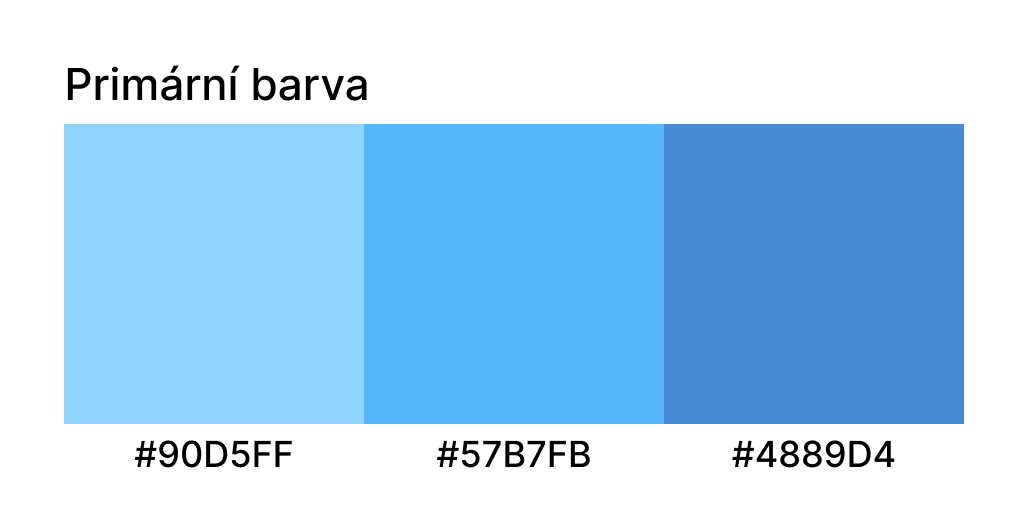
\includegraphics[width=\textwidth]{./images/Primary Color.png}
        \caption{Volba primární barvy}
        \label{fig:primary-color}
    \end{minipage}
\end{figure}

% Final
\subsubsection{Sekundární barva}

% Final
Material Design 2 umožňuje kromě primární barvy také definovat sekundární barvu, která slouží k doplnění primární barvy, vytvoření vizuálního kontrastu a zvýraznění určitých prvků rozhraní. Na rozdíl od primární barvy, která typicky reprezentuje samotnou značku aplikace a je v rozhraní přítomna na většině míst, je sekundární barva používána střídměji a pouze u některých prvků UI. Prakticky se tak využívá například na zvýraznění odkazů, v přepínačích, indikátorech stavů aplikace nebo v tzv. \textit{floating action buttons}. Přestože Material Design 2 definuje tuto sekundární barvu, její volba a použití jsou volitelné. \cite{MaterialDesignColorSystem}

% Final
Při volbě sekundární barvy jsem vycházel z principů teorie barev a ze standardně používaných barevných schémat, která definují rozložení barev na barevném kruhu \cite{FigmaWhatIsColorTheory}. Tato schémata slouží jako praktický nástroj pro posouzení, které barvy se vhodně doplňují tak, aby bylo možné je spolu využít například v uživatelském rozhraní. Na základě těchto schémat je tak možné zvolit sekundární barvu, která bude vhodně doplňovat primární barvu a vytvářet tak vizuálně příjemný vzhled uživatelského rozhraní. Při výběru sekundární barvy jsem volil z následujících schémat.

% Final
\paragraph{Monochromatické schéma} Monochromatické schéma využívá jeden odstín a jeho světlejší či tmavší varianty. V rozhraní obvykle působí klidně a kompaktně. Je také snadné na použití, protože designeři musí pracovat pouze s jedním hlavním odstínem. \cite{FigmaWhatIsColorTheory}

% Final
\paragraph{Analogické schéma} Analogické schéma kombinuje sousední barvy na barevném kruhu. Toto schéma je často možné pozorovat v přírodě, kde se podobné odstíny barev často vyskytují blízko sebe. Výsledkem bývá harmonický, méně kontrastní a přírodně vypadající vzhled. \cite{FigmaColorWheel}

% Final
\paragraph{Komplementární schéma} Komplementární schéma využívá dvojici protilehlých barev na barevném kruhu. Vytváří tak vysoký kontrast, což je přínosné pro uchycení a zaměření pozornosti uživatele na důležité prvky UI. Toto schéma tak umožňuje využití kombinace teplejších a chladnějších odstínů v UI. \cite{FigmaColorWheel}

% Final
\paragraph{Rozděleně komplementární schéma} Rozděleně komplementární schéma vychází z komplementární dvojice odstínů, ale místo přímého protikladu jsou využity dvě sousední barvy k doplňkové barvě. V praxi tak designeři mají možnost využít více barev a paleta tak může působit vyváženěji. \cite{FigmaColorWheel} \cite{FigmaWhatIsColorTheory}

% Final
\paragraph{Triadické schéma} Triadické schéma pracuje se třemi barvami rovnoměrně rozmístěnými na barevném kruhu do tvaru rovnostranného trojúhelníku. Toto schéma může působit živěji a dynamičtěji, nicméně stále je třeba určit, která ze tří barev bude v UI dominantní a které barvy budou používány střídměji. \cite{FigmaColorWheel} 

% Final
\paragraph{Tetradické schéma} Tetradické schéma využívá čtyři barvy, které tvoří na barevném kruhu obdélník, často ve formě dvou komplementárních dvojic. Toto schéma nabízí široké možnosti kombinací, avšak jeho použití v designu UI může být náročné, zejména kvůli udržení konzistence ve využití jednotlivých barev. \cite{FigmaColorWheel}

% Final
\paragraph{Čtvercové schéma} Čtvercové schéma využívá, stejně jako předchozí tetradické schéma, čtyři barvy rozmístěné na barevném kruhu. V tomto schématu jsou ovšem barvy rozmístěny rovnoměrně do tvaru čtverce. Podobně jako tetradické schéma poskytuje čtvercové schéma širší možnosti využití jednotlivých barev, nicméně zvyšuje riziko vizuální roztříštěnosti, pokud nejsou stanovena a dodržována jasná pravidla pro použití jednotlivých barev. Oproti tetradickému schématu umožňuje čtvercové schéma sestavit vyrovnanější vzhled ve srovnání s vysokým kontrastem, který tetradické schéma může vytvářet. \cite{FigmaColorWheel}

% Final
V rámci výběru sekundární barvy jsem se rozhodl využít monochromatické schéma, tedy pracovat primárně s jedním odstínem modré a jeho variantami, a samostatnou sekundární barvu pro rozhraní nedefinovat. Toto rozhodnutí přímo plyne ze stanovených zásad minimalismu a důvěryhodnosti. Díky omezení počtu barev by tak mělo uživatelské rozhraní působit minimalističtěji a mělo by být snazší dodržet konzistentní využití barev napříč návrhem a aplikací. Zároveň, jelikož jsem jako primární barvu zvolil světle modrou, by mělo výsledné rozhraní působit klidným a méně rušivým dojmem \cite{FigmaLightBlue}. To bude podstatné zejména při samotném učení, kdy je uživatel vystaven vyšší kognitivní zátěži a příliš agresivní barvy by pro něj mohly být rozptylující.

% Final
Přestože jsem se rozhodl zvolit monochromatické schéma, a využívat tak hlavně primární barvu, bude aplikace obsahovat řadu dalších barev, které budou používány například pro indikaci stavů v aplikaci. Příkladem toho jsou indikace správných a špatných odpovědí uživatele při učení. Těmto barvám se budu věnovat v následujících sekcích.

% Final
\subsubsection{Stavové barvy}

% Final
Kromě zvolení primární a sekundární barvy je třeba také zvolit barvy pro indikaci různých stavů, které mohou v aplikaci nastat. Tyto barvy budou například použity pro indikaci správných a špatných odpovědí uživatele, nebo pro indikaci chyb a varování v aplikaci. Jako základní odstíny jsem zvolil zelenou pro indikaci úspěšných stavů, oranžovou pro indikaci varování a červenou pro indikaci chyb. Jelikož budou tyto barvy často používány při učení, rozhodl jsem se vybrat pastelové varianty těchto barev, aby působily méně agresivním dojmem. Podobně jako primární barva by tak měly působit klidně, příjemně a neměly by příliš rozptylovat uživatele při učení.

% Final
Podobně jako u primární barvy, umožňuje Material Design 2 definovat hlavní variantu \texttt{main}, světlou variantu \texttt{light} a tmavou variantu \texttt{dark} pro každou barvu. Dále knihovna Material UI umožňuje definovat také odpovídající barvu textu \texttt{contrastText} \cite{MUIPalette}, která je dostatečně kontrastní vůči dané barvě a dodržuje tak standard přístupnosti \textit{Web Content Accessibility Guidelines 2.2}, dále WCAG 2.2 \cite{WCAG22}. Pro každý stav jsem tak vybral varianty barev, jejichž ukázku lze nalézt na obrázku \ref{fig:status-colors}. 

% Final
\begin{figure}[!ht]
    \centering
    \begin{minipage}{0.6\textwidth}
        \centering
        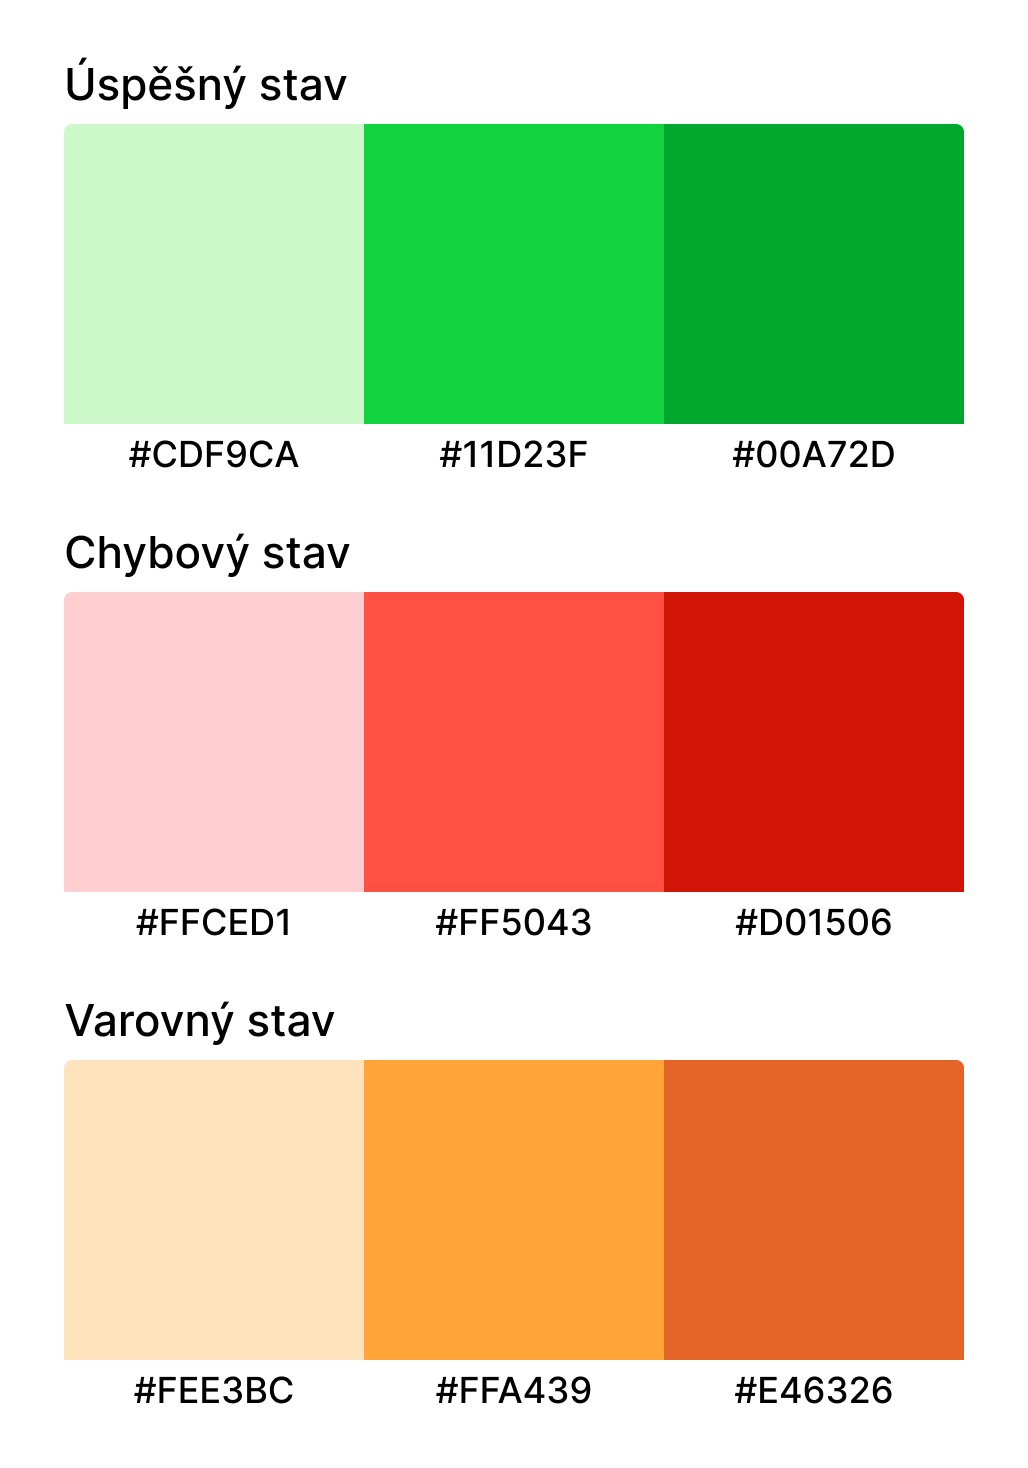
\includegraphics[width=\textwidth]{./images/Status Colors.png}
        \caption{Volba barev pro indikaci stavů}
        \label{fig:status-colors}
    \end{minipage}
\end{figure}

% Final
Podobně jako u primární barvy jsem pro volbu jednotlivých variant využil nástroj Material palette generator.

% Final
\subsubsection{Barvy pozadí}

% Final
Jako barvu pozadí \texttt{background} jsem se rozhodl využít výchozí barvu Material Design 2, tedy bílou barvu \texttt{\#FFFFFF}. Tato barva je používána zejména pro pozadí jednotlivých stránek. Jako barvu povrchů, neboli barvu pozadí některých komponentů, jsem dále zvolil světle šedou barvu \texttt{\#F3F3F3} označovanou jako \texttt{paper}, díky které bude možné komponenty lépe odlišit od pozadí stránek. Tyto barvy budou používány ve světlém režimu aplikace.

% Final
Ukázky barev pozadí a povrchů lze nalézt na obrázku \ref{fig:background-colors}.

% Final
\begin{figure}[!ht]
    \centering
    \begin{minipage}{0.5\textwidth}
        \centering
        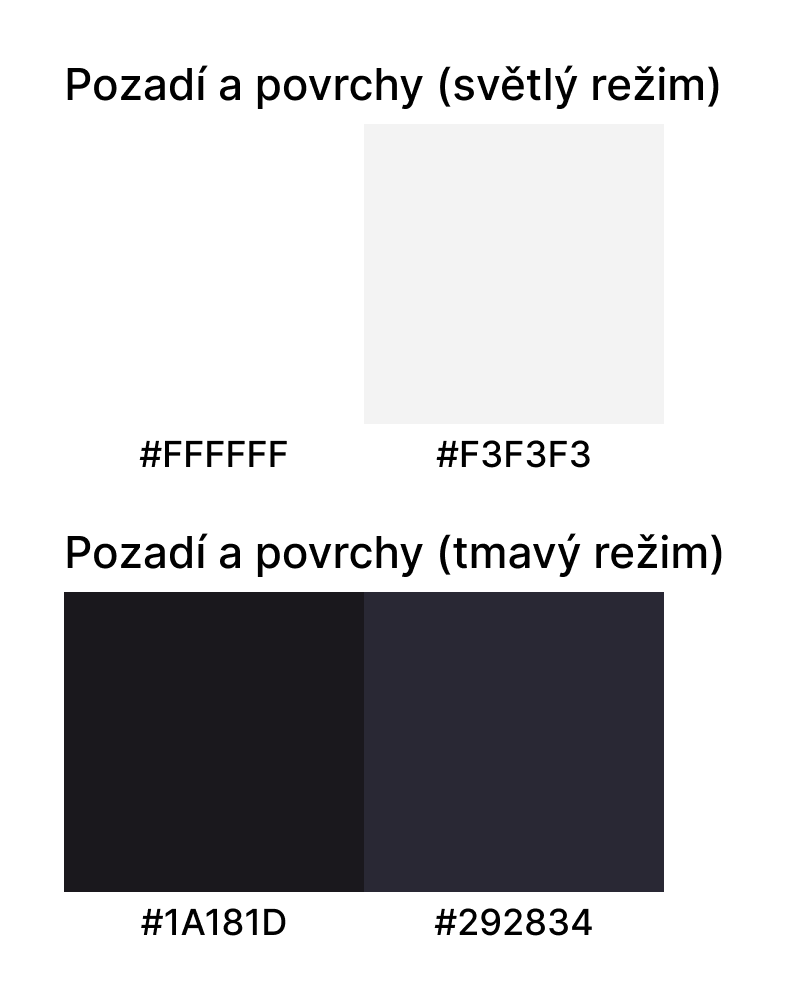
\includegraphics[width=\textwidth]{./images/Background Colors.png}
        \caption{Volba barev pozadí a povrchů}
        \label{fig:background-colors}
    \end{minipage}
\end{figure}

% Final
\subsubsection{Barvy textu}

% Final
Pro textové prvky jsem se rozhodl využít výchozí barvu Material Design 2, tedy černou barvu \texttt{\#000000}. Kromě této primární barvy textu knihovna Material UI ještě umožňuje definovat sekundární barvu textu, kterou je možné využít například pro odstavce a vytvořit tak silnější vizuální kontrast mezi nadpisy a běžným textem. Jako sekundární barvu jsem se tak rozhodl využít barvu \texttt{\#6f6f6f}, která je výrazně světlejší než černá barva, nicméně i pro běžný text stále splňuje kontrastní poměr mezi textem a barvami pozadí 4.5:1 dle AA standardu WCAG 2.2 \cite{WCAG22}.

% Final
\subsubsection{Tmavý režim}

% Final
Jedním z definovaných požadavků je dostupnost tmavého režimu aplikace. Pro vytvoření tmavého režimu je třeba jednotlivé barvy upravit tak, aby je bylo možné využívat na tmavých pozadích a aby stále odpovídaly standardu WCAG 2.2 \cite{WCAG22}. Při tvorbě tmavého režimu jsem postupoval dle doporučení oficiální dokumentace Material Design 2 \cite{MaterialDesign2DarkTheme}.

% Final
Jako první krok jsem se rozhodl zvolit samotné barvy pozadí a povrchů pro tmavý režim. Jako barvu pozadí jsem zvolil tmavě šedou barvu \texttt{\#1A181D} a jako barvu povrchů jsem dále zvolil lehce světlejší šedou barvu \texttt{\#292834}. Hlavním důvodem pro použití tmavě šedých barev, místo čistě černé barvy, je snaha dosáhnout nižšího kontrastu mezi světlým textem a tmavým pozadím. Text je pak lépe čitelný a méně namáhá oči uživatele. \cite{MaterialDesign2DarkTheme}

% Final
Po vybrání barvy pozadí je třeba přizpůsobit saturaci primární barvy, barvy stavů a barvy textu tak, aby byl dodržen kontrastní poměr 4.5:1 mezi textem a tmavým pozadím \cite{WCAG22}. Pro nalezení odpovídajících méně saturovaných barev jsem využil nástroj Colour contrast checker\footnote{Dostupné na: \href{https://colourcontrast.cc/}{https://colourcontrast.cc/}}, který mi umožnil vybrat k jednotlivým barvám jejich méně saturované varianty a zkontrolovat dodržení kontrastního poměru.

% Final
Nakonec jsem vybral barvy textu pro tmavý režim. Jako primární barvu textu jsem zvolil výchozí bílou barvu \texttt{\#FFFFFF} a jako sekundární barvu jsem zvolil \texttt{\#989898}. Obě barvy opět splňují požadovaný kontrastní poměr.

% Final
\subsection{Typografie}

% Final
V této sekci se zaměřím na volbu písma. Podobně jako u volby palety barev budu vycházet ze standardu Material Design 2 a budu volit vlastnosti písma v souladu se standardem přístupnosti WCAG 2.2 \cite{WCAG22}.

% Final
\subsubsection{Výběr písma}

% Final
Jako základní písmo jsem se rozhodl využít rodinu písem Inter\footnote{Dostupné na: \href{https://rsms.me/inter/}{https://rsms.me/inter/}}. Tato rodina písem byla publikována v roce 2017, zaměřuje se na moderní a čistý vzhled, podporuje přes 147 jazyků a je široce využívána napříč různými obory. Pro tuto rodinu písem jsem se rozhodl zejména z důvodu moderního a profesionálního vzhledu a její široké podpory a rozšířenosti. \cite{Inter}

% Final
Při volbě písma je možné dále využít tzv. párování fontů \cite[271-272]{Tidwell2020DesigningInterfaces}, při kterém se pro nadpisy využije jiná rodina písma, než pro běžný text. Díky tomu lze dosáhnout výraznějšího rozlišení mezi nadpisy a běžným textem a také zajímavějšího vzhledu rozhraní. Při tomto párování je ovšem třeba použít písma, která jsou od sebe dostatečně odlišná a využít tak například patková a bezpatková písma. Pro zachování minimalismu jsem se rozhodl toto párování nevyužít a použít tak rodinu písem Inter pro nadpisy i běžný text.

% Final
Dále, jelikož budou v aplikaci často využívány ukázky kódu, bylo potřeba zvolit písmo pro zobrazování kódu. Pro tento účel jsem se rozhodl využít rodinu písem JetBrains Mono\footnote{Dostupné na: \href{https://www.jetbrains.com/lp/mono/}{https://www.jetbrains.com/lp/mono/}}, která je speciálně navržena tak, aby byla dobře použitelná v editorech kódu a aby byl samotný kód dobře čitelný. \cite{JetBrainsMono}

% Final
\subsubsection{Hierarchie a škálování}

% Final
Po výběru rodiny písma je třeba dále zvolit typografickou škálu, která bude určovat velikosti jednotlivých textových prvků rozhraní, jako například velikosti nadpisů, podnadpisů a odstavců. Prvním krokem při volbě škály je zvolení základní velikosti písma, například 16 pixelů. Tato velikost reprezentuje velikost běžného textu v odstavcích. Následně se, na základě zvolené škály, toto číslo násobí daným poměrem, čímž se získají velikosti nadpisů, podnadpisů a dalších textových prvků.

% Final
Volba typografické škály tak určuje, jaký je rozdíl mezi velikostmi jednotlivých textových prvků. Tento rozdíl pak ovlivňuje, jak velký bude vizuální kontrast mezi jednotlivými prvky. Škály s vysokým kontrastem, jako například \textit{Golden ratio} s poměrem 1,618, jsou vhodné pro velké obrazovky \cite{TypographicScales}. Naopak škály s nízkým kontrastem, jako například \textit{Major Second} s poměrem 1,125, umožňují zobrazit větší množství textu na jedné stránce, jelikož jednotlivé textové prvky nezabírají tolik prostoru. Takové škály se často používají například na mobilních zařízeních, kde je prostor na obrazovce omezený.

% Final
Při volbě škály jsem nejprve použil oficiální nástroj pro generaci typografické škály dle standardu Material Design 2 \cite{MaterialDesign2TypeSystem}. Po aplikaci této škály při návrhu uživatelského rozhraní jsem ovšem došel k názoru, že tato škála vytváří příliš vysoký kontrast mezi textovými prvky. Velké nadpisy zabíraly příliš mnoho prostoru a byly při návrhu rozhraní pro tento typ aplikace takřka nepoužitelné. Nedostatek menších nadpisů tak neumožňoval dosáhnout detailnějšího odlišení jednotlivých sekcí a podsekcí v aplikaci, což značně znepřehledňovalo například stránky se cvičeními a vysvětlením látky. Došel jsem tak k závěru, že výchozí typografická škála Material Design 2 není pro tuto aplikaci vhodná.

% Final
Z tohoto důvodu jsem se rozhodl zvolit vlastní typografickou škálu, která bude vhodnější pro tento typ aplikace. Rozhodl jsem se vybrat dvě škály, jednu pro mobilní zařízení a jednu pro desktopová zařízení. Pro mobilní zařízení jsem se rozhodl využít škálu s nižším kontrastem \textit{Minor Third} s poměrem 1.200 a pro desktopová zařízení škálu \textit{Major Third} s poměrem 1,250. Díky těmto škálám tak bude možné plně využít všechny velikosti nadpisů a text tak bude lépe přizpůsoben velikostem jednotlivých zařízení. \cite{TypographicScales}

% Final
Pro generaci konkrétních velikostí písma jsem následně využil nástroj Typescale\footnote{Dostupné na: \href{https://typescale.com/}{https://typescale.com/}}. Při aplikaci vygenerované škály v návrhu rozhraní jsem následně dodržoval standardy Material Design 2, které se týkají vlastností jednotlivých textových prvků a definují například doporučené rozmezí velikostí písma.

% Final
\subsection{Ikony a ilustrace}

% Final
V rámci návrhu rozhraní je dále třeba zvolit vhodnou kolekci ikon a ilustrací. Pro vzhled ikon jsem se rozhodl využít kolekci Material Icons\footnote{Dostupné na: \href{https://fonts.google.com/icons}{https://fonts.google.com/icons}}. Pro návrh jsem se rozhodl využít zaoblenou variantu těchto ikon, aby rozhraní působilo hravějším a zábavnějším dojmem.

% Final
Jelikož bude aplikace obsahovat různé formy gamifikace a další motivační prvky, je třeba do návrhu zahrnout, kromě základních ikon, i různé ilustrace. Jako zdroj ilustrací jsem se rozhodl využít repozitář ilustrací publikovaných pod svobodnými licencemi SVG Repo\footnote{Dostupné na: \href{https://www.svgrepo.com/}{https://www.svgrepo.com/}}. Jednotlivé ilustrace jsem se pak snažil volit tak, aby měly vzájemně konzistentní styl.

% Final
\subsection{Animace a zvukové efekty}

% Final
V rámci návrhu jsem se dále rozhodl, v souladu s nefunkčními požadavky, navrhnout i animace a efekty, které by měly být při implementaci použity. Příslušné animace a efekty jsem vyznačil poznámkami u jednotlivých stránek v návrhu uživatelského rozhraní.

% Final
Mezi použité animace patří například animace přechodu mezi stránkami, animace zmáčknutí tlačítka, animace konfet při dokončení lekce, animace indikátoru pokroku při učení a další.

% Final
Kuriozitou při návrhu rozhraní bylo využití zvukových efektů. Zvukové efekty bývají ve webových aplikacích využívány velice zřídka, zejména kvůli tomu, že často nejsou pro interakci s uživatelem potřeba a zbytečně by uživatele rušily při práci s aplikací. V jistých případech mohou být ovšem zvukové efekty vhodné pro podpoření určitých emocí u uživatele a pro zvýšení intenzity požitku z vykonání určitých akcí. V této aplikaci tak budu využívat zvukové efekty například při samotném učení uživatele pro indikaci správných a špatných odpovědí nebo při úspěšném dokončení lekce. Jako zdroj zvukových efektů jsem se rozhodl využít soubor efektů Material Product Sounds\footnote{Dostupné na: \href{https://m2.material.io/design/sound/sound-resources.html}{https://m2.material.io/design/sound/sound-resources.html}}. Podobně jako u animací jsem vyznačil zvukové efekty v návrhu uživatelského rozhraní na místech, kde by měly být použity. \cite {MaterialDesign2ApplyingSounds}

% Final
\section{Návrh prototypu uživatelského rozhraní}

% Final
V této sekci se zaměřím na návrh \textit{high fidelity} prototypu uživatelského rozhraní\footnote{Dostupné na: \href{https://www.figma.com/design/VZFuqWojrXq8yWjrBIq4OH}{https://www.figma.com/design/VZFuqWojrXq8yWjrBIq4OH}}, tedy prototypu, který bude obsahovat detailní návrh uživatelského rozhraní včetně definovaných stylů, barev, písma, ilustrací a interakcí \cite[53-54]{NURUIDesignSteps}. Cílem je tak vytvořit návrh uživatelského rozhraní, které bude přesně specifikovat vzhled aplikace a přechody mezi jednotlivými stránkami. Prototyp následně bude sloužit jako podklad pro samotnou implementaci aplikace.

% Final
Pro tvorbu prototypu jsem zvolil nástroj Figma\footnote{Dostupné na: \href{https://www.figma.com/}{https://www.figma.com/}}, protože umožňuje rychlé iterace návrhu, práci s komponentami a také propojení obrazovek do podoby interaktivního prototypu. Při návrhu jsem vycházel ze stylů definovaných v předchozí sekci.

% Final
\subsection{Tvorba prototypu}

% Final
V rámci mé bakalářské práce jsem se mimo jiné věnoval vytvoření návrhu uživatelského rozhraní pro původní aplikaci na výuku angličtiny \cite{Jenicek2024BachelorThesis}. V průběhu let jsem ovšem zpozoroval několik nedostatků tohoto prototypu. Použitá knihovna předdefinovaných komponentů je zbytečně složitá a komplikuje vytváření a používání nových komponentů. Prototyp také nevyužívá moderní funkce programu Figma, jako například definice globálních proměnných a proměnných komponentů. S ohledem na nově definované styly, nové funkce a na nový účel aplikace jsem se tak rozhodl vytvořit celý návrh uživatelského rozhraní od začátku a bez návaznosti na původní prototyp.

% Final
Při tvorbě prototypu jsem postupoval následovně. Nejprve jsem pomocí proměnných zadefinoval jednotlivé styly aplikace dle návrhu popsaného v předchozí sekci. Následně jsem provedl hrubý návrh základních komponent a stránek aplikace. Poté jsem se v rámci agilního procesu vývoje vždy zaměřil na jednu funkci, kterou jsem navrhl podrobněji a zprovoznil její interakce v prototypu. Po dokončení návrhu dané funkce jsem provedl její implementaci a testování, které jsou popsané v následujících kapitolách. Po dokončení dané funkce jsem se přesunul na následující funkci, dle její priority. Po dokončení návrhu všech funkcí jsem provedl závěrečné úpravy návrhu a organizaci jednotlivých stránek a komponentů.

% Final
Při návrhu jsem kladl důraz na znovupoužitelnost komponentů a na využití pokročilejších možností programu Figma, díky kterým bude možné prototyp v budoucnu jednodušeji rozšiřovat a upravovat. Konkrétně jsem široce využíval komponenty a jejich varianty, díky kterým je zajištěna vyšší konzistence samotného návrhu. Dále jsem využíval lokální proměnné komponentů a globální kolekce proměnných, díky kterým je možné kdykoliv měnit styly v celém návrhu, aniž by bylo nutné modifikovat samotné stránky a komponenty \cite{FigmaVariablesGuide}. 

% Final
Jednotlivé komponenty jsem dále strukturoval tak, aby bylo možné je přímo implementovat s využitím jejich zadefinovaných parametrů v prototypu. Při návrhu jsem také často využíval funkci \textit{auto layout}, díky které je možné přesně specifikovat rozložení komponentů tak, aby byly responzivní a použitelné v různých částech UI \cite{FigmaAutolayoutGuide}.

% Final
Jako součást návrhu jsem také vytvořil dva režimy rozhraní aplikace, světlý a tmavý. Oba režimy sdílí stejné rozvržení stránek a komponentů a liší se pouze aplikovanými styly, zejména barvami pozadí, textu a stavů. Pro definici světlého a tmavého režimu jsem využil funkci módů proměnných \cite{FigmaModesForVariables}, díky které je možné pro každý režim definovat jiné hodnoty proměnných a následně snadno mezi jednotlivými režimy přepínat. Díky tomu byla opět zajištěna vyšší konzistence návrhu, jelikož není třeba pro světlý a tmavý režim navrhovat samostatné stránky, ale je možné pouze přepínat mezi aplikovanými styly.

% Final
Vytvořený návrh vzhledu jsem také doplnil o interakce odpovídající reálnému používání aplikace. Zaměřil jsem se zejména na navigaci mezi obrazovkami tak, aby bylo možné procházet základní scénáře používání aplikace. Díky tomu bylo možné prototyp interaktivně procházet, což mi umožnilo odhalit různé nedostatky v návrhu ještě před zahájením implementace.

% Final
Pro ukázku návrhu jsem vybral několik stránek z prototypu. Tyto stránky lze nalézt na obrázcích \ref{fig:navrh-1}, \ref{fig:navrh-2}, \ref{fig:navrh-3} a \ref{fig:navrh-4}.

% Review
\begin{figure}[!ht]
    \centering
    \begin{minipage}{0.45\textwidth}
        \centering
        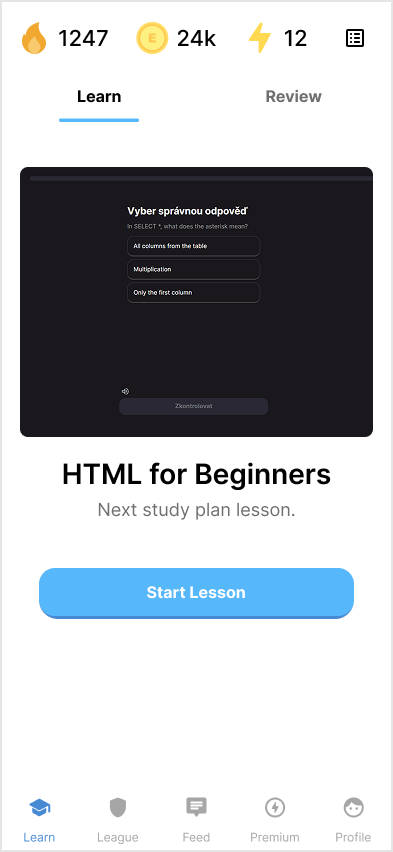
\includegraphics[width=\textwidth]{./images/home [learn-section].png}
        \caption{Ukázka návrhu hlavní stránky aplikace}
        \label{fig:navrh-1}
    \end{minipage}
    \hfill
    \begin{minipage}{0.45\textwidth}
        \centering
        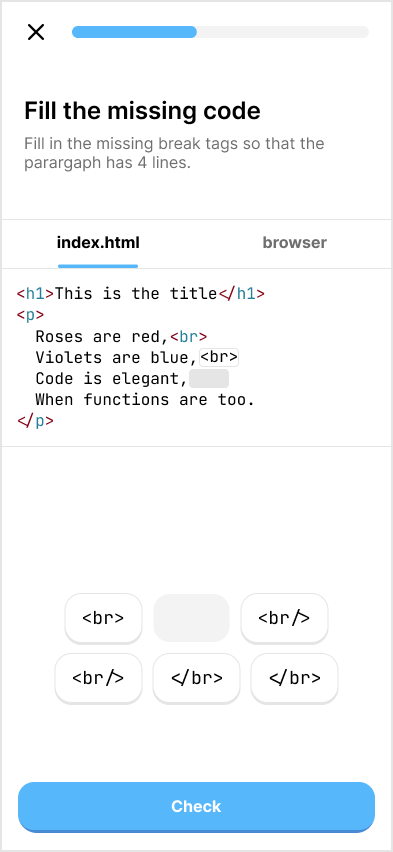
\includegraphics[width=\textwidth]{./images/study-session [fill in code].png}
        \caption{Ukázka návrhu cvičení programování}
        \label{fig:navrh-2}
    \end{minipage}
\end{figure}

% Review
\begin{figure}[!ht]
    \centering
    \begin{minipage}{0.45\textwidth}
        \centering
        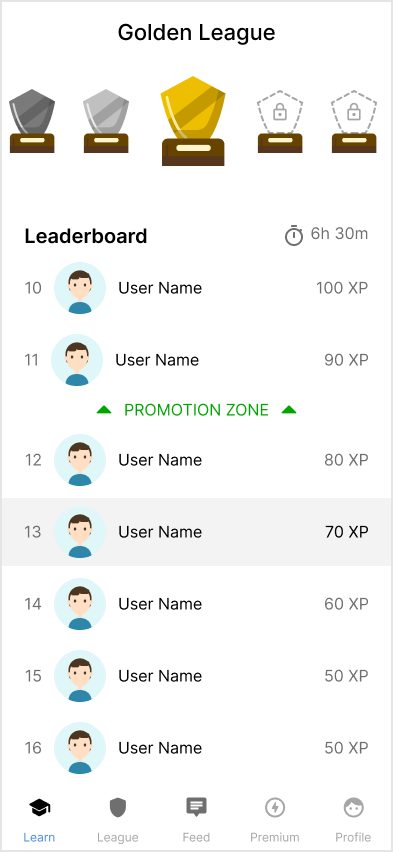
\includegraphics[width=\textwidth]{./images/leaderboard.png}
        \caption{Ukázka návrhu žebříčku uživatelů}
        \label{fig:navrh-3}
    \end{minipage}
    \hfill
    \begin{minipage}{0.45\textwidth}
        \centering
        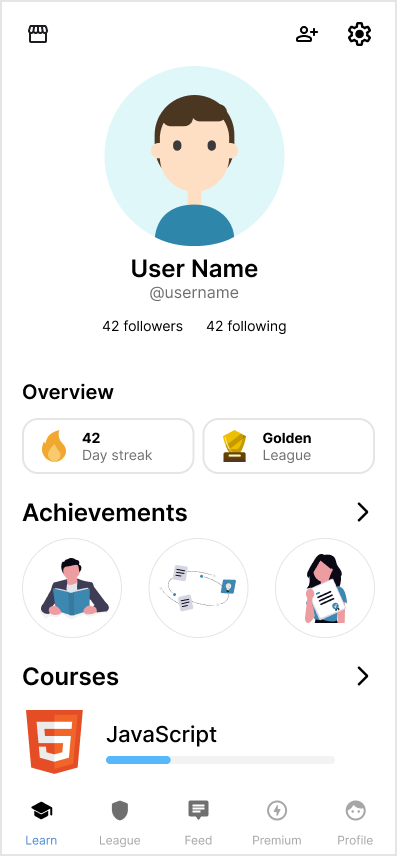
\includegraphics[width=\textwidth]{./images/user.png}
        \caption{Ukázka návrhu uživatelského profilu}
        \label{fig:navrh-4}
    \end{minipage}
\end{figure}

% Final
\subsection{Responzivita}

% Final
Návrh prototypu jsem realizoval přístupem \textit{mobile-first} \cite{MobileFirst}. Primární cílovou platformou této aplikace jsou mobilní zařízení, proto jsem nejprve navrhl vzhled stránek pro menší rozlišení a teprve následně jsem řešil úpravy pro větší displeje. Tento postup mi umožnil soustředit se na efektivní využití prostoru a na jednoduché rozvržení stránek, které je na malých obrazovkách klíčové.

% Final
Při návrhu prototypu bylo třeba rozhodnout, jakým způsobem bude rozhraní responzivní, tedy jak se bude rozložení stránek přizpůsobovat různým velikostem displeje. Při návrhu responzivity je možné využít několik standardních rozložení stránek. 

% Final
Rozložení \textit{mostly fluid} například typicky pracuje s bloky obsahu, které se přesouvají pod sebe se zmenšující se velikostí obrazovky \cite[7]{NURResponsiveDesign}. Dále je možné využít rozložení \textit{column drop}, které využívá několik sloupců s obsahem a se zmenšující se obrazovkou se sloupce opět přesouvají pod sebe \cite[8]{NURResponsiveDesign}. Také je možné využít rozložení \textit{layout shifter}, které představuje nejkomplexnější ze zmíněných přístupů a spočívá v navržení různé struktury stránek pro každou velikost displeje \cite[9]{NURResponsiveDesign}. 

% Final
V tomto projektu jsem se rozhodl využít přístup \textit{tiny tweaks}, který spočívá v uspořádání veškerého obsahu stránky do jediného sloupce a zachování tohoto rozložení stránky napříč všemi zařízeními \cite[10]{NURResponsiveDesign}. Na stránkách jsou tak při změně velikosti displeje provedeny pouze drobné úpravy ve velikostech jednotlivých komponentů. Implementace se tak bude řídit primárně návrhem pro mobilní zařízení a na větších displejích se budou měnit především maximální šířka obsahu, odsazení a práce s volným prostorem. Kromě toho bude struktura stránek zachována a bude napříč zařízeními stejná.

% Final
Jako důsledek zvolení tohoto přístupu je tak možné udržet návrh jednoduchý a konzistentní. Zároveň díky totožnému rozložení stránek je snížené riziko rozdílného chování napříč různými velikostmi displejů. Aplikaci by tak mělo být snazší rozšiřovat, udržovat a testovat.

% Final
\subsection{Testování a upravování prototypu}

% Final
Prototyp jsem průběžně manuálně testoval, upravoval a zdokonaloval. Při testování a procházení prototypu jsem se snažil zachytit základní problémy v použitelnosti a nekonzistenci návrhu a identifikovat tak nedostatky návrhu ještě před samotnou implementací.

% Final
Návrh jsem se pak snažil průběžně upravovat tak, aby lépe odpovídal očekávaným potřebám uživatelů a aby byl v souladu se zavedenými zásadami designu. Při upravování návrhu jsem se zaměřoval zejména na to, aby návrh splňoval 10 základních heuristik použitelnosti UI definovaných Jakobem Nielsenem \cite{Nielsen10Heuristics}. Výsledná aplikace by tak měla být pro uživatele lépe použitelná.

% Final
\section{Návrh architektury aplikace}

% Final
Při návrhu architektury jsem se rozhodl vycházet z architektury původní aplikace. Systém je rozdělen do frontendové a backendové části. Komunikace mezi těmito částmi probíhá prostřednictvím REST API. Dále je v systému zavedený mock API, který simuluje chování REST API a umožňuje tak frontendovou část aplikace testovat a vyvíjet nezávisle na backendové části. Tento přístup jsem se rozhodl zachovat, protože zjednodušuje paralelní vývoj obou částí a umožňuje průběžně testovat chování frontendové části aplikace nezávisle na stavu backendové části. Architektuře backendové části aplikace včetně návrhu API se věnuje kolega Bc. Jakub Vondráček v rámci své diplomové práce.

% Final
Frontendová část je tvořena webovou aplikací postavenou na frameworku Next.js. Oproti původní aplikaci jsem se rozhodl do systému zavést oddělené knihovny komponentů \texttt{@eduriam/ui-core} a \texttt{@eduriam/ui-x}. Knihovna \texttt{@eduriam/ui-core} bude obsahovat základní komponenty uživatelského rozhraní, zatímco knihovna \texttt{@eduriam/ui-x} bude obsahovat komplexnější komponenty využívané zejména ve výukových částech aplikace. Cílem tohoto rozdělení je oddělit obecně použitelné UI komponenty od aplikační logiky a umožnit tak jejich opětovné využití v různých částech projektu.

% Final
Kromě těchto hlavních částí dále existuje webová stránka aplikace a systém pro správu obsahu aplikace. Tyto části systému nejsou součástí této práce, nicméně budou využívat zmíněné knihovny komponentů, a je tak nutné tyto části zohlednit při návrhu architektury. Přehled architektury aplikace z pohledu frontendu je znázorněn na obrázku \ref{fig:architecture}.

% Final
\begin{figure}[!h]
    \centering
    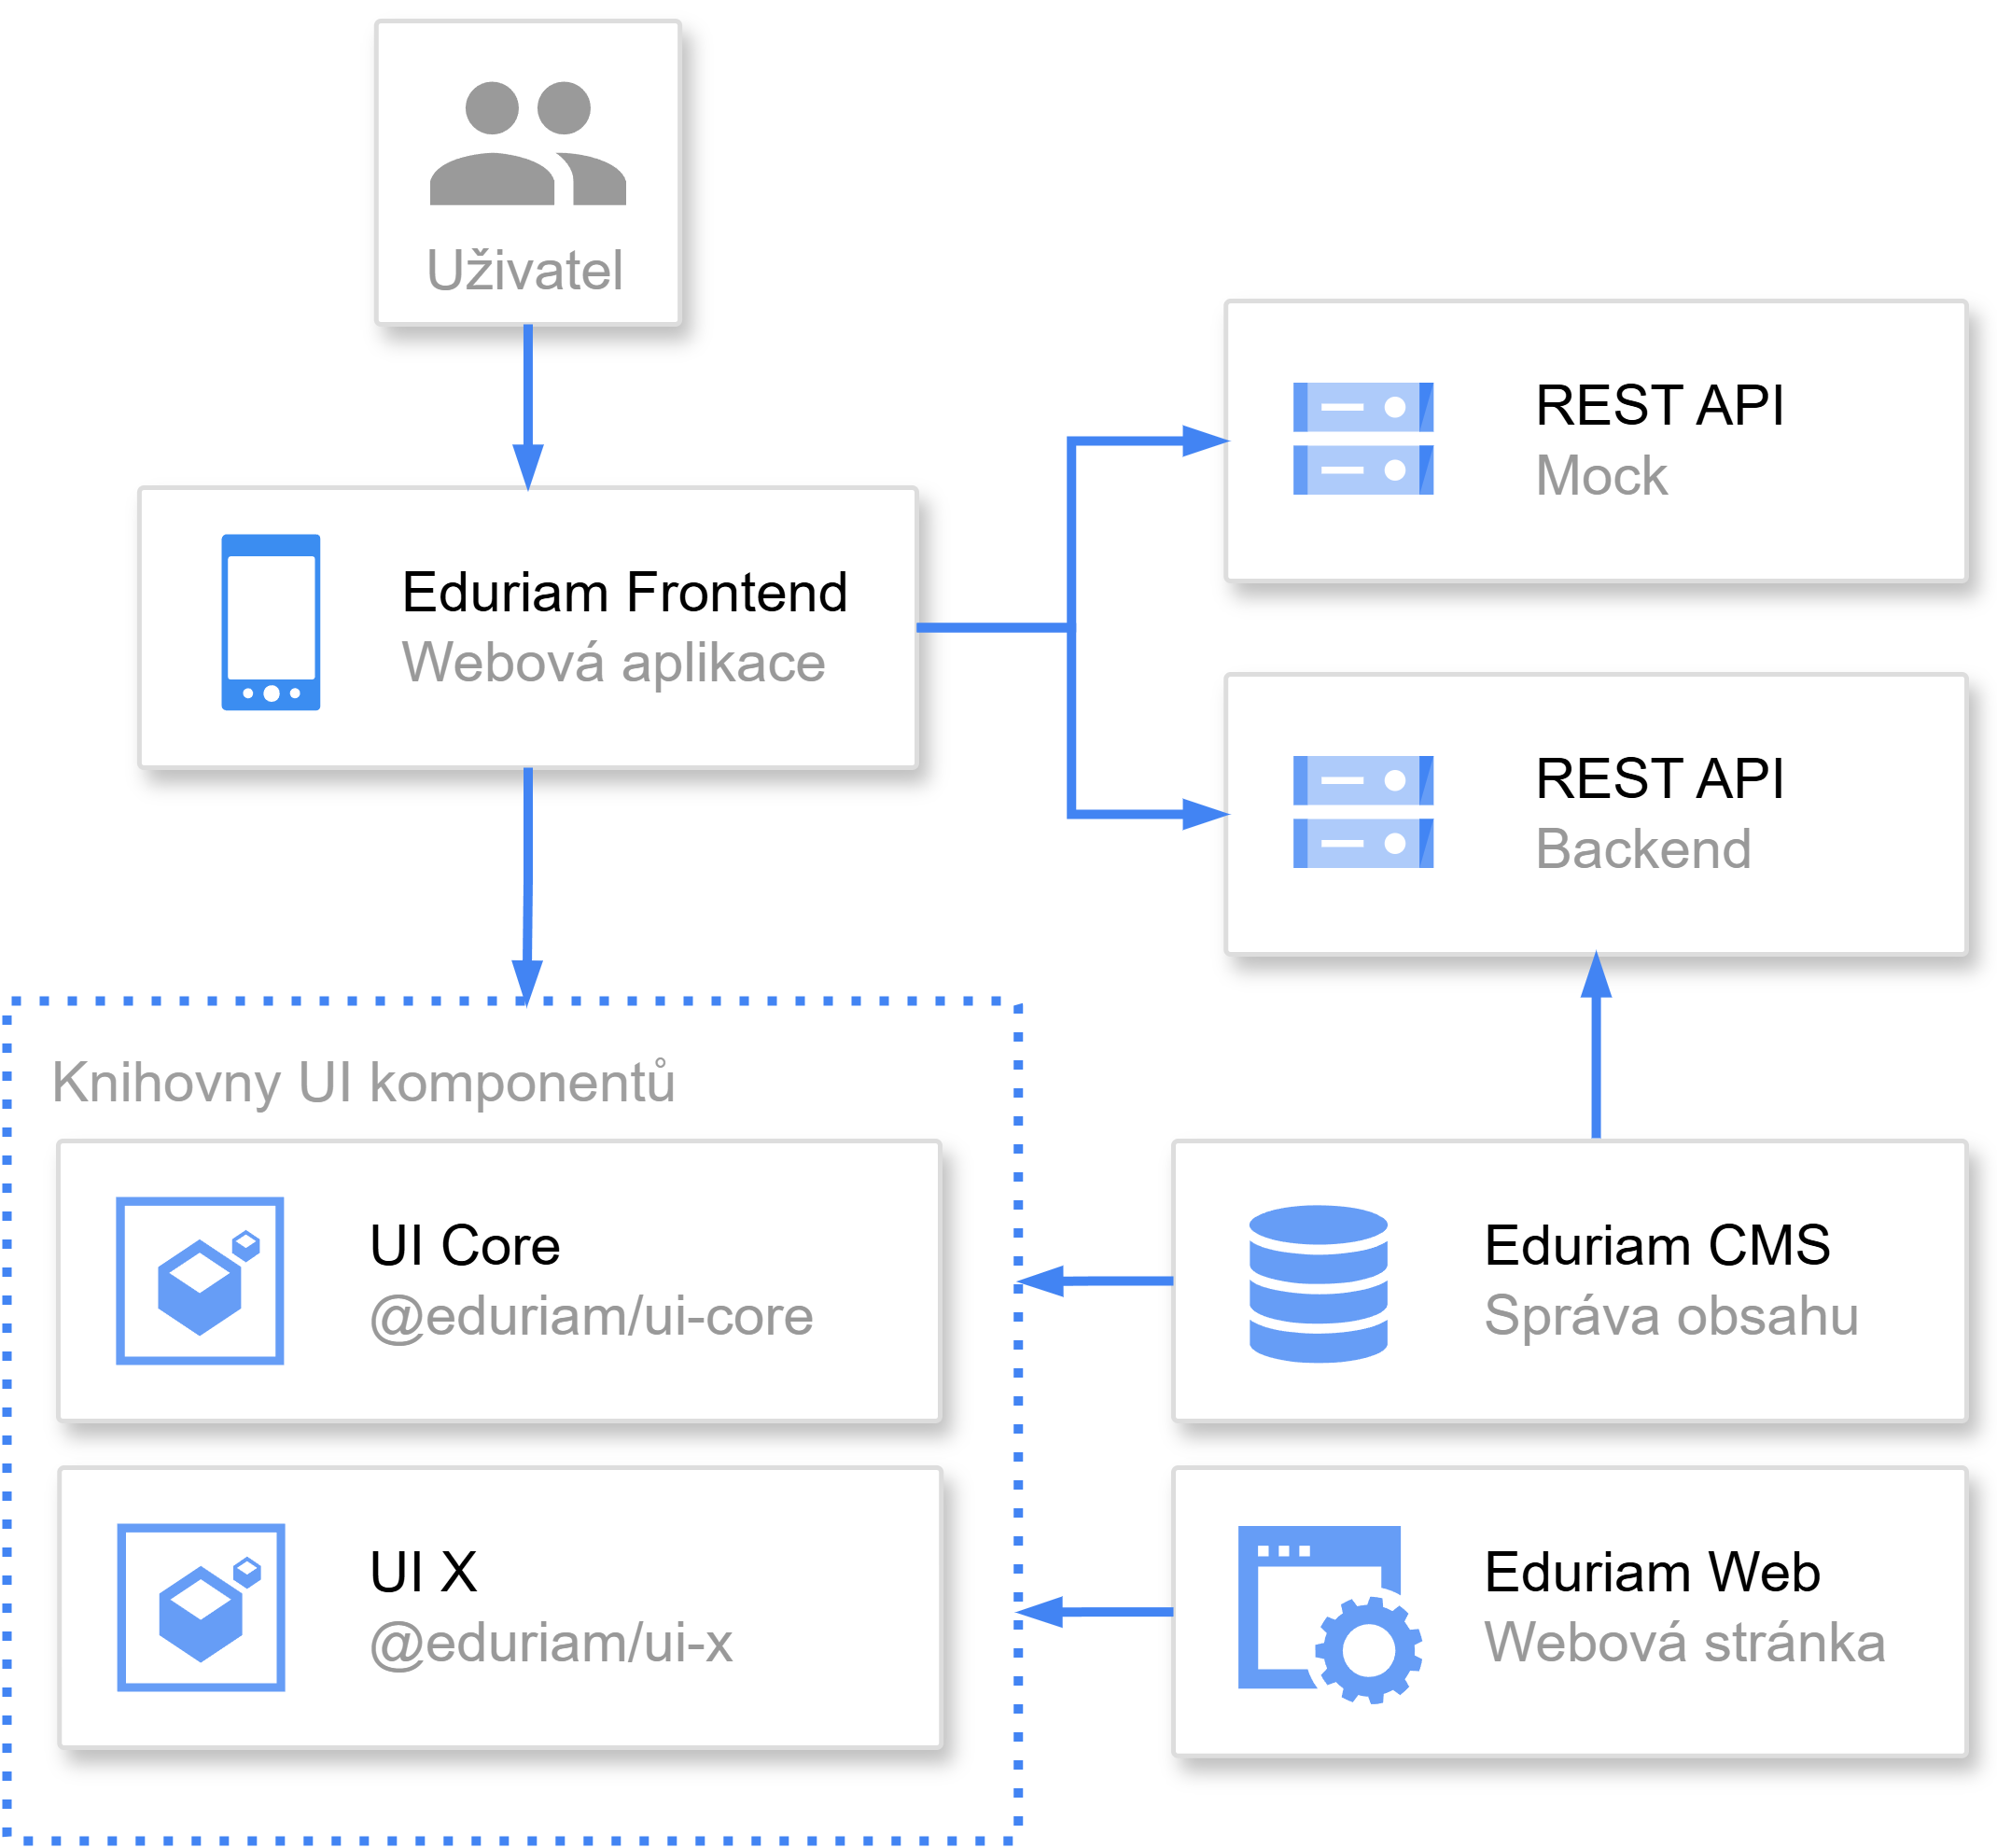
\includegraphics[width=\textwidth]{./images/diagrams/architecture.png}
    \caption{Základní návrh architektury aplikace}
    \label{fig:architecture}
\end{figure}


% Chapter: Implementation
% Final
\chapter{Implementace a nasazení}

% Final
V předchozích kapitolách jsem se věnoval analýze a návrhu jednotlivých částí aplikace. V této kapitole navážu na předchozí kapitoly a popíšu, jakým způsobem jsem postupoval při implementaci a nasazení aplikace.

% Final
Nejprve se zaměřím na úvodní úpravy aplikace, které jsem provedl s cílem připravit aplikaci na nadcházející vývoj. Tyto úpravy se týkaly zejména aktualizace používaných knihoven, aktualizace konvencí a linterů, refaktoringu kódu a zavedení nástrojů umělé inteligence pro asistenci při vývoji.

% Final
Dále popíšu, jakým způsobem jsem postupoval při vývoji a jakým způsobem jsem spolupracoval s kolegou Bc. Jakubem Vondráčkem, který se v rámci jeho diplomové práce věnuje backendové části této aplikace.

% Final - tady kdyžtak upravit pokud bych nedělal nějakou tu podkapitolu
Dále podrobněji popíšu implementaci vybraných funkcí aplikace. Mezi tyto funkce patří například nová struktura učení, systém notifikací, autentizace pomocí účtu Google nebo přizpůsobení aplikace tak, aby splňovala požadavky progresivních webových aplikací a bylo ji tak možné stáhnout a nainstalovat na zařízení uživatele.

% Final
Nakonec popíšu, jakým způsobem jsem nasadil frontendovou část aplikace do jednotlivých prostředí. Nejprve popíšu testovací prostředí, ve kterém aplikace využívá mock API. Tento mock simuluje reálné API a umožňuje tak testování nezávisle na stavu backendové části aplikace. Dále popíšu druhé testovací prostředí, ve kterém aplikace využívá backendové API nasazené v testovacím režimu. Nakonec popíšu nasazení do produkčního prostředí, ve kterém aplikace využívá produkční verzi backendového API. Věnovat se budu také nasazení knihoven, které jsem vytvořil v rámci vývoje této aplikace.

% Final
\section{Postup při realizaci projektu}

% Final
V této části textu nejprve popíšu úvodní přípravu projektu a jednotlivé kroky, které jsem provedl před zahájením implementace. Následně popíšu, jakým způsobem jsem postupoval při samotné implementaci a jak jsem spolupracoval s kolegou Bc. Jakubem Vondráčkem, který se zabývá backendovou částí této aplikace.

% Final
\subsection{Příprava implementace}

% Final
Před zahájením samotné implementace bylo třeba provést úvodní přípravu projektu. Tuto přípravu bylo třeba provést hned z několika důvodů. Původní aplikace byla naposledy aktivně vyvíjena v roce 2024, kdy jsem ji společně s kolegou Bc. Janem Hlaváčem vyvíjel v rámci našich bakalářských prací. Přestože jsme se projektu věnovali i po dokončení bakalářských prací, naše zaměření bylo především na části projektu které se netýkaly samotného vývoje. Vývoj tak ustál a aplikace nedostávala žádné nové aktualizace. Od roku 2024 došlo k řadě změn, kterým je nyní třeba projekt přizpůsobit.

% Final
První změnou jsou nové verze používaných knihoven. Většina používaných knihoven od posledního vývoje vydala nové verze, které obsahují podstatné opravy a vylepšení. Jejich aktualizace tak mohou přinést řadu výhod, jako například nové funkce, efektivnější vývoj, větší bezpečnost a stabilitu funkcí.

% Final
Další zásadní změnou je nástup nástrojů umělé inteligence v oblasti softwarového inženýrství. Tyto nástroje zásadně mění, jakým způsobem lze postupovat při vývoji softwaru a umožňují vyvíjet aplikace efektivnějším způsobem. Proto je třeba projekt přizpůsobit tak, aby byl připraven pro práci s těmito nástroji.

% Final
Nakonec, došlo k zásadní změně domény, na kterou se tato vzdělávací aplikace zaměřuje. Původní aplikace byla zaměřena výhradně na výuku jazyků. Nová aplikace by měla fungovat jako obecnější rozšiřitelná vzdělávací aplikace se zaměřením na výuku programování. Z tohoto důvodu je třeba změnit strukturu některých částí aplikace tak, aby bylo možné ji v budoucnu lépe rozšiřovat a udržovat. Se změnou domény se také pojí odstranění některých zastaralých funkcí, které neodpovídají novému zaměření aplikace.

% Final
V následujících částech textu tak podrobněji popíšu jednotlivé kroky přípravy projektu. Tuto přípravu jsem prováděl současně s předchozími fázemi analýzy a návrhu.

% Final
\subsubsection{Příprava knihoven komponentů}

% Final
V rámci přípravy aplikace jsem se rozhodl od aplikace oddělit některé UI komponenty a přesunout je do samostatných knihoven, které bude tato aplikace využívat. Komponenty jsem rozdělil do dvou knihoven \texttt{@eduriam/ui-core} a \texttt{@eduriam/ui-x}. První zmíněná knihovna bude obsahovat základní UI komponenty, jako tlačítka, textová pole, karty apod. Druhá zmíněná knihovna pak bude obsahovat komplexnější komponenty, které budou využívány jen ve specifických případech. Toto rozdělení tak reflektuje strukturu knihovny Material UI \cite{MaterialUI}, která je podobně rozdělena na knihovnu základních komponentů MUI Core a na knihovnu komplexnějších komponentů MUI X.

% Final
Důvodů pro rozdělení aplikace do knihoven je hned několik. Vytvoření knihovny \texttt{@eduriam/ui-core} umožní postupně vytvořit jednotný design systém a knihovnu základních komponentů, kterou bude možné využívat jak v samotné aplikaci, tak v dalších částech projektu, jako například na webových stránkách, nebo v dalších interních programech. Díky tomu bude možné dodržet konzistentní design napříč všemi částmi projektu. Dalším důvodem je dodržení design principu \textit{Separation of Concerns} \cite[36]{ADPArchitectures}, který říká, že bychom při vytváření systémů měli jasně oddělit zodpovědnosti jednotlivých částí systému. Díky tomu bude možné docílit přehlednější struktury kódu a lepší testovatelnosti a udržitelnosti celého systému. V případě této aplikace jsem se tak snažil oddělit základní UI komponenty od logiky samotné aplikace.

% Final
Cílem zmíněné knihovny tak bylo oddělit základní UI komponenty od zbytku projektu. Kromě základních komponentů ovšem vznikla potřeba sdílet určité složitější komponenty napříč různými částmi projektu. Zejména se jedná o komponenty, které vizualizují průběh učení dané lekce, tedy komponenty zobrazující jednotlivá cvičení a vysvětlení látky. Tyto komponenty budou využívány jednak v samotné aplikaci a jednak v interním nástroji pro tvorbu obsahu, ve kterém bude možné například zobrazit náhled učení dané lekce. Zmíněný nástroj již není součástí této práce. Jelikož bude knihovna \texttt{@eduriam/ui-core} se základními komponenty využívána ve více programech, snažil jsem se tuto knihovnu zachovat co nejjednodušší a nejmenší. Z tohoto důvodu jsem pro komplexnější komponenty vytvořil samostatnou knihovnu \texttt{@eduriam/ui-x}, kterou bude možné využít v programech, ve kterých budou tyto specifické komponenty skutečně potřeba.

% Final
Další výhodou tohoto přístupu je možnost verzování knihoven pomocí sémantického verzování \cite{SemVer}. Díky tomuto způsobu verzování je možné snadno rozšiřovat a vylepšovat komponenty nezávisle na ostatních částech systému. Knihovny je pak možné postupně aktualizovat a zavádět jejich nové verze do jednotlivých částí projektu. Celý vývoj komponentů je tak strukturovanější a přehlednější.

% Final
Frontend aplikace tak bude využívat obě zmíněné knihovny. Do obou knihoven jsem také zavedl nástroj Storybook\footnote{Dostupné na: \href{https://storybook.js.org/}{https://storybook.js.org/}}, který umožňuje snadno vyvíjet, dokumentovat a testovat UI komponenty v izolovaném prostředí.

% Final
\subsubsection{Aktualizace knihoven a nástrojů}

% Final
Dalším krokem přípravy aplikace byla aktualizace používaných knihoven. Jak jsem již zmínil, v průběhu let byla vydána řada nových verzí používaných knihoven, které mohou přinést řadu dříve zmíněných výhod. Proto jsem se rozhodl aktualizovat nejpodstatnější knihovny a nástroje, které aplikace využívá.

% Final
Mezi aktualizované knihovny patří například Next.js, Material UI, Storybook, ESLint, Prettier, Yarn, Node.js a další. Kromě těchto knihoven jsem dále v průběhu vývoje aktualizoval knihovny, u kterých bylo třeba přejít na jejich novější verze.

% Final
Celkově aktualizace knihoven skutečně přinesla několik výhod. Nejnovější verze knihoven zefektivnily vývoj aplikace, což bylo možné pozorovat například u nástroje Storybook, jehož novější verze přinesla přehlednější a výrazně rychlejší tvorbu UI komponentů díky novým konvencím a rychlejšímu sestavování jednotlivých komponentů při spouštění Storybook serveru.

% Final
\subsubsection{Refaktoring kódu}

% Final
Po aktualizaci knihoven jsem dále provedl refaktoring stávajícího kódu. Nejprve jsem provedl úvodní refaktoring před fází implementace, který se týkal zejména přesunu příslušných komponentů do dříve zmíněných knihoven \texttt{@eduriam/ui-core} a \texttt{@eduriam/ui-x}. Úvodní refaktoring dále zahrnoval zásadní změnu struktury komponentů pro učení, v rámci které jsem komponenty změnil tak, aby byly rozšiřitelnější a lépe udržovatelné. Komponenty jsem tak připravil pro budoucí úpravy a vývoj.

% Final
V rámci úvodního refaktoringu jsem dále vytvořil několik nových komponentů, které usnadňují vývoj a sjednocují rozložení prvků UI na jednotlivých stránkách aplikace. Mezi tyto komponenty patří například \texttt{PageRoot}, \texttt{ContentContainer} a \texttt{PageNavigation}, díky kterým jsou rozložení prvků a navigace napříč stránkami aplikace konzistentní a snadněji konfigurovatelné.

% Final
V průběhu vývoje jsem pak průběžně prováděl další refaktoring, který se týkal zejména odstraňování a aktualizace zastaralých komponentů a stránek. Tyto změny jsem prováděl průběžně zejména kvůli tomu, že bylo snazší staré funkce postupně nahrazovat novými a aktualizovat je, než všechny odstranit najednou.

% Final
\subsubsection{Aktualizace linterů a konvencí}

% Final
V rámci úvodní přípravy projektu jsem také provedl aktualizaci konfigurací nástrojů pro formátování a kontrolu kvality kódu ESLint a Prettier. Jak jsem již zmínil výše, tyto nástroje jsem aktualizoval na jejich novější verze a dále jsem zavedl přísnější pravidla pro kontrolu kódu. Jedním z nově zavedených pravidel je například pravidlo \texttt{eqeqeq}\footnote{Dokumentace dostupná na: \href{https://eslint.org/docs/latest/rules/eqeqeq}{https://eslint.org/docs/latest/rules/eqeqeq}}, které vynucuje používání typově bezpečného porovnávání hodnot pomocí \texttt{===} a \texttt{!==} namísto porovnávání pomocí \texttt{==} a \texttt{!=}.

% Final
Zmíněná pravidla jsem zavedl s cílem snížit riziko vzniku nejednoznačného kódu a chyb, které mohou nastávat při nesprávném použití jazyků JavaScript a TypeScript, ve kterých je frontendová část aplikace naprogramována.

% Final
\subsubsection{Zavedení nástrojů umělé inteligence}

% Final
Další částí přípravy bylo zavedení konvencí pro nástroje umělé inteligence, které mohou vývojářům pomoci s vytvářením kódu. Vycházel jsem ze standardu Agent Skills\footnote{Dostupné na: \href{https://agentskills.io/}{https://agentskills.io/}} definovaným společností Anthropic. Tento standard umožňuje s pomocí souborů ve formátu Markdown definovat instrukce a pravidla pro AI agenty, kteří na základě nich mohou v kódu vykonávat různé úkony. \cite{AgentSkills}

% Final
Zadefinoval jsem tak pravidla a instrukce pro tvorbu nových UI komponentů, nových stránek aplikace, tvorbu automatizovaných testů a práci s \texttt{.feature} soubory, ve kterých jsou definované funkce aplikace.

% Final
Výhodou využití zmíněného standardu je vysoká kompatibilita s nejpoužívanějšími nástroji umělé inteligence pro tvorbu kódu, kterými jsou například Claude Code, Cursor, Codex, Gemini CLI a další. Instrukce tak bude možné využívat napříč různými IDE, nástroji a AI modely. \cite{AgentSkills}

% Final
\subsubsection{Příprava nového návrhu v nástroji Figma}

% Final
V rámci úvodních příprav projektu, které probíhaly současně s analýzou a návrhem, jsem se rozhodl změnit způsob, kterým je tvořen návrh uživatelského rozhraní v nástroji Figma. Návrh uživatelského rozhraní původní aplikace, který jsem vytvořil v rámci mé bakalářské práce, využíval externí knihovnu základních komponentů, které jsem upravil a následně využil v návrhu jednotlivých stránek aplikace.

% Final
Využití knihovny s již připravenými komponenty zpočátku umožnilo rychle a efektivně vytvořit základní prototyp uživatelského rozhraní. Časem se však ukázalo, že má tento přístup zásadní nevýhody při tvorbě \textit{high fidelity} prototypu. Komponenty externí knihovny často využívaly jinou strukturu a parametry, než bylo při návrhu aplikace potřeba. Struktura komponentů a jejich parametrů se tak postupnými úpravami stávala zbytečně složitou, což značně snižovalo efektivitu tvorby prototypu.

% Final
Jelikož mám v rámci této práce za cíl vytvořit kompletně nový a propracovanější vzhled všech komponentů a stránek aplikace, rozhodl jsem se zmíněný přístup změnit a místo externí knihovny komponentů vytvořit všechny komponenty ručně. Díky tomu jsem získal vyšší kontrolu nad tvorbou jednotlivých komponentů a byl jsem schopen je navrhovat jednodušeji a přesněji. Důsledkem toho byl přesnější návrh a snížená složitost komponentů. To vedlo k rychlejším úpravám prototypu a následně k efektivnější implementaci.

% Final
V rámci těchto změn jsem také provedl organizaci návrhů stránek a komponentů, aby odpovídaly nové struktuře aplikace a dříve zmíněným knihovnám \texttt{@eduriam/ui-core} a \texttt{@eduriam/ui-x}.

% Final
Díky výše popsaným změnám by tak měl být návrh uživatelského rozhraní a prototypu v nástroji Figma lépe rozšiřitelný a upravitelný.

% Final
\subsection{Postup při implementaci}

% Final
Po dokončení přípravy projektu jsem začal se samotnou implementací. Před začátkem implementace již byla dokončena většina kroků analýzy a společně s ní také základní verze návrhu funkcí a uživatelského rozhraní. Měl jsem tak veškeré podklady pro zahájení implementace.

% Final
Současně s implementací frontendové části projektu také probíhala implementace backendové části, kterou prováděl kolega Bc. Jakub Vondráček v rámci jeho diplomové práce. Z důvodu výrazných změn API bylo třeba zajistit vhodnou formu spolupráce tak, aby probíhal vývoj plynule a efektivně. Rozhodli jsme se tak využít agilní metodiku Kanban, která se osvědčila při vývoji původní aplikace \cite{Jenicek2024BachelorThesis}, kterou jsem vyvíjel s kolegou Bc. Janem Hlaváčem v rámci našich bakalářských prací. Tato metodika nám umožnila pracovat na jednotlivých funkcích nezávisle na sobě a přehledně sledovat stav vývoje celé aplikace. Důvody pro zvolení zmíněné metodiky jsem podrobněji popsal v mé bakalářské práci a proto je zde nebudu znovu vypisovat \cite{Jenicek2024BachelorThesis}.

% Final
Implementaci funkcí frontendu jsem dále rozdělil do dvou fází. V první fázi jsem vždy implementoval danou funkci s využitím existujícího mock API, který jsem upravil tak, aby reflektoval očekávanou strukturu nového API. V druhé fázi, poté co kolega Bc. Jakub Vondráček dokončil implementaci příslušných koncových bodů API, jsem napojil funkci na nové API a provedl případné úpravy v kódu frontendu. Jednotlivé fáze podrobněji popíšu v následujících částech textu.

% Final
\subsubsection{Implementace funkcí pomocí mock API}

% Final
Při implementaci nových funkcí jsem postupoval iterativním způsobem dle priorit jednotlivých požadavků. V rámci iterativního vývoje jsem postupoval v následujících krocích.

% Final
Nejprve jsem na základě případů užití a požadavků aplikace provedl podrobnou specifikaci scénářů funkcí v jazyce Gherkin. Tuto specifikaci jsem prováděl již přímo v repozitáři aplikace v souborech s příponou \texttt{.feature}. Současně s tím jsem pro danou funkci kompletně dokončil návrh uživatelského rozhraní.

% Final
Na základě návrhu UI a přesné specifikace scénářů jsem následně provedl implementaci samotné funkce společně s vytvořením automatizovaných testů. Tyto testy bylo možné následně spouštět pomocí nástroje Cucumber podle specifikovaných \texttt{.feature} souborů. Součástí implementace bylo také provedení změn v existujícím mocku API v nástroji Mockoon.

% Final
Po dokončení implementace jsem otestoval nově vytvořenou funkci pomocí manuálního testování a dále spuštěním automatizovaných testů.

% Final
\subsubsection{Napojení funkcí na API}

% Final
Po tom, co kolega Bc. Jakub Vondráček dokončil implementaci příslušných koncových bodů API, jsem provedl napojení funkce na toto API. V rámci toho jsem postupoval následujícím způsobem.

% Final
Nejprve jsem pomocí knihovny Orval\footnote{Dostupné na: \href{https://orval.dev/}{https://orval.dev/}} na základě podrobné OpenAPI specifikace\footnote{Dostupné na: \href{https://swagger.io/specification/}{https://swagger.io/specification/}} API, vygeneroval ve frontendové části TypeScript třídy a typy, které reflektují novou strukturu API. Zmíněná specifikace je součástí diplomové práce kolegy Bc. Jakuba Vondráčka. Díky automatické generaci typů, funkcí a tříd na základě OpenAPI specifikace jsme tak zajistili konzistentní a přesnou komunikaci mezi frontendovou a backendovou částí aplikace. Tato konzistence umožnila zajistit správnou práci s API a zamezit tak chybám, které by mohly kvůli nekonzistencím vznikat. Po vygenerování těchto tříd a typů jsem následně provedl případné úpravy dané funkce a mocku API tak, aby odpovídaly nové struktuře API.

% Final
Po napojení funkce na API a po provedení změn v kódu jsem opět spustil automatizované testy. Funkci jsem pak nasadil do testovacího prostředí \texttt{stage}, kde jsem tuto funkci finálně otestoval s využitím testovacího backend API. Po provedení všech popsaných kroků pak byla funkce dokončená a připravená k nasazení do produkčního prostředí. 

% Final
\section{Implementace funkcí}

% Final
V této podkapitole podrobněji popíšu implementaci vybraných funkcí této aplikace. Nejprve popíšu implementaci nové struktury učení, která zásadně mění způsob učení a opakování látky v aplikaci. Této funkci se budu věnovat nejpodrobněji, protože se jedná o nejvýznamnější část celé aplikace. Dále popíšu implementaci registrace a přihlašování pomocí účtu Google, díky čemuž mohou uživatelé získat snadnější přístup do aplikace. Dále popíšu, jakým způsobem jsem z webové aplikace vytvořil progresivní webovou aplikaci, kterou si mohou uživatelé stáhnout a nainstalovat na svá zařízení. Nakonec popíšu implementaci push notifikací, díky kterým mohou být uživatelé lépe informováni o událostech v aplikaci.

% Final
\subsection{Nová struktura učení}

% Final
Se změnou domény aplikace bylo třeba zásadně změnit strukturu učení a opakování látky. Původní aplikace byla zaměřena převážně na zkoušení uživatele z dané látky pomocí cvičení. Aplikace tak při učení neposkytovala uživateli srozumitelné vysvětlení látky. Se změnou domény ovšem vznikla potřeba zavést do učení jasné a srozumitelné vysvětlování látky v průběhu učení. Z tohoto důvodu bylo třeba zásadně změnit model učení, kterému se budu věnovat v následujících částech textu. 

% Final
\subsubsection{Lekce, atomy a bloky učení}

% Final
Základním prvkem učení nového modelu je \texttt{Atom}, který reprezentuje konkrétní znalost nebo koncept, který se uživatel může naučit. Každá lekce je tvořena jedním nebo více atomy. Ke každému atomu je pak přiřazen jeden nebo více tzv. \texttt{StudyBlock} bloků. Každý blok reprezentuje jednu stránku v rámci učení. Na této stránce je uživateli buď vysvětlena nová látka, nebo je uživatel vyzkoušen z dané látky pomocí cvičení. 

% Final
\texttt{StudyBlock} bloky se dělí do dvou typů. \texttt{ExplanationStudyBlock} slouží k vysvětlení nové látky pomocí krátkých videí a animací. \texttt{ExerciseStudyBlock} dále slouží k procvičení dané látky pomocí interaktivních cvičení. Popsaný model je vyobrazen na diagramu \ref{fig:study-model}. Pro zachování přehlednosti jsem do diagramu zahrnul pouze atributy, které jsou relevantní pro popis struktury učení.

% Final
\begin{figure}[!h]
    \centering
    \begin{minipage}{1\textwidth}
        \centering
        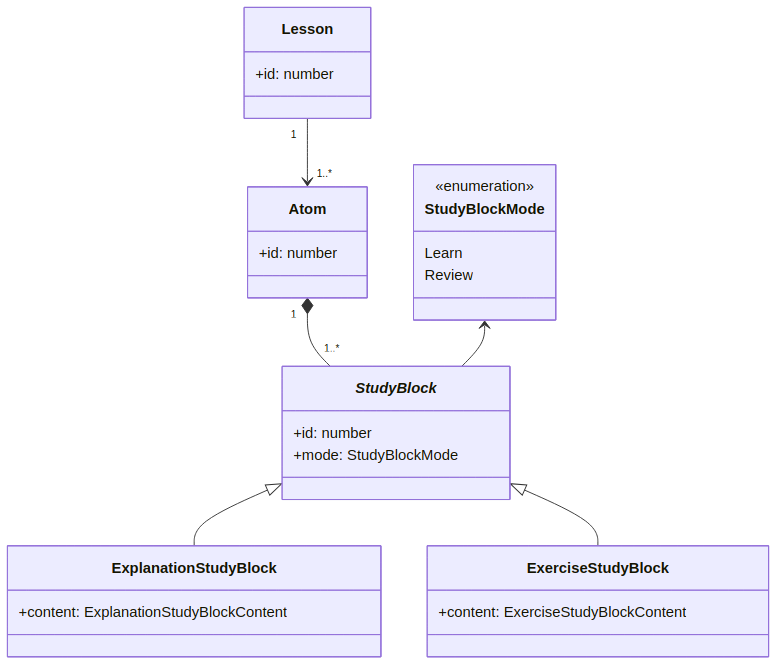
\includegraphics[width=\textwidth]{./images/diagrams/study-model.png}
        \caption{Základní model struktury učení}
        \label{fig:study-model}
    \end{minipage}
\end{figure}

% Final
\subsubsection{Průběh učení a opakování}

% Final
Při spuštění učení je uživateli zobrazena sekvence bloků učení, tedy bloků \texttt{ExplanationStudyBlock} a \texttt{ExerciseStudyBlock}, které jsou v módu \texttt{Learn}. Tento mód indikuje, že mají být bloky použity, pokud je látka pro uživatele nová a dříve se ji neučil. Uživateli je tak pro každý atom v lekci nejprve vysvětlena látka pomocí bloku \texttt{ExplanationStudyBlock}. Následně si uživatel látku procvičí pomocí bloku \texttt{ExerciseStudyBlock}. V rámci každé lekce se tak uživatel postupně naučí několik nových atomů. V průběhu učení aplikace sbírá data o tom, jak uživatel odpovídá v jednotlivých cvičeních. Na základě těchto dat je následně po dokončení lekce naplánováno opakování jednotlivých atomů v backendové části aplikace.

% Final
Pokud uživatel v rámci \texttt{ExerciseStudyBlock} cvičení odpoví špatně, aplikace mu nabídne možnost si zobrazit vysvětlení odpovědi a zkusit cvičení znovu. Pokud uživatel odpoví špatně třikrát po sobě, aplikace mu nabídne možnost daný blok s cvičením přeskočit.

% Final
Při spuštění opakování aplikace uživateli zobrazí pouze sekvence bloků \texttt{ExerciseStudyBlock}, které jsou označeny módem \texttt{Review}. Tyto bloky pomocí cvičení prověří, jak dobře si uživatel danou látku pamatuje. Bloky cvičení jsou vybrány v backendové části aplikace na základě toho, které atomy by si měl uživatel zopakovat podle plánovacího algoritmu. Na základě odpovědí uživatele jsou atomy opět po dokončení učení naplánovány k dalšímu opakování v backendové části aplikace.

% Final
\subsubsection{Vysvětlování látky pomocí \texttt{ExplanationStudyBlock}}

% Final
Vysvětlování látky pomocí \texttt{ExplanationStudyBlock} je tvořeno animacemi doplněnými o audio nahrávku vysvětlující danou látku. Stránky s vysvětlením látky tak připomínají krátká videa, díky kterým je uživateli vysvětlena látka před tím, než začne plnit jednotlivá cvičení. Klíčovým rozdílem oproti klasickým videím je způsob, jakým jsou tato videa vykreslována.

% Final
Na rozdíl od videí, která jsou například uložena ve formátu \texttt{mp4} a následně streamována přes internet, jsou komponenty těchto videí animovány v prohlížeči za běhu aplikace pomocí knihovny Remotion\footnote{Dostupné na: \href{https://www.remotion.dev/}{https://www.remotion.dev/}}. Tyto animace jsou vytvářeny na základě textového popisu videa v JSON formátu, který je obsažený v \texttt{ExplanationStudyBlockContent} v daném \texttt{ExplanationStudyBlock} bloku. Struktura obsahu videí je vyobrazena na diagramu \ref{fig:explanation-model} a budu se ji dále věnovat v následujících částech textu.

% Final
Výše popsaný přístup má několik zásadních výhod a také několik limitací.

% Final
Zaprvé, díky použité knihovně Remotion, která umožňuje snadno animovat UI komponenty za běhu aplikace, je možné snadno vytvořit knihovnu UI komponentů, které mohou být využity při vytváření vysvětlovacích videí. Protože knihovna Remotion pracuje s React komponenty, je možné komponenty videí vytvářet analogickým způsobem, jako zbytek UI komponentů v aplikaci, tedy s využitím zaběhlých jazyků a knihoven. Díky tomu lze v komponentech videí snadno aplikovat existující styly aplikace a zachovat tak naprosto konzistentní vzhled mezi samotnou aplikací a obsahem videí. Pokud bychom se například rozhodli změnit primární barvu nebo jiné styly v aplikaci, bude stejná změna automaticky aplikována ve všech vysvětlovacích videích. Vzhled videí tak bude vždy aktuální a konzistentní se vzhledem celé aplikace.

% Final
Se zmíněnými styly komponentů se pojí i další výhoda, která je spíše vedlejším efektem tohoto přístupu. Protože komponenty videí dodržují stejný styl jako zbytek aplikace, je ve videích reflektován i světlý a tmavý režim aplikace. Byť tento efekt nebyl primárním záměrem použitého přístupu, může výrazně zlepšit uživatelskou zkušenost při sledování videí. Pokud například uživatel preferuje používání aplikace v tmavém režimu při učení se večer, aplikace bude automaticky i všechna videa zobrazovat v tmavém režimu. Učení tak může být pro uživatele výrazně příjemnější.

% Final
Další výhodou je znovupoužitelnost komponentů uživatelského rozhraní. Pokud bychom například vytvořili v aplikaci komponent vizualizující algoritmus Bubble Sort, můžeme tento komponent využít jak v samotných cvičeních, tak ve vysvětlovacích videích. Tato znovupoužitelnost tak může zásadně zefektivnit tvorbu obsahu a zvýšit jeho kvalitu. Při tvorbě obsahu aplikace tak bude možné investovat více času do tvorby a testování jednotlivých komponentů a následně je využívat na více místech napříč cvičeními a videi.

% Final
Další kuriózní výhodou je responzivita samotných videí. Jelikož jsou videa tvořena responzivními UI komponenty, které jsou vykreslovány za běhu aplikace, je možné videa vytvořit tak, aby byly při dodržení určitých rozložení komponentů také responzivní. Videa je tak následně možné sledovat na zařízeních s různě velkými displeji, tedy na počítačích, tabletech i mobilních zařízeních. Docílení této responzivity samozřejmě nebylo přímočaré a bylo třeba zavést řadu opatření, aby byla videa skutečně responzivní. Tomuto tématu se budu podrobněji věnovat v následující podkapitole tohoto textu.

% Final
Kromě výše zmíněných výhod je další zásadní výhodou snadná udržovatelnost a rozšiřitelnost vysvětlovacích videí. Pokud například text ve videu obsahuje chybu nebo nepřesnost, stačí ji opravit v textové definici videa v \texttt{ExplanationStudyBlock} bloku v databázi. Uživatelům se pak začne ihned po načtení učení zobrazovat opravená verze videa. Tyto opravy se netýkají jen obsahu, ale i samotných komponentů videí. Pokud se například některý prvek videa zobrazuje chybně, jeho oprava bude po nasazení frontendu ihned reflektována ve všech vysvětlovacích videích. Tyto snadné změny se netýkají pouze chyb, ale i zdokonalování obsahu a jednotlivých komponentů videí. Díky tomu, že mohou být všechny změny takřka okamžitě aplikovány napříč celou aplikací, je tak možné velice efektivně vytvářet obsah aplikace a vylepšovat jeho kvalitu.

% Final
Poslední výhodou, kterou zde zmíním, je interaktivita samotných videí. Jelikož jsou komponenty videí vykreslovány dynamicky a jedná se o UI komponenty, je možné docílit různých interaktivních efektů. Ve videích je tak možné například vykreslit tlačítko, které bude reagovat na kliknutí uživatele. Jiný komponent může zase například vykreslit aktuální počasí na určitém místě. Byť jsem v rámci této práce do videí žádné interaktivní komponenty nezahrnoval, bude možné v budoucnu videa rozšířit tak, aby byly interaktivnější a poutavější.

% Final
S výše zmíněnými výhodami tohoto přístupu se pojí několik limitací, které je třeba brát v úvahu. Jelikož jsou animace vytvářeny za běhu aplikace v prohlížeči, je třeba brát v potaz výkon prohlížečů, použitých programovacích jazyků a výkon samotných zařízení uživatelů. Prohlížeče s jazykem JavaScript ze své podstaty nebyly vytvořeny primárně pro dynamické vykreslování komplexních videí. Uživatelé mohou také používat aplikaci na různě starých a výkonných zařízeních, což může limitovat schopnost prohlížeče přesně v daném čase animovat jednotlivé komponenty. Kvůli těmto limitacím by bylo nepraktické využívat tento způsob vykreslování pro složitější a graficky náročnější animace. Pokud by například bylo třeba vykreslit vizualizaci nějaké simulace, v níž by se pohybovalo přes deset tisíc prvků, byl by tento přístup takřka nepoužitelný.

% Final
Z výše zmíněného důvodu jsem se rozhodl vytvořit komponent \texttt{Video}, díky kterému je možné do vysvětlovacích videí vložit video ve standardním formátu, tedy například ve formátu \texttt{mp4}. Díky tomu lze kombinovat oba výše zmíněné přístupy. Pro definici struktury videa je tak možné použít přístup popisovaný v této kapitole a pro složitější vizualizace lze na některých místech využít zmíněný komponent \texttt{Video}.

% Final
Další limitací rozebíraného přístupu je responzivita samotných videí. Pokud chceme docílit responzivity videí, je třeba zásadně přizpůsobit rozložení prvků mobilním zařízením, které mají na displeji, ve srovnání s ostatními zařízeními, výrazně méně prostoru. Aby bylo dosaženo plně funkční responzivity, je třeba zásadně zjednodušit strukturu videí a zredukovat tak počet zobrazovaných komponentů, které lze v jednu chvíli ve videu zobrazit. Této responzivitě se budu věnovat v následující podkapitole tohoto textu.

% Final
Poslední limitací, kterou zde zmíním, je použitelnost videí v situacích, kdy uživatel nemá možnost poslouchat audio. Pokud například uživatel jede v autobuse a nemá k dispozici sluchátka, jeho možnost sledovat vysvětlovací videa je značně limitována. Tato limitace vychází spíše z rozhodnutí vysvětlovat látku formou videí, než ze samotného přístupu vykreslování videí. Byť je tato limitace zásadní z hlediska uživatelské zkušenosti, je cenou za získání potenciálně záživnější formy výuky a názornějšího vysvětlování látky.

% Final
Výše zmíněnou limitaci jsem se snažil minimalizovat tím, že jsem k videím implementoval možnost si zobrazit titulky, pokud uživatel nemá možnost poslouchat audio. Uživatelé, kteří nemají možnost poslouchat audio, si tak aspoň mohou při sledování videa číst titulky a získat tak informace touto cestou.

% Final
Celkově tak tato forma vysvětlování látky má několik zásadních výhod a limitací. V rámci této práce jsem došel k názoru, že zmíněné výhody převažují nad nevýhodami a rozhodl jsem se tak v této práci popsaný přístup použít.

% Final
\subsubsection{Responzivita videí s vysvětlením látky}

% Final
V této části textu popíšu, jakým způsobem jsem zajistil responzivitu vysvětlovacích videí, kterou jsem zmínil v předchozí kapitole.

% Final
Aby bylo docíleno responzivního chování videí, bylo třeba, aby videa dodržovala jednoduchou a přesně danou strukturu. Z tohoto důvodu jsem zavedl následující strukturu videí. Každý \texttt{ExplanationStudyBlockContent} se skládá z několika scén \texttt{Scene}. Každá scéna se pak skládá ze stránek \texttt{Slide}, které významově odpovídají stránkám v prezentacích. Každý \texttt{Slide} je pak rozdělen do jednoho až tří sloupců \texttt{Column}, ve kterých jsou následně zobrazovány jednotlivé komponenty. Komponenty ve sloupcích se vždy zobrazují pod sebou v pořadí, ve kterém jsou ve sloupci zadefinovány. 

% Final
Pro zjednodušení tvorby stránek ve videích jsem dále zavedl dva typy stránek. Prvním typem je \texttt{RawSlide}, který umožňuje přesně definovat, které komponenty se mají na stránce zobrazit. Druhým typem je \texttt{SlideTemplate}, který je možné dále rozšiřovat a vytvářet tak předpřipravené šablony stránek. Tyto šablony poskytují oproti \texttt{RawSlide} stránkám zapouzdření jednotlivých komponentů a jednodušší rozhraní. Šablony je tak možné využívat pro efektivnější tvorbu videí. Popsaný model je vyobrazen na diagramu \ref{fig:explanation-model}.

% Review - přizpůsobit textwidth tak, aby se to vešlo do diplomky
\begin{figure}[!h]
    \centering
    \begin{minipage}{0.9\textwidth}
        \centering
        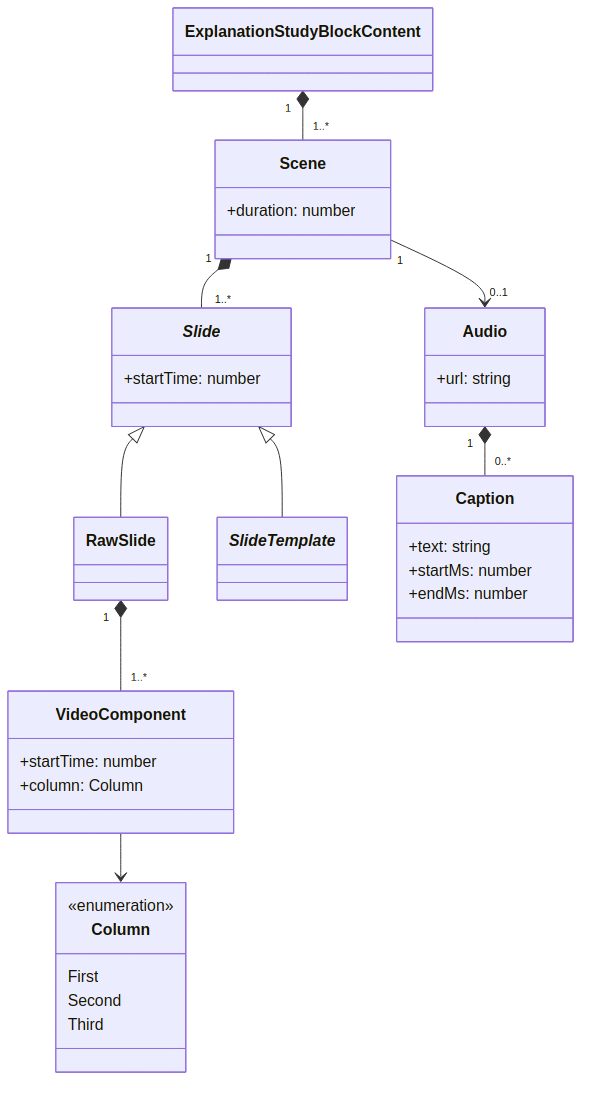
\includegraphics[width=\textwidth]{./images/diagrams/explanation-model.png}
        \caption{Základní model videí s vysvětlením látky}
        \label{fig:explanation-model}
    \end{minipage}
\end{figure}

% Final
Na širokých displejích, tedy například na monitorech nebo mobilních zařízeních orientovaných na šířku, jsou jednotlivé sloupce vykreslovány vedle sebe. Pokud uživatel ovšem sleduje video na zařízení s úzkým displejem, tedy typicky na mobilním zařízení otočeným na výšku, jsou pak sloupce vykreslovány pod sebou. Jednotlivé komponenty se dále přizpůsobují dostupnému místu, podobně jako responzivní komponenty na webových stránkách. Tento systém tak umožňuje snadno umisťovat komponenty na obrazovku tak, aby se jejich rozložení přizpůsobovalo velikosti a orientaci obrazovky.

% Final
Limitací tohoto přístupu je množství komponentů, které je možné ve videu na jedné stránce zobrazit. Do sloupců například není vhodné umisťovat přehršel komponentů s pevně danou výškou, protože by se z důvodu přesunu sloupců na menších displejích pod sebe jednotlivé komponenty nevešly. V důsledku by videa měla být tvořena tak, aby obsahovala více jednodušších stránek s méně komponenty, než méně stránek s mnoha komponenty. Dále, pokud je například třeba zobrazit komplexnější komponent, který obsahuje více detailů nebo textu, je vhodné na obrazovce zobrazit pouze tento komponent v jednom sloupci. Díky tomu bude mít sloupec na všech velikostech displeje maximální výšku a šířku a komponent tak bude možné lépe vidět.

% Final
Samotné komponenty bylo také třeba vytvářet s ohledem na responzivitu videí. Například komponenty zobrazující kód jsem implementoval tak, aby bylo možné při jejich použití určit, v jaké fázi videa se má zobrazit jaká část kódu. Pokud by tak například bylo třeba ve videu ukázat kód s mnoha řádky a vysvětlovat různé části tohoto kódu, je možné v definici komponentu označit jednotlivé části, o kterých se bude ve videu ve vybraném čase mluvit. Aplikace pak bude automaticky v daném čase scrollovat na specifikovanou část kódu, díky čemuž bude moci uživatel vždy na obrazovce vidět, o které části kódu je ve videu řeč.

% Final
\subsubsection{Plnění cvičení pomocí \texttt{ExerciseStudyBlock}}

% Final
Po tom, co byla v rámci učení uživateli vysvětlena látka pomocí dříve popsaných bloků s vysvětlením látky \texttt{ExplanationStudyBlock}, jsou uživateli zobrazeny bloky \texttt{ExerciseStudyBlock}, které slouží k procvičení dané látky a sběru dat o tom, jak uživatel dané látce rozumí.

% Final
Každý tento blok je, podobně jako bloky s vysvětlením látky, vykreslen na samostatné stránce v rámci učení. Tento blok může obsahovat jeden nebo více komponentů \texttt{ExerciseStudyBlockComponent}, které jsou vykresleny pod sebou v jednom sloupci. Komponenty jsou buď pasivní, které pouze zobrazují informace, nebo aktivní, se kterými může uživatel interagovat. Pasivní komponenty jsou například nadpisy, odstavce nebo diagramy. Aktivními komponenty jsou různá cvičení, které musí uživatel vyplnit pro splnění daného bloku. Jeden \texttt{ExerciseStudyBlock} může obsahovat více aktivních komponentů. Příkladem toho je editor kódu, který obsahuje více oken s kódem. Každé okno je pak považováno za samostatný komponent cvičení.

% Final
Po vyplnění všech aktivních komponentů v rámci daného bloku uživatel zvolí možnost zkontrolovat výsledky, aplikace odpověď ohodnotí a zaznamená. Uživatel má pak možnost pokračovat nebo odpověď opravit v případě, že byla špatná.

% Final
Podobně jako bloky s vysvětlením látky, mohou bloky se cvičeními obsahovat audio nahrávku, která doprovází uživatele při učení. Na rozdíl od bloků s vysvětlením látky, kde je audio nahrávka přehrávána v rámci celého videa, je v případě bloků se cvičeními audio nahrávka pouze připojena ke konkrétním komponentům. Každý komponent tak k sobě může mít připojenou audio nahrávku, která například vysvětluje zadání daného příkladu. Po načtení \texttt{ExerciseStudyBlock} bloku se postupně přehrají všechny audio nahrávky, které jsou v komponentech daného bloku obsaženy. Díky tomu například uživatel nemusí číst text se zadáním, ale může si ho poslechnout a následně hned vyplnit dané cvičení.

% Final
Díky audio nahrávkám a flexibilní struktuře bloků cvičení a vysvětlování látky je tak možné pro uživatele vytvářet vysoce interaktivní průchody učením a opakováním. Způsob výuky v této aplikaci se tak blíží interaktivním lekcím konkurenčních aplikací Scrimba a Mimo, které jsem analyzoval v rámci analýzy existujících řešení.

% Write - tuhle sekci sepsat
\subsection{Push Notifikace}

% Review
\subsection{Přizpůsobení aplikace pro PWA}

% Review
V rámci nefunkčního požadavku jsem doplnil konfiguraci aplikace nutnou pro to, aby prohlížeče aplikaci klasifikovaly jako progresivní webovou aplikaci. V souboru \texttt{manifest.ts} jsem definoval metadata aplikace, jako například název, jazyk aplikace, základní barvy a ikony. V rámci této konfigurace jsem také vytvořil několik základních ikon, které může progresivní webová aplikace využívat.

% Review
Dále jsem do aplikace doplnil registraci tzv. Service Worker služby. Service Worker je skript běžící v prohlížeči, jehož životní cyklus je takřka nezávislý na životním cyklu aplikace. Service Worker tak může běžet ve vlastním vlákně nezávisle na samotné aplikaci. Tato služba se využívá například pro správu cache aplikace, podporu offline funkcí a jako proxy mezi odchozími a příchozími požadavky a samotnou aplikací. V rámci této práce jsem se těmto funkcím nevěnoval a proto jsem pouze zaregistroval prázdný Service Worker skript, který je nutný pro vytvoření PWA. \cite{ServiceWorker}

% Review
Nakonec bylo třeba zajistit, aby byla aplikace dostupná přes HTTPS protokol \cite{PWABuilder}. To jsem zajistil v rámci nasazení aplikace, kterému se věnuji v podkapitole \nameref{sec:deployment}.

% Review
Díky výše zmíněné konfiguraci se tak aplikace stala progresivní webovou aplikací. Uživatelé si tak mohou aplikaci stáhnout a nainstalovat do svých zařízení přímo z prohlížeče na stránkách této aplikace.

% Review
Aplikaci tak bude možné v budoucnu po dalších konfiguracích, například s pomocí nástroje PWABuilder \cite{PWABuilder}, zabalit a publikovat na platformách Google Play, App Store nebo například Microsoft Store. Publikace na tyto platformy je časově značně náročná a týká se spíše právních otázek, nežli softwarového inženýrství. Proto se samotné publikaci v rámci této práce nebudu věnovat.

% Final
\section{Nasazení aplikace}\label{sec:deployment}

% Final
V rámci nasazování aplikace jsem vytvořil tři samostatná prostředí aplikace \texttt{dev}, \texttt{stage} a \texttt{production}. Každé prostředí má odlišný účel, odlišné napojení na API a odlišný způsob nasazení. Kromě nasazení aplikace bylo třeba také zajistit, aby byly k dispozici pro stažení a instalaci vytvořené knihovny \texttt{@eduriam/ui-core} a \texttt{@eduriam/ui-x}. Těmto tématům se budu věnovat v této podkapitole.

% Final
\subsection{Testovací prostředí \texttt{dev}}

% Final
Testovací prostředí \texttt{dev} je dostupné na adrese \texttt{dev.eduriam.com}. Hosting je zajištěn na platformě Vercel. Tento hosting jsem zvolil jednak protože původní aplikace tento hosting využívala a jednak protože společnost Vercel vyvíjí framework Next.js, ve kterém je tato aplikace naprogramována. Aplikace v tomto prostředí využívá mock backendového API, který je nasazený na platformě Netlify.

% Final
Nasazení do tohoto prostředí probíhá automaticky při každém provedení příkazu \texttt{git push} do větve \texttt{dev} v repozitáři frontendu aplikace. Při provedení této akce se provede jak nasazení aplikace, tak nasazení zmíněného mocku API.

% Final
Toto prostředí slouží k několika účelům. Jednak slouží k rychlému vyvíjení a testování funkcí aplikace, které ještě nejsou podporovány backend API. Dále lze toto prostředí snadno využít například pro uživatelské testování a validaci nových funkcí. Toto prostředí jsem také vytvořil z důvodu, že bylo podobné prostředí využíváno v původní aplikaci. Vzhledem k vytvoření nového testovacího prostředí \texttt{stage} bude v budoucnu stát za úvahu odstranění prostředí \texttt{dev}, pokud již nebude využíváno.

% Final
\subsection{Testovací prostředí \texttt{stage}}

% Final
Testovací prostředí \texttt{stage} je dostupné na adrese \texttt{app.stage.eduriam.com} a rovněž využívá hosting společnosti Vercel. Na rozdíl od prostředí \texttt{dev} je toto prostředí napojeno na stage verzi backendového API, tedy na reálnou implementaci API určenou pro testování.

% Final
Nasazení frontendu do \texttt{stage} probíhá také automaticky při každém provedení \texttt{git push} do větve \texttt{dev}. Nasazením backendu se zabývá kolega Bc. Jakub Vondráček v jeho diplomové práci.

% Final
Stage prostředí představuje hlavní testovací prostředí, ve kterém lze ověřovat chování aplikace se skutečnými koncovými body API. Toto prostředí lze využít pro uživatelské testování nebo manuální testování jednotlivých funkcí.

% Final
\subsection{Produkční prostředí \texttt{production}}

% Final
Produkční prostředí \texttt{production} je dostupné na adrese \texttt{app.eduriam.com} a je napojeno na produkční backendové API. Podobně jako ostatní prostředí je toto prostředí nasazeno na platformě společnosti Vercel.

% Final
Nasazení probíhá při manuálním vytvoření release značky na git větvi \texttt{master}, což odpovídá procesu nasazování, který byl zaveden v původní aplikaci. Nasazením produkčního API se opět zabývá kolega Bc. Jakub Vondráček v jeho diplomové práci.

% Final
Produkční prostředí představuje hlavní prostředí, ve kterém je aplikace veřejně dostupná uživatelům.

% Final
\subsection{Nasazení knihoven komponentů}

% Final
Kromě nasazení frontendu bylo třeba zajistit, aby byly k dispozici pro stažení a instalaci nově vytvořené knihovny \texttt{@eduriam/ui-core} a \texttt{@eduriam/ui-x}. Knihovny jsem se rozhodl hostovat na platformě GitHub s využitím služby GitHub Packages\footnote{Dostupné na: \href{https://docs.github.com/packages}{https://docs.github.com/packages}}. Tato platforma umožňuje snadno hostovat a distribuovat knihovny sestavením balíčků přímo z GitHub repozitáře.

% Final
Nasazení nové verze probíhá automaticky při provedení příkazu \texttt{git merge} z větve \texttt{dev} do větve \texttt{main} v repozitáři knihoven, pokud byla v rámci změn navýšena verze některé knihovny v souboru \texttt{package.json}. Po nasazení lze knihovny stáhnout a instalovat pomocí nástrojů \texttt{npm} nebo \texttt{yarn} podobně jako ostatní knihovny.


% Chapter: Testing
% Final
\chapter{Testování}

% Final
V této kapitole se budu zabývat testováním aplikace, které je klíčovou součástí vývoje a pomáhá zajistit kvalitu a stabilitu jednotlivých funkcí. Nejprve se zaměřím na volbu vhodných forem testování s ohledem na rozsah a zaměření tohoto projektu. Dále popíšu, jakým způsobem jsem prováděl manuální testování, automatizované end-to-end testování a uživatelské testování. Na závěr zhodnotím celou aplikaci a navrhnu možnosti jejího dalšího rozvoje do budoucna.

% Done
\section{Volba vhodných forem testování}

% Review
V této sekci se budu věnovat volbě vhodných forem testování. Forem testování existuje celá řada a každá forma testování je vhodná pro různé účely a projekty. Při volbě testování jsem zvažoval různé formy testování, včetně manuálního testování, automatizovaných testů a testů použitelnosti.

% Review
Jako první formu testování jsem zvolil manuální testování, které mi umožnilo v průběhu vývoje aplikace cíleně testovat části, které jsem implementoval. Způsob využití tohoto testování podrobněji popíšu v dalších částech tohoto textu.

% Review
Dále jsem se v rámci volby vhodných forem testování rozhodl zavést do aplikace automatizované testy. Automatizované testy umožní v aplikaci stanovit určitý standard kvality a stability funkcí, což je klíčové pro dlouhodobé fungování aplikace. Automatizované testy jsem se také rozhodl do aplikace zavést v souladu s návrhem úprav do budoucna původní aplikace, který jsem popsal v rámci mé bakalářské práce \cite{Jenicek2024BachelorThesis}. 

% Review
V rámci automatizovaných testů jsem se rozhodl zavést do aplikace automatizované end-to-end testy. Tyto testy umožní testovat funkčnost aplikace jako celku a ověřit tak, že se aplikace skutečně chová dle očekávání a specifikovaných požadavků. Tento typ automatizovaných testů jsem zvolil zejména kvůli tomu, že frontendová část aplikace cíleně neobsahuje velké množství byznys logiky a její komponenty jsou cíleně navrženy co nejjednodušším způsobem. End-to-end testy jsem tak vyhodnotil jako nejlepší přístup, protože v kombinaci se zvolenou metodikou BDD a nástrojem Cucumber popsanými v kapitole \nameref{sec:gherkin-specification} umožňují velice efektivně ověřit základní funkčnost všech implementovaných funkcí. S ohledem na přínos těchto testů a jejich efektivitu implementace jsem tak vyhodnotil, že tyto testy přinesou nejvyšší přínos v poměru k množství investovaného času a zdrojů.

% Review
V rámci zajištění kvality celé aplikace jsem se dále rozhodl provést testy použitelnosti. Konkrétně jsem se rozhodl provést kvalitativní uživatelské testování, které umožní ověřit, že jsou implementované funkce snadno a srozumitelně použitelné z pohledu uživatele \cite{NURUserInterfaceTesting}. Tomuto testování se opět budu podrobněji věnovat v následujících částech tohoto textu.

% Review
Kombinací zvolených testů tak vznikne ucelený systém testování, díky kterému bude možné zajistit vyšší kvalitu a stabilitu celé aplikace. Automatizované end-to-end testy zajistí základní funkčnost všech implementovaných funkcí a dále zajistí, že kriticky důležité funkce aplikace stále fungují před nasazením aplikace do produkčního prostředí. Manuální testování pak umožňuje se efektivně zaměřit na specifické problémy a chyby v aplikaci. Kvalitativní uživatelské testování dále umožní zajistit, že aplikace skutečně pokrývá potřeby uživatelů a že jsou funkce pro uživatele srozumitelné a snadno použitelné.

% Done
\section{Manuální testování}

% Write
Prvním prováděným testováním bylo manuální testování. Toto testování mi umožnilo v průběhu vývoje cíleně testovat funkce, které jsem implementoval.
% Done
\section{End-to-end testování s mock API}

% Done
\section{Uživatelské testování}

% Done
\subsection{Plán testování}

% Done
\subsection{Testovací scénáře}

% Done
\subsection{Průběh testování}

% Done
\subsection{Výsledky testování}
% Done
\section{Zhodnocení řešení a návrh úprav do budoucna}

% Done
\subsection{Zhodnocení řešení}

% Done
\subsection{Návrh úprav do budoucna}

% Chapter: Conclusion
% Review
\chapter*{Závěr}\addcontentsline{toc}{chapter}{Závěr}\markboth{Závěr}{Závěr}

% Review
Cílem této práce bylo ve spolupráci s Bc. Jakubem Vondráčkem realizovat vzdělávací webovou aplikaci určenou pro samouky, kteří se chtějí naučit základy programování. Práce vycházela z již existující aplikace pro výuku anglického jazyka, kterou bylo nutné upravit a rozšířit pro potřeby výuky programování. Z důvodu rozsahu celého řešení se tato práce zaměřovala na frontendovou část aplikace, zatímco backendová část byla předmětem diplomové práce kolegy.

% Review
V rámci analýzy jsem porovnal vybraná konkurenční řešení, analyzoval původní aplikaci pro výuku angličtiny a definoval funkční a nefunkční požadavky se zaměřením na frontendovou část aplikace. Na základě těchto požadavků jsem následně navrhl nové funkce a úpravy existujících funkcí. V rámci této fáze jsem dále vytvořil návrh uživatelského rozhraní aplikace.

% Review
Ve fázi implementace jsem upravil frontend původní aplikace podle navrženého řešení. Odstranil jsem funkce, které nebyly pro novou aplikaci relevantní a implementoval jsem všechny definované požadavky. Frontend aplikace jsem dále nasadil do testovacího a produkčního prostředí.

% Review
Do aplikace jsem zavedl zjednodušené automatizované end-to-end testy, které ověřují funkčnost frontendové části aplikace s využitím mock API. Při vývoji aplikace jsem také prováděl manuální testování jednotlivých komponentů a stránek aplikace. Dále jsem provedl kvalitativní uživatelské testování zaměřené na použitelnost aplikace. Problémy, které byly při testování zjištěny, jsem následně opravil. Nakonec jsem zhodnotil výsledné řešení a navrhl možnosti rozvoje aplikace do budoucna.

% Review
Celkově tak bylo dosaženo všech stanovených cílů této práce. Výsledkem je nasazená frontendová část aplikace, která společně s backendovou částí tvoří funkční vzdělávací aplikaci. Díky této aplikaci se tak budou moci uživatelé naučit základy programování a aplikace je připravena pro další rozvoj.


\appendix\appendixinit % do not remove these two commands

% Chapter: Test results
\addtocontents{toc}{\protect\setcounter{tocdepth}{0}}
\include{text/appendix/requirements-list}
% Final
\chapter{Seznam nefunkčních požadavků}\label{chapter:non-functional-requirements-list}

% Final
V této příloze lze nalézt seznam všech nefunkčních požadavků aplikace.


% Final
\section*{NP-1 Odstranění přebytečných funkcí}\label{sec:np-remove-extra-functions}

% Final
\begin{tabular}{lp{0.7\linewidth}}
    \textbf{Priorita:} & Must have \\
    \textbf{Kategorie:} & Udržovatelnost systému \\
\end{tabular}

% Final
Jelikož se nově vznikající aplikace bude zaměřovat na výuku programování, bude třeba odstranit funkce týkající se původní domény výuky jazyků. Tyto funkce jsem specifikoval v rámci analýzy stávajícího řešení.

% Final
\section*{NP-2 Nový design uživatelského rozhraní}\label{sec:np-new-ui-design}

% Final
\begin{tabular}{lp{0.7\linewidth}}
    \textbf{Priorita:} & Must have \\
    \textbf{Kategorie:} & Použitelnost systému \\
\end{tabular}

% Final
Jelikož aplikace mění své zaměření z výuky jazyků na výuku programování, je třeba kompletně změnit a přizpůsobit i celý vzhled uživatelského rozhraní. Měl by tak být vytvořen kompletně nový návrh uživatelského rozhraní, který se bude zahrnovat jak nové, tak i existující funkce aplikace.

% Final
\section*{NP-3 Zpřehlednění navigace v aplikaci}\label{sec:np-navigation-clarity}

% Final
\begin{tabular}{lp{0.7\linewidth}}
    \textbf{Priorita:} & Should have \\
    \textbf{Kategorie:} & Použitelnost systému \\
\end{tabular}

% Final
Aplikace by měla uživateli poskytovat přehlednější a jednodušší způsob navigace mezi jednotlivými stránkami. Z výsledků uživatelského testování v mé bakalářské práci \cite{Jenicek2024BachelorThesis}, která se zabývala původní aplikací, vyplynulo, že mají uživatelé problém s navigací mezi jednotlivými stránkami aplikace, zejména mezi jednotlivými sekcemi kurzů. Jelikož bude do aplikace také přidána řada nových funkcí, bude třeba navigaci aktualizovat tak, aby se uživatel mohl snadno orientovat v aplikaci a využívat všechny dostupné funkce.

% Final
\section*{NP-4 Vytvoření knihovny komponentů}\label{sec:np-component-library}

% Final
\begin{tabular}{lp{0.7\linewidth}}
    \textbf{Priorita:} & Should have \\
    \textbf{Kategorie:} & Rozšiřitelnost systému \\
\end{tabular}

% Final
Frontend aplikace využívá různé komponenty uživatelského rozhraní. Tyto komponenty by měly být přesunuty do samostatné knihovny tak, aby je bylo možné využít i v dalších částech projektu, jako například na webových stránkách nebo v systému pro správu obsahu aplikace.

% Final
Tato knihovna komponentů by měla stavět na již existujících komponentech a měla by využívat již zavedené technologie, tedy jazyk TypeScript a knihovny React, Storybook a Material UI.

% Final
\section*{NP-5 Zvýšení udržovatelnosti kódu}\label{sec:np-maintainability}

% Final
\begin{tabular}{lp{0.7\linewidth}}
    \textbf{Priorita:} & Should have \\
    \textbf{Kategorie:} & Udržovatelnost systému \\
\end{tabular}

% Final
Na základě analýzy stávající aplikace jsem se rozhodl přizpůsobit kód aplikace tak, aby byl lépe udržovatelný a rozšiřitelný. Konkrétní změny, které bude třeba provést, jsem popsal v rámci analýzy stávajícího řešení.

% Final
\section*{NP-6 Zavedení automatizovaných testů}\label{sec:np-automated-tests}

% Final
\begin{tabular}{lp{0.7\linewidth}}
    \textbf{Priorita:} & Should have \\
    \textbf{Kategorie:} & Použitelnost systému \\
\end{tabular}

% Final
Do frontendové části aplikace by měly být zavedeny automatizované testy s cílem zajištění správného fungování aplikace a zvýšení její kvality a použitelnosti.

% Final
Tento požadavek vychází jednak z analýzy existujícího řešení a jednak z návrhu úprav do budoucna, který jsem popsal v rámci mé bakalářské práce \cite{Jenicek2024BachelorThesis}, která se věnovala původní aplikaci.

% Final
\section*{NP-7 Automaticky generované třídy API}\label{sec:np-generated-api-classes}

% Final
\begin{tabular}{lp{0.7\linewidth}}
    \textbf{Priorita:} & Should have \\
    \textbf{Kategorie:} & Udržovatelnost systému \\
\end{tabular}

% Final
V kódu frontendové části aplikace by měly být automaticky generovány třídy reprezentující backendové API na základě OpenAPI specifikace \cite{OpenAPISpecification}, která je poskytována backendovou částí aplikace.

% Final
Požadavek vychází z analýzy existujícího řešení. Cílem tohoto požadavku je zjednodušit implementaci a zajistit konzistenci mezi frontendovou a backendovou částí aplikace.

% Final
\section*{NP-8 Animace a efekty}\label{sec:np-animations-effects}

% Final
\begin{tabular}{lp{0.7\linewidth}}
    \textbf{Priorita:} & Could have \\
    \textbf{Kategorie:} & Použitelnost systému \\
\end{tabular}

% Final
Do aplikace by měly být přidány základní animace a efekty s cílem zlepšit uživatelskou zkušenost a udržet pozornost uživatelů. Uživatelské rozhraní by tak mělo působit vizuálně poutavějším dojmem a mělo by výrazněji reagovat na interakce s uživatelem.

% Final
Tento požadavek vychází zejména z analýzy konkurenčních řešení, ve které konkurenční aplikace Mimo nebo Scrimba využívají různé animace a efekty.

% Final
\section*{NP-9 Nasazení aplikace jako PWA}\label{sec:np-pwa-deployment}

% Final
\begin{tabular}{lp{0.7\linewidth}}
    \textbf{Priorita:} & Should have \\
    \textbf{Kategorie:} & Použitelnost systému \\
\end{tabular}

% Final
Aplikace by měla být přizpůsobena tak, aby bylo možné ji sestavit a nasadit jako PWA, neboli jako progresivní webovou aplikaci. V důsledku toho by mělo být možné aplikaci stáhnout a nainstalovat na zařízení s operačními systémy Windows, Android či iOS. K aplikaci by tak mělo být možné přistupovat buď na webových stránkách, nebo přímo na zařízení uživatele.

\include{text/appendix/use-case-list}
% Final
\chapter{Zadání uživatelského testování}\label{chapter:test-scenarios}

% Final
V této příloze lze nalézt zadání uživatelského testování použitelnosti aplikace.

% Final
\section{TS1 -- Registrace a zapsání kurzu}

% Final
\paragraph{Zadání} Otevřel jste aplikaci na učení se programování. Založte si v aplikaci účet, vyplňte úvodní dotazník a zapište si kurz \textit{HTML}. Při registraci použijte uživatelské jméno \textit{Test}, e-mail \textit{test@example.com} a heslo \textit{Test1234}.

% Final
\paragraph{Očekávaný průchod aplikací}

% Final
\begin{enumerate}
    \item Uživatel začíná na úvodní stránce aplikace.
    \item Uživatel se z úvodní stránky přesune na stránku registrace, vyplní registrační formulář a zvolí možnost zaregistrovat se. Aplikace přesune uživatele na stránku úvodního dotazníku.
    \item V dotazníku uživatel vyplní svoji úroveň programování, témata, která se chce učit, a cíl, kterého chce dosáhnout.
    \item Následně uživatel vybere jeden z doporučených kurzů.
    \item Nakonec uživatel zvolí svůj denní cíl učení.
    \item Aplikace oznámí uživateli, že je jeho účet připraven a uživatel zvolí možnost pokračovat, čímž se přesune na hlavní stránku aplikace.
\end{enumerate}

% Final
\section{TS2 -- Učení se dle studijního plánu}

% Final
\paragraph{Zadání} Otevřel jste aplikaci a chcete se začít učit vámi zapsaný kurz. Spusťte nadcházející lekci kurzu a lekci dokončete.

% Final
\paragraph{Očekávaný průchod aplikací}

% Final
\begin{enumerate}
    \item Uživatel začíná na hlavní stránce aplikace.
    \item Uživatel zvolí možnost spustit nadcházející lekci kurzu.
    \item Aplikace přesune uživatele na stránku učení, kde mu zobrazí látku nadcházející lekce.
    \item Uživatel splní všechna cvičení v lekci a aplikace mu oznámí, že byla lekce dokončena.
    \item Uživatel zvolí možnost pokračovat a aplikace ho přesměruje zpět na hlavní stránku.
\end{enumerate}

% Final
\section{TS3 -- Zapsání nového kurzu}

% Final
\paragraph{Zadání} Chcete si zapsat nový kurz \textit{CSS}. Zapište si tento kurz a spusťte v něm první lekci. Tuto lekci dokončete.

% Final
\paragraph{Očekávaný průchod aplikací}

% Final
\begin{enumerate}
    \item Uživatel začíná na hlavní stránce aplikace.
    \item Uživatel zvolí ikonu studijního plánu, čímž se přesune na stránku studijního plánu.
    \item Na stránce studijního plánu uživatel zvolí možnost přidat nový kurz, čímž se přesune na stránku s výběrem kurzů.
    \item Na stránce výběru kurzů uživatel zvolí kurz \textit{CSS}, čímž se přesune na stránku kurzu.
    \item Na stránce kurzu pak uživatel zvolí možnost začít kurz, čímž mu bude kurz zapsán a uživatel bude přesměrován na stránku učení první lekce kurzu.
    \item Uživatel splní všechna cvičení v lekci a aplikace mu oznámí, že byla lekce dokončena.
    \item Uživatel zvolí možnost pokračovat a aplikace ho přesměruje zpět na hlavní stránku.
\end{enumerate}

% Final
\section{TS4 -- Úprava studijního plánu}

% Final
\paragraph{Zadání} Máte zapsané kurzy \textit{HTML} a \textit{CSS}, které jste se nějakou dobu učili. Nyní se chcete zaměřit pouze na kurz CSS a z kurzu HTML se již nechcete učit nové lekce. Zařiďte, aby vám aplikace na hlavní stránce již nezobrazovala nové lekce z kurzu HTML, ale abyste nepřišli o svůj pokrok v kurzu HTML.

% Final
\paragraph{Očekávaný průchod aplikací}

% Final
\begin{enumerate}
    \item Uživatel začíná na hlavní stránce aplikace.
    \item Uživatel zvolí ikonu studijního plánu, čímž se přesune na stránku studijního plánu.
    \item Na stránce studijního plánu uživatel přesune kurz \textit{HTML} ze sekce Učení a opakování do sekce Pozastaveno. Aplikace mu tak na hlavní stránce přestane zobrazovat nové lekce z kurzu HTML.
\end{enumerate}

% Final
\section{TS5 -- Spuštění konkrétní lekce}

% Final
\paragraph{Zadání} V rámci kurzu HTML se chcete naučit látku z lekce \textit{Obrázky}. Spusťte tuto konkrétní lekci a dokončete ji.

% Final
\paragraph{Očekávaný průchod aplikací}

% Final
\begin{enumerate}
    \item Uživatel začíná na hlavní stránce aplikace.
    \item Uživatel zvolí ikonu studijního plánu, čímž se přesune na stránku studijního plánu.
    \item Na stránce studijního plánu uživatel zvolí kurz \textit{HTML}, čímž se přesune na stránku kurzu.
    \item Na stránce kurzu uživatel vybere první kapitolu kurzu, čímž se přesune na stránku dané kapitoly.
    \item Na stránce kapitoly kurzu uživatel najde lekci \textit{Obrázky} a zvolí možnost spuštění lekce.
    \item Uživatel splní všechna cvičení v lekci a aplikace mu oznámí, že byla lekce dokončena.
    \item Uživatel zvolí možnost pokračovat a aplikace ho přesměruje zpět na hlavní stránku.
\end{enumerate}

% Final
\section{TS6 -- Zakoupení položky a změna vzhledu avatara}

% Final
\paragraph{Zadání} Za učení jste získali virtuální měnu. Kupte si položku v obchodě a zajistěte, aby se tato položka zobrazovala na vašem profilovém obrázku.

% Final
\paragraph{Očekávaný průchod aplikací}

% Final
\begin{enumerate}
    \item Uživatel začíná na hlavní stránce aplikace.
    \item Uživatel zvolí ikonu profilu, čímž se přesune na stránku profilu.
    \item Na stránce profilu dále zvolí ikonu obchodu, čímž se přesune na stránku obchodu.
    \item Na stránce obchodu uživatel zvolí libovolnou položku a zvolí možnost koupit položku.
    \item Poté se uživatel kliknutím na tlačítko zpět přesune na stránku profilu.
    \item Na stránce profilu uživatel klikne na svého avatara, čímž se přesune na stránku přizpůsobení avatara.
    \item Na stránce přizpůsobení avatara zvolí zakoupenou položku, kterou chce přidat na svůj profilový obrázek a změnu uloží.
    \item Aplikace uživatele přesune na stránku profilu.
\end{enumerate}
% Final
\chapter{Výsledky uživatelského testování}\label{chapter:test-problems}

% Final
V této příloze shrnu výsledky uživatelského testování, konkrétně problémy, nedostatky a návrhy na zlepšení testované aplikace. U každého problému jsem určil jeho závažnost a navrhl jeho možné řešení.

% Final
\section*{Problém 1 – Není možné zobrazit heslo při registraci}

% Final
\begin{tabular}{lp{0.7\linewidth}}
    \textbf{Popis:} & Při vyplňování formuláře pro registraci aplikace neumožňuje uživateli si zobrazit vyplňované heslo. Většina uživatelů při testování zmínila, že jim tato možnost v aplikaci chybí. Podobný problém nastává i při přihlašování a změně existujícího hesla.\\
    \textbf{Možné řešení:} & Přidat do textového pole hesla tlačítko s ikonou oka umožňující zobrazit zadávané heslo. \\
    \textbf{Závažnost:} & Střední \\
    % Final
    \textbf{Stav:} & Opraveno  \\
\end{tabular}

% Final
\section*{Problém 2 – Není zřejmé, ze kterého kurzu je vybrána lekce dle studijního plánu}

% Final
\begin{tabular}{lp{0.7\linewidth}}
    \textbf{Popis:} & Na hlavní stránce není uživatelům jasné, ze kterého kurzu je vybrána nadcházející lekce podle studijního plánu. Uživatelé tak neví, který kurz se momentálně učí. \\
    \textbf{Možné řešení:} & Přidat na hlavní stránku informaci o tom, ze kterého kurzu je daná lekce vybrána. \\
    \textbf{Závažnost:} & Vysoká \\
    % Final
    \textbf{Stav:} & Opraveno  \\
\end{tabular}

% Final
\section*{Problém 3 – Upoutávka na lekci je pro uživatele matoucí}

% Final
\begin{tabular}{lp{0.7\linewidth}}
    \textbf{Popis:} & Na hlavní stránce se zobrazuje upoutávka na nadcházející lekci ve formátu GIF ukazující průběh vybrané lekce. Cílem tohoto návrhu bylo pomocí ukázky upoutat pozornost uživatele a přimět ho si lekci spustit. Uživatelské testování ovšem ukázalo, že je tato upoutávka z důvodu struktury lekcí příliš nevýrazná a není tak pro uživatele vizuálně poutavá. Pro většinu uživatelů byla naopak tato upoutávka matoucí.  \\
    \textbf{Možné řešení:} & Nahradit GIF upoutávku statickým obrázkem či logem, který bude reprezentovat danou lekci. \\
    \textbf{Závažnost:} & Vysoká \\
    % Final
    \textbf{Stav:} & Opraveno  \\
\end{tabular}

% Final
\section*{Problém 4 – Zvýrazňování tlačítek při jejich stisknutí na mobilních zařízeních}

% Final
\begin{tabular}{lp{0.7\linewidth}}
    \textbf{Popis:} & Jeden z uživatelů vhodně poznamenal, že při kliknutí na libovolné tlačítko se na mobilních zařízeních na krátkou chvíli zobrazí modrý rámeček kolem daného tlačítka. Tento nežádoucí efekt pak má za důsledek to, že z pohledu uživatele aplikace vypadá nefunkčně, obzvláště pokud se rámeček zobrazuje u tlačítek jiných tvarů, jako například u kulatého profilového obrázku uživatele.  \\
    \textbf{Možné řešení:} & Zadefinovat styly aplikace, které budou tomuto výchozímu chování předcházet. \\
    \textbf{Závažnost:} & Střední \\
    % Final
    \textbf{Stav:} & Opraveno  \\
\end{tabular}

% Final
\section*{Problém 5 – Pomocná nabídka znaků překrývá tlačítko pro pokračování lekce}

% Final
\begin{tabular}{lp{0.7\linewidth}}
    \textbf{Popis:} & Při vyplňování cvičení, ve kterých má uživatel za úkol ručně doplňovat kód, je uživateli na mobilních zařízeních zobrazena pomocná nabídka znaků, díky které má jednodušší přístup k některým znakům. Díky této nabídce může snadno doplňovat do kódu speciální znaky a následně potvrdit svoji odpověď. Testování ovšem ukázalo, že tato nabídka překrývá původní tlačítko pro kontrolu odpovědi v jednotlivých cvičeních a pro uživatele tak může být obtížné svoji odpověď potvrdit. \\
    \textbf{Možné řešení:} & Změnit zobrazování pomocné nabídky tak, aby se zobrazila pouze, pokud má uživatel vybrané některé z textových polí. \\
    \textbf{Závažnost:} & Vysoká \\
    % Final
    \textbf{Stav:} & Opraveno  \\
\end{tabular}

% Final
\section*{Problém 6 – Možnost přetahování slov z nabídky slov při vyplňování cvičení}

% Final
\begin{tabular}{lp{0.7\linewidth}}
    \textbf{Popis:} & V aplikaci existuje cvičení, ve kterém mají uživatelé za úkol doplnit kód pomocí slov z nabídky. Momentální implementace umožňuje doplňování pouze pomocí klikání na jednotlivá slova v nabídce. Přestože všichni uživatelé zvládli tímto způsobem cvičení vyplnit, ukázalo se, že část uživatelů má tendenci toto cvičení vyplňovat přetahováním jednotlivých slov z nabídky na daná místa v kódu. Toto přetahování ovšem není v aplikaci implementováno. \\
    \textbf{Možné řešení:} & Zavést do aplikace možnost vyplňovat slova z nabídky pomocí přetahování jednotlivých slov. \\
    \textbf{Závažnost:} & Střední \\
    % Final
    \textbf{Stav:} & Opraveno  \\
\end{tabular}

% Final
\section*{Problém 7 – Persistence nastavení hlasu napříč lekcemi}

% Final
\begin{tabular}{lp{0.7\linewidth}}
    \textbf{Popis:} & V rámci učení mohou být cvičení doplněna o audionahrávky vysvětlující zadání daného cvičení. Někteří uživatelé ovšem vyjádřili preferenci cvičení vyplňovat bez zvuku a označili zvuk za rušivý. Aplikace již umožňuje vypnout zvuk cvičení v rámci dané lekce, nicméně toto nastavení není zachováno napříč jednotlivými lekcemi. Z důvodu silné preference některých uživatelů by bylo vhodné toto nastavení zachovat napříč lekcemi, aby uživatelé nebyli nuceni zvuk neustále vypínat. \\
    \textbf{Možné řešení:} & Uložit nastavení zvuku tak, aby bylo zachováno napříč lekcemi. \\
    \textbf{Závažnost:} & Vysoká \\
    % Final
    \textbf{Stav:} & Opraveno  \\
\end{tabular}

% Final
\section*{Problém 8 – Zobrazování výstupu kódu při učení}

% Final
\begin{tabular}{lp{0.7\linewidth}}
    \textbf{Popis:} & V rámci učení mají uživatelé možnost si zobrazit výstup kódu například v podobě terminálu nebo webové stránky. Momentálně je záložka tohoto výstupu zobrazována v editoru kódu i v průběhu vyplňování cvičení, přestože uživatelé mohou zobrazit výstup kódu až po jeho vyplnění. Tato záložka tak byla pro uživatele matoucí, protože nevěděli, proč nemohou záložku otevřít.  \\
    \textbf{Možné řešení:} & Zobrazit záložku s výstupem kódu až po vyplnění cvičení. \\ 
    \textbf{Závažnost:} & Střední \\
    % Final
    \textbf{Stav:} & Opraveno  \\
\end{tabular}

% Final
\section*{Problém 9 – V nastavení kurzů nelze snadno přidat nový kurz}

% Final
\begin{tabular}{lp{0.7\linewidth}}
    \textbf{Popis:} & Stránka s nastavením kurzů umožňuje uživateli pouze odstraňovat zapsané kurzy a neumožňuje mu zapisovat kurzy nové.  \\
    \textbf{Možné řešení:} & Zobrazit na stránce nastavení kurzů možnost si otevřít seznam dostupných kurzů a zapsat si nový kurz. \\ 
    \textbf{Závažnost:} & Střední \\
    % Final
    \textbf{Stav:} & Opraveno  \\
\end{tabular}

% Final
\section*{Problém 10 – Responzivita položek na stránkách obchodu a přizpůsobení avatara}

% Final
\begin{tabular}{lp{0.7\linewidth}}
    \textbf{Popis:} & Stránka obchodu a stránka pro přizpůsobení avatara uživatele obsahují tlačítka, která umožňuji zakoupit resp. vybrat danou položku. Tato tlačítka mají ovšem pevně danou velikost a s měnící se velikostí obrazovky se mění pouze jejich rozložení. Kvůli tomuto chování ovšem na některých velikostech obrazovky může stránka působit nekompaktně. \\
    \textbf{Možné řešení:} & Změnit tlačítka tak, aby se jejich velikost a rozložení lépe přizpůsobovaly velikosti obrazovky.  \\ 
    \textbf{Závažnost:} & Střední \\
    % Final
    \textbf{Stav:} & Opraveno  \\
\end{tabular}

\addtocontents{toc}{\protect\setcounter{tocdepth}{2}}

\backmatter % do not remove this command

\printbibliography % print out the BibLaTeX-generated bibliography list

% Final
\chapter{Obsah příloh}

% Final
\dirtree{%
	.1 /.
	.2 EduriamFrontend\DTcomment{zdrojový kód frontendu aplikace}. % Final
	.2 EduriamUI\DTcomment{zdrojový kód knihoven komponentů}. % Final
	.2 Design.
	.3 ui-design.pdf\DTcomment{návrh uživatelského rozhraní aplikace}. % Final
	.3 style-guidelines.pdf\DTcomment{přehled návrhu stylů aplikace}. % Final
	.3 ui-core-design.pdf\DTcomment{návrh knihovny \texttt{@eduriam/ui-core}}. % Final
	.3 ui-x-design.pdf\DTcomment{návrh knihovny \texttt{@eduriam/ui-x}}. % Final
}
 % include `medium.tex' from `text/' subdirectory

\end{document}
